\documentclass[times,english,brazil,oneside, a4paper, fleqn]{ifes8}

\usepackage[utf8]{inputenc}
\usepackage{lastpage}           % Usado pelo exemplo de ficha catalográfica
% \usepackage[alf, abnt-thesis-year=both]{abntex2cite}
\usepackage{xspace}
\usepackage{courier}
\usepackage[
    style=biblatex-abnt/abnt,
    %repeatfields, % removes dashed in repeated ref
    extrayear, % 2012a  in bibliography as well
    bibstyle=biblatex-abnt/abnt,
    citestyle=biblatex-abnt/abnt,
    maxcitenames=3,
    maxbibnames=99,
    %giveninits=true,%abbreviate first name
    sortcites=true,
    doi=true,
    uniquename=mininit, % to distinguish same author
    uniquelist=minyear, % to distinguish same author and same year
    %backref=true,
    %pages=false,
    backend=biber
    % natbib=true,
    % citetracker=true,
    ]{biblatex}
\addbibresource{references.bib}
\usepackage{microtype}          % para melhorias de justificação
\usepackage{morefloats}         % permite mais floats
\usepackage{listings}
\usepackage[table]{xcolor}
\usepackage{tikz}
\usetikzlibrary[topaths]
\usepackage{mathtools}
\usepackage[final]{pdfpages}
\usepackage{amsmath}
\usepackage{subcaption}
\usepackage{multirow}
\usepackage{boxhandler}
\usepackage{longtable}
\usepackage{placeins}
\setlength {\marginparwidth }{2cm}
\usepackage{todonotes}
%\usepackage[none]{hyphenat}%não separar a silaba
\setlength\mathindent{0pt}
\usepackage{setspace}
\usepackage{float}
\usepackage{url}
\usepackage{hyperref}
\usepackage[bottom]{footmisc}
\usepackage{tabularx}
\usepackage{booktabs}




\definecolor{mygreen}{rgb}{0,0.6,0}
\definecolor{mygray}{rgb}{0.5,0.5,0.5}
\definecolor{mymauve}{rgb}{0.58,0,0.82}

\newcommand{\nome}{\textit{SPolKA}\xspace}
\newcommand{\polka}{\textit{PolKA}\xspace}
\newcommand{\spolka}{\textit{SPolKA}\xspace}
\newcommand{\nodeID}{\textit{nodeID}\xspace}
\newcommand{\routeID}{\textit{routeID}\xspace}
\newcommand{\portID}{\textit{portID}\xspace}
\newcommand{\qID}{\textit{qID}\xspace}
\newcommand{\nodeIDs}{\textit{nodeID}s\xspace}
\newcommand{\routeIDs}{\textit{routeID}s\xspace}
\newcommand{\portIDs}{\textit{portID}s\xspace}
\newcommand{\qIDs}{\textit{qID}s\xspace}
\newcommand{\xor}{\textit{XOR}\xspace}

\newcommand{\red}[1]{\textcolor{red}{#1}}


%%% The \raggedbottom declaration makes all pages the height of the text on that page.
%%% No extra vertical space is added.
\raggedbottom

% --- Títulos de Resumo/Abstract em caixa alta (conforme padrão ABNT/IFES)
\renewcommand{\resumoname}{RESUMO}

%%% Definição da linguagem padrão do documento (pacote babel) para
%%% definir que certas porções do texto (como o resumo, por exemplo)
%%% estão em uma língua estrangeira, usar as macros
%%% \foreignlanguage{languageB}{Text in another language}
%%% ou
%%% \begin{otherlanguage}{languageB}
%%% ...
%%% \end{otherlanguage}
%\selectlanguage{brazil}

\setlength{\abovecaptionskip}{5pt} % espaçamento antes da legenda de tabelas/figuras


%%% Define que todos os códigos fontes construídos com o ambiente
%%% `lstlisting' terão uma borda simples.
\lstset{ %
  backgroundcolor=\color{white},   % choose the background color
  basicstyle=\footnotesize,        % size of fonts used for the code
  breaklines=true,                 % automatic line breaking only at whitespace
  captionpos=b,                    % sets the caption-position to bottom
  commentstyle=\color{mygreen},    % comment style
  escapeinside={\%*}{*)},          % if you want to add LaTeX within your code
  keywordstyle=\color{blue},       % keyword style
  stringstyle=\color{mymauve}, 
  numbers=left,
  stepnumber=1,    
  firstnumber=1,
  numberfirstline=true% string literal style,
   frame=top,frame=bottom, frame=single,
   captionpos=t,
  literate=
      {á}{{\'a}}1 {é}{{\'e}}1 {í}{{\'i}}1 {ó}{{\'o}}1 {ú}{{\'u}}1
      {Á}{{\'A}}1 {É}{{\'E}}1 {Í}{{\'I}}1 {Ó}{{\'O}}1 {Ú}{{\'U}}1
      {à}{{\`a}}1 {è}{{\`e}}1 {ì}{{\`i}}1 {ò}{{\`o}}1 {ù}{{\`u}}1
      {À}{{\`A}}1 {È}{{\'E}}1 {Ì}{{\`I}}1 {Ò}{{\`O}}1 {Ù}{{\`U}}1
      {ä}{{\"a}}1 {ë}{{\"e}}1 {ï}{{\"i}}1 {ö}{{\"o}}1 {ü}{{\"u}}1
      {Ä}{{\"A}}1 {Ë}{{\"E}}1 {Ï}{{\"I}}1 {Ö}{{\"O}}1 {Ü}{{\"U}}1
      {â}{{\^a}}1 {ê}{{\^e}}1 {î}{{\^i}}1 {ô}{{\^o}}1 {û}{{\^u}}1
      {Â}{{\^A}}1 {Ê}{{\^E}}1 {Î}{{\^I}}1 {Ô}{{\^O}}1 {Û}{{\^U}}1
      {ã}{{\~a}}1 {Ã}{{\~A}}1 {õ}{{\~o}}1 {Õ}{{\~O}}1
      {œ}{{\oe}}1 {Œ}{{\OE}}1 {æ}{{\ae}}1 {Æ}{{\AE}}1 {ß}{{\ss}}1
      {ű}{{\H{u}}}1 {Ű}{{\H{U}}}1 {ő}{{\H{o}}}1 {Ő}{{\H{O}}}1
      {ç}{{\c c}}1 {Ç}{{\c C}}1 {ø}{{\o}}1 {å}{{\r a}}1 {Å}{{\r A}}1
      {€}{{\EUR}}1 {£}{{\pounds}}1
}

\usepackage{listings}
\usepackage{xcolor}

% Cores personalizadas
\definecolor{p4keyword}{rgb}{0.13, 0.29, 0.53}
\definecolor{p4type}{rgb}{0.53, 0.13, 0.29}
\definecolor{p4comment}{rgb}{0.25, 0.5, 0.35}
\definecolor{p4directive}{rgb}{0.6, 0.3, 0.0}
\definecolor{p4bg}{rgb}{1, 1, 1}

% Definição da linguagem P4 (P4_16)
\lstdefinelanguage{P4}{
    keywords={control, parser, package, state, transition, select, apply, action, table, key, actions, size, default_action, const, in, out, inout, return, if, else, match_kind, extern, verify, update_checksum},
    keywordstyle=\color{p4keyword}\bfseries,
    morekeywords=[2]{bit, varbit, int, bool, void, error, header, header_union, struct, tuple, enum, type, packet_in, packet_out},
    keywordstyle=[2]\color{p4type}\bfseries,
    % Grupo 3: substitui moredirectives e directivestyle
    morekeywords=[3]{\#include, \#define, \#ifdef, \#ifndef, \#endif, \#pragma},
    keywordstyle=[3]\color{p4directive}\bfseries,
    sensitive=true,
    morecomment=[l]{//},
    morecomment=[s]{/*}{*/},
    commentstyle=\color{p4comment}\itshape,
    morestring=[b]",
    stringstyle=\color{red},
    alsoletter={\#}
}

% Estilo padrão para blocos de código
\lstset{
    language=P4,
    backgroundcolor=\color{p4bg},
    basicstyle=\fontfamily{pcr}\selectfont\footnotesize,
    breaklines=true,
    frame=single,
    numbers=left,
    breakatwhitespace=false,
    numberstyle=\tiny\color{gray},
    tabsize=4,
    showstringspaces=false,
    captionpos=t,
    iterate=
  {á}{{\'a}}1 {é}{{\'e}}1 {í}{{\'i}}1 {ó}{{\'o}}1 {ú}{{\'u}}1
  {Á}{{\'A}}1 {É}{{\'E}}1 {Í}{{\'I}}1 {Ó}{{\'O}}1 {Ú}{{\'U}}1
  {à}{{\`a}}1 {è}{{\`e}}1 {ì}{{\`i}}1 {ò}{{\`o}}1 {ù}{{\`u}}1
  {À}{{\`A}}1 {È}{{\'E}}1 {Ì}{{\`I}}1 {Ò}{{\`O}}1 {Ù}{{\`U}}1
  {ä}{{\"a}}1 {ë}{{\"e}}1 {ï}{{\"i}}1 {ö}{{\"o}}1 {ü}{{\"u}}1
  {Ä}{{\"A}}1 {Ë}{{\"E}}1 {Ï}{{\"I}}1 {Ö}{{\"O}}1 {Ü}{{\"U}}1
  {â}{{\^a}}1 {ê}{{\^e}}1 {î}{{\^i}}1 {ô}{{\^o}}1 {û}{{\^u}}1
  {Â}{{\^A}}1 {Ê}{{\^E}}1 {Î}{{\^I}}1 {Ô}{{\^O}}1 {Û}{{\^U}}1
  {œ}{{\oe}}1 {Œ}{{\OE}}1 {æ}{{\ae}}1 {Æ}{{\AE}}1 {ß}{{\ss}}1
  {ű}{{\H{u}}}1 {Ű}{{\H{U}}}1 {ő}{{\H{o}}}1 {Ő}{{\H{O}}}1
  {ç}{{\c c}}1 {Ç}{{\c C}}1 {ø}{{\o}}1 {å}{{\r a}}1 {Å}{{\r A}}1
  {€}{{\EUR}}1 {£}{{\pounds}}1
}

\newcommand{\ifestex}{\textsf{Ifes$8$}}

%\titulo{Garantias de QoS em Redes Cientes de Caminho: \\ 
 %Roteamento na Origem Orientado a Filas de Serviço}
 \titulo{SPolKA: Fatiamento de Redes e Garantias de QoS em Redes Cientes de Caminhos usando Roteamento na Origem}
\autor{Adailton Saraiva}
\local{Serra}
\data{2026}
\orientador[Orientadora:]{Profª. Drª. Cristina Klippel Dominicini}

\instituicao{%
  Instituto Federal do Espírito Santo
 }

\curso{PROGRAMA DE PÓS-GRADUAÇÃO EM COMPUTAÇÃO APLICADA – PPCOMP}
\tipotrabalho{Dissertação (Mestrado)}
\preambulo{Dissertação apresentada ao Programa de Pós-Graduação em Computação Aplicada do Instituto Federal do Espírito Santo, Campus Serra, como requisito parcial para a obtenção do título de Mestre em Computação Aplicada.} 


\begin{document}

\setsecnumformat{\csname the#1\endcsname\space}
\renewcommand{\afterchapternum}{\hspace{-4pt}}

%%% A macro \pretextual não precisa ser explicitamente chamada porque
%%% o abntex2 aciona essa macro no início do documento.
%%% \pretextual

\imprimircapa
\addtocounter{page}{-1}

\imprimirfolhaderosto*

% A ficha catalográfica será entregue pela Biblioteca
%\includepdf{pdf/FichaMarcelo.pdf}


% ------------------------- Folha de Aprovação ------------------------- 
% Entregue no dia da defesa 
%\includepdf{pdf/aprova_marcelo.pdf}


%%% ====================================================================
%%% Ambiente para a escrita da dedicatória.
\begin{dedicatoria}
    \vspace*{\fill}
    \hspace{0.3\textwidth}
    \begin{minipage}[t][4cm]{0.8\textwidth} 
        \textit{Dedicatória}  \\
        \textit{Dedicatória}  \\
        \textit{Dedicatória} 
    \end{minipage}
\end{dedicatoria}
%\begin{dedicatoria}
  %\vspace*{\fill}
 %\hspace{0.3\textwidth}
  %\begin{minipage}[t][4cm]{0.8\textwidth} 
   %\textit{Dedicatória }  \\
   %\textit{Dedicatória }  \\
   %\textit{Dedicatória} 
  %\end{minipage}
%\end{dedicatoria}


%%% ====================================================================
%%% Agradecimentos
\begin{agradecimentos}

Texto de agradecimentos

\end{agradecimentos}
%\begin{agradecimentos}
%Agradeço à toda minha família, amigos, professores, e pessoas que ajudaram na realização deste trabalho. Sou imensamente grato pela paciência e incentivo.
%\end{agradecimentos}


%%% ====================================================================
%%% Epígrafe
%\begin{epigrafe}
 % \vspace*{20cm}
  %\begin{otherlanguage}{english}
   % \begin{flushright}
    %%	\textit{epigrafe}
      %\end{SingleSpace}
    %\end{flushright}
  %\end{otherlanguage}
%\end{epigrafe}


%%% ====================================================================
%%% Ambiente para resumo em português
\begin{resumo}
    Resumo do trabalho.
\end{resumo}

%%% ====================================================================
%%% Ambiente para resumo em inglês.
\begin{resumo}[ABSTRACT]
\begin{otherlanguage*}{english}
    Abstract of the work.
\end{otherlanguage*}
\end{resumo}

\renewcommand{\afterloftitle}{\null\\[5mm]}
\renewcommand{\afterlottitle}{\null\\[5mm]}
\renewcommand{\afterloqtitle}{\null\\[5mm]}
\renewcommand{\aftertoctitle}{\null\\[5mm]}


%%% ====================================================================
%%% Lista de figuras
\renewcommand{\listfigurename}{LISTA DE FIGURAS}
\pdfbookmark[0]{\listfigurename}{lof}
\listoffigures*
\cleardoublepage

%%% ====================================================================
%%% Lista de tabelas
\renewcommand{\listtablename}{LISTA DE TABELAS}
\pdfbookmark[0]{\listtablename}{lot}
\listoftables*
\cleardoublepage


%%% ====================================================================
%%% Lista de quadros
%\pdfbookmark[0]{\listadequadrosname}{loq}
%\listadequadros*
%\cleardoublepage


%%% ====================================================================
%%% Lista de abreviaturas
%\begin{abreviaturas}
%  \simb{Abrev.} -- Abreviatura
%  \simb{Assoc.} -- Associação
%  \simb{Atm.} -- Atmosfera
%  \simb{Bel.} -- Bacharel
%  \simb{Bioq.} -- Bioquímica
%  \simb{Cit.} -- Citação
%  \simb{Compl.} -- Complemento
%  \simb{Dic.} -- Dicionário
%  \simb{Dipl.} -- Diploma
%\end{abreviaturas}


%%% ====================================================================
%%% Lista de siglas

\begin{siglas}
  \simb{BBR} -- Bottleneck Bandwidth and Round-trip propagation time
  \simb{BMv2} -- Behavioral Model version 2
  \simb{cBPF} -- Classical Berkeley Packet Filter
  \simb{DSCP} -- Differentiated Services Code Point
  \simb{eBPF} -- Extended Berkeley Packet Filter
  \simb{GF2} -- Galois Field 2
  \simb{JIT} -- Just In Time
  \simb{NFV} -- Network Functions Virtualization
  \simb{NIC} -- Network Interface Card
  \simb{NS} -- Network Slicing
  \simb{P4}  -- Programming Protocol-independent Packet Processors
  \simb{PolKA} --  Polynomial Key-based Architecture
  \simb{QoS} -- Quality of Service (Qualidade de Serviço)
  \simb{RNS} -- Residue Number System (Sistema de Números de Resíduos)
  \simb{SDN} -- Software Defined Netowrk
  \simb{SP} -- Strict Policy
  \simb{SPolKA} --  Sliced Polynomial Key-based Architecture
  \simb{SR} -- Source Routing (Roteamento de Fonte)
  \simb{TCP} -- Transmission Control Protocol
  \simb{TE} -- Traffic Engineering (Engenharia de Tráfego)
  \simb{UDP} -- User Datagram Protocol
  \simb{WDRR} -- Weighted Deficit Round Robin
  \simb{XDP} -- eXpress Data Path
\end{siglas}
%\begin{siglas}
  %\simb{ABNT} -- Associação Brasileira de Normas Técnicas
  %\simb{ACM} -- Association for Computing Machinery
  %\simb{APA} -- American Psychological Association
  %\simb{BIOS} -- Basic Input / Output System
  %\simb{CREA} -- Conselho Regional de Engenharia e Agronomia
  %\simb{IBGE} -- Instituto Brasileiro de Geografia e Estatística
  %\simb{IEEE} -- Institute of Electrical and Electronics Engineers
  %\simb{Ifes} -- Instituo Federal de Educação, Ciência e Tecnologia do Espírito Santo
  %\simb{ISDN} -- Integrated Services Digital Network
  %\simb{RISC} -- Reduced Instruction Set Computer
%\end{siglas}


%%% ====================================================================
%%% Lista de símbolos
%\begin{simbolos}
 % \simb{$\Gamma$} -- Letra grega Gama
  %\simb{$\Lambda$} -- Lambda
  %\simb{$\zeta$} -- Letra grega minúscula zeta
  %\simb{$\in$} -- Pertence
  %\simb{$\top$} -- Valor lógico máximo dentro de um reticulado regular booleano ou quasi-booleano.
%\end{simbolos}
\cleardoublepage

% ---
% Lista de quadros
\pdfbookmark[0]{\listadequadrosname}{loq}
\listadequadros*
\cleardoublepage
% ---

%%% ====================================================================
%%% Sumário --- Table of Contents
\renewcommand{\contentsname}{SUMÁRIO}
\pdfbookmark[0]{\contentsname}{toc}
\tableofcontents*
\cleardoublepage


% ----------------------------------------------------------
% ELEMENTOS TEXTUAIS
% ----------------------------------------------------------
\textual

% ---
% ------------------------ INTRODUÇÃO ------------------------
% ---

\captionsetup{justification=justified,singlelinecheck=false}

\chapter{INTRODUÇÃO}\label{chap:introducao}

A crescente diversidade das aplicações distribuídas modernas --- que abrangem desde transferências massivas de dados na Ciência de Dados Intensiva (\textit{Data-Intensive Science} -- DIS) até fluxos interativos sensíveis a atrasos --- impõe requisitos rigorosos e heterogêneos às infraestruturas de transporte \cite{paraiso2025dis, puttaswamy2025pathaware}. Para acomodar múltiplas demandas sobre uma mesma base física sem degradação mútua de desempenho, o fatiamento de redes (\textit{Network Slicing}) consolida-se como um paradigma essencial ao particionar os recursos de comutação e transmissão em redes lógicas isoladas, assegurando o cumprimento dos Acordos de Nível de Serviço (\textit{Service Level Agreements} -- SLAs) de cada classe de tráfego \cite{afolabi2018network, wei2026panqosr}.

Entretanto, a concretização de garantias granulares de Qualidade de Serviço (\textit{Quality of Service} -- QoS) exige que a arquitetura de rede ofereça visibilidade sobre o estado dos enlaces e controle explícito sobre as trajetórias percorridas pelos pacotes \cite{trammell2022rfc, borges2024pot}. Nesse contexto, emergem as Redes Cientes de Caminho (\textit{Path-Aware Networking} -- PAN), paradigma que supera o modelo tradicional de melhor esforço (\textit{best-effort}) ao expor atributos topológicos e de desempenho aos pontos finais ou aos dispositivos de borda, permitindo-lhes selecionar rotas otimizadas de acordo com os requisitos específicos de cada fluxo \cite{trammell2022rfc, wei2026panqosr}. Quando combinadas à programabilidade do plano de dados e a mecanismos de escalonamento diferenciado nas interfaces de saída, as redes cientes de caminho viabilizam a coexistência eficiente entre fluxos de longa duração e alta vazão (\textit{elephant flows}) e fluxos curtos críticos em latência (\textit{mice flows}) \cite{santos2024mtspolka, puttaswamy2025pathaware}.

\section{PROBLEMA}

Na arquitetura tradicional da Internet, o encaminhamento de pacotes orienta-se exclusivamente pelo endereço de destino por meio de decisões locais salto a salto (\textit{hop-by-hop}) baseadas em tabelas de roteamento distribuídas \cite{postel1981, borges2024pot}. Esse modelo comporta-se como uma infraestrutura opaca: os sistemas finais e os comutadores de borda desconhecem as propriedades das rotas subjacentes, não conseguem influenciar a seleção de caminhos alternativos e tampouco dispõem de garantias nativas de que os pacotes transitaram pela sequência de nós esperada \cite{trammell2022rfc, Unveiling_the_Mystery, borges2024pot}. Como consequência, protocolos convencionais tendem a concentrar o tráfego nos caminhos de menor contagem de saltos, gerando congestionamento em enlaces específicos enquanto rotas alternativas permanecem subutilizadas \cite{paraiso2025dis, mariano2026ml}.

Embora o paradigma de Redes Definidas por Software (\textit{Software-Defined Networking} -- SDN) e a introdução de planos de dados programáveis via linguagem P4 tenham conferido maior flexibilidade ao controle da rede \cite{KAUR2021109}, a implementação de fatiamento com garantias estritas de QoS ainda enfrenta barreiras significativas de escalabilidade e agilidade operacional:

\begin{itemize}
    \item \textbf{Sobrecarga de estado e lentidão de convergência:} Soluções tradicionais de engenharia de tráfego e reserva de recursos (como MPLS-TE, IntServ ou tabelas de grupos ponderados) exigem a manutenção de entradas por fluxo ou por fatia em todos os dispositivos intermediários \cite{wei2026panqosr, santos2024mtspolka}. A cada alteração de rota ou política de prioridade, o controlador precisa atualizar coordenadamente múltiplos comutadores no núcleo, elevando o tempo de convergência e a sobrecarga do plano de controle \cite{liberato2018rdna, froes2020proglab}.
    \item \textbf{Limitações do roteamento na origem baseado em listas:} Protocolos de roteamento na origem como o \textit{Segment Routing} (SR) mitigam o estado no núcleo ao embutir uma lista de identificadores de segmento no pacote \cite{rfc8402, ventre2020segment}. Contudo, essa abordagem exige operações sucessivas de leitura e atualização ou remoção de cabeçalhos a cada salto (\textit{label stack rewriting}), além de incorrer em sobrecarga variável proporcional ao comprimento do caminho \cite{dominicini2020, borges2024pot}.
    \item \textbf{Insuficiência do isolamento exclusivo por seleção de caminho:} Conforme evidenciado por estudos recentes em redes cientes de caminho \cite{wei2026panqosr, puttaswamy2025pathaware}, direcionar um fluxo para uma rota específica (\textit{path steering}) não basta para assegurar o cumprimento de SLAs quando múltiplas fatias compartilham os mesmos enlaces físicos. Sem mecanismos programáveis de enfileiramento e escalonamento ponderado no plano de dados, fluxos volumosos podem saturar os buffers intermediários e degradar severamente a latência de fluxos sensíveis ao atraso \cite{santos2024mtspolka, Elbediwy2025}.
\end{itemize}

A arquitetura PolKA (\textit{Polynomial Key-based Architecture}) \cite{dominicini2020} superou parte dessas limitações ao empregar o Sistema Numérico de Resíduos (\textit{Residue Number System} -- RNS) e aritmética polinomial sobre o corpo finito $GF(2)$ para codificar toda a rota em um único rótulo fixo e imutável na borda da rede, permitindo o encaminhamento totalmente sem estados (\textit{stateless}) no núcleo mediante o reuso de unidades de \textit{CRC} em hardware \cite{dominicini2021}. Evoluções subsequentes do ecossistema \textit{PolKA} demonstraram sua versatilidade em redes cientes de caminho para telemetria em banda (\textit{MPolKA-INT}) \cite{pereira2024mpolkaint}, comprovação de trânsito (\textit{PoT-PolKA}) \cite{borges2024pot}, divisão de tráfego multicaminho (\textit{MTS-PolKA}) \cite{santos2024mtspolka} e orquestração orientada a dados e aprendizado de máquina \cite{paraiso2025dis, mariano2026ml}. Entretanto, o protocolo PolKA original restringe-se à seleção da interface física de saída em cada salto, carecendo de primitivas nativas para codificar políticas de filas de prioridade e prover isolamento de recursos entre fatias de rede concorrentes.

\section{PROPOSTA}

Para preencher essa lacuna, esta dissertação propõe e avalia a arquitetura \nome\ (\textit{Slice-aware Polynomial Key-based Architecture}), uma extensão do roteamento na origem \textit{PolKA}, concebida para habilitar o fatiamento de redes e o provisionamento granular de QoS em redes cientes de caminho com núcleo totalmente sem estados.

A proposta unifica, em um único identificador polinomial de comprimento fixo inserido exclusivamente nos comutadores de borda, tanto a trajetória explícita pela topologia quanto a política de enfileiramento a ser aplicada em cada nó intermediário. No plano de dados dos comutadores de núcleo, cada dispositivo executa uma operação de módulo polinomial em $GF(2)$ entre o rótulo do pacote e seu identificador local, extraindo simultaneamente —-- por meio de fatiamento de bits (\textit{bit-slicing}) —-- a porta física de egresso e o identificador da fila de serviço. Ao direcionar os fluxos para filas previamente configuradas sob políticas de escalonamento ponderado nos nós intermediários, o \nome\ viabiliza o isolamento de largura de banda entre fatias concorrentes sem manter estado no núcleo e permite a migração instantânea de rotas e classes de serviço mediante a atualização exclusiva das regras na borda da rede.

\section{OBJETIVOS}

\subsection{Objetivo Geral}

Propor, implementar e avaliar o protocolo \nome, uma arquitetura de roteamento na origem sem estados no núcleo baseada em aritmética polinomial em $GF(2)$, voltada ao fatiamento de redes e ao provisionamento de garantias de Qualidade de Serviço (QoS) em redes cientes de caminho com planos de dados programáveis.

\subsection{Objetivos Específicos}

Para alcançar o objetivo geral, estabelecem-se os seguintes objetivos específicos:

\begin{enumerate}
    \item Investigar os fundamentos e os requisitos arquiteturais para o fatiamento de redes e o provimento de QoS granular em Redes Cientes de Caminho (\textit{Path-Aware Networks});
    \item Analisar as limitações do roteamento na origem baseado em \textit{PolKA} e dos mecanismos tradicionais de escalonamento em planos de dados programáveis quanto ao isolamento de tráfego entre fatias;
    \item Projetar a extensão polinomial e o mecanismo de decodificação simultânea de porta de saída e fila de serviço do protocolo \nome, mantendo o encaminhamento sem estados no núcleo da rede;
    \item Desenvolver e validar protótipos funcionais dos planos de dados e de controle do roteamento baseado em RNS em dois ambientes experimentais complementares: (i) um ambiente emulado em P4/BMv2 integrado a um gerenciador de tráfego customizado com escalonamento ponderado (Weighted Deficit Round-Robin – WDRR); e (ii) uma implementação de alto desempenho em contêineres Ubuntu 24.04 orquestrados via Containerlab, operando sobre programas eBPF e utilizando o subsistema nativo de controle de tráfego (Traffic Control – tc) do kernel Linux para o enfileiramento e escalonamento de pacotes.
    \item Avaliar experimentalmente o desempenho da arquitetura proposta em cenários com fluxos concorrentes, analisando métricas de isolamento de largura de banda, latência, vazão e agilidade na migração dinâmica de rotas e políticas de filas.
\end{enumerate}

\section{ORGANIZAÇÃO DO TRABALHO}

O restante desta dissertação está organizado da seguinte forma. O Capítulo~\ref{chap:referencialTeorico} apresenta o referencial teórico, abordando Redes Definidas por Software, programabilidade do plano de dados com P4 e eBPF, protocolos de roteamento na origem com ênfase na arquitetura PolKA, conceitos de fatiamento de redes e os fundamentos de Redes Cientes de Caminho. O Capítulo~\ref{chap:proposta} detalha os requisitos, a formulação matemática em $GF(2)$, o formato do cabeçalho, a decodificação no plano de dados e o gerenciador de tráfego programável da arquitetura \nome. O Capítulo~\ref{chap:prototipos} descreve a implementação dos protótipos desenvolvidos, a metodologia experimental e a análise dos resultados obtidos. Por fim, o Capítulo~\ref{chap:conclusao} apresenta as conclusões do trabalho e aponta direções para pesquisas futuras.

% ---
% ------------------------ REFERENCIAL TEÓRICO ------------------------
% ---

\chapter{REFERENCIAL TEÓRICO}
\label{chap:referencialTeorico}

Este capítulo apresenta a revisão bibliográfica dos conceitos fundamentais que sustentam o problema de pesquisa e a arquitetura proposta nesta dissertação, abrangendo Redes Definidas por Software, programabilidade do plano de dados com P4 e eBPF/XDP, protocolos de roteamento na origem com ênfase no PolKA, Redes Cientes de Caminho, fatiamento de redes (\textit{Network Slicing}), mecanismos de Qualidade de Serviço e escalonamento programável, controle de congestionamento e a análise dos trabalhos relacionados.

% ==============================================================================
\section{Redes Definidas por Software e Planos de Dados Programáveis}
\label{sec:sdn_programabilidade}

\subsection{Conceitos Gerais de SDN}
\label{subsec:conceitos_sdn}

No âmbito das redes de computadores, a Engenharia de Tráfego (\textit{Traffic Engineering} -- TE) compreende o conjunto de técnicas voltadas à medição, modelagem e controle dos fluxos de dados, visando assegurar a eficiência operacional da infraestrutura de comunicação. Seu objetivo primordial consiste em maximizar o aproveitamento da largura de banda e prevenir cenários de congestionamento, viabilizando o cumprimento de parâmetros estritos de Qualidade de Serviço (\textit{Quality of Service} -- QoS) por meio do tratamento prioritário de aplicações sensíveis ou de missão crítica.

Para que a TE atue de forma preditiva e adaptativa --- identificando padrões de tráfego, sazonalidades ou anomalias ---, as redes demandam flexibilidade e mecanismos dinâmicos de reconfiguração em tempo real. Nesse cenário, as arquiteturas convencionais enfrentam entraves devido ao acoplamento entre a tomada de decisão e o encaminhamento físico. Essa limitação impulsionou o surgimento das Redes Definidas por Software (\textit{Software-Defined Networking} -- SDN), paradigma que introduz a separação explícita entre o plano de controle (responsável pela inteligência e pelas decisões de roteamento) e o plano de dados (encarregado unicamente do trânsito e da comutação dos pacotes). Essa separação é ilustrada pela Figura~\ref{fig:arquitetura_sdn}.

\begin{figure}[!htbp]
    \centering
    \caption{Arquitetura SDN.}
    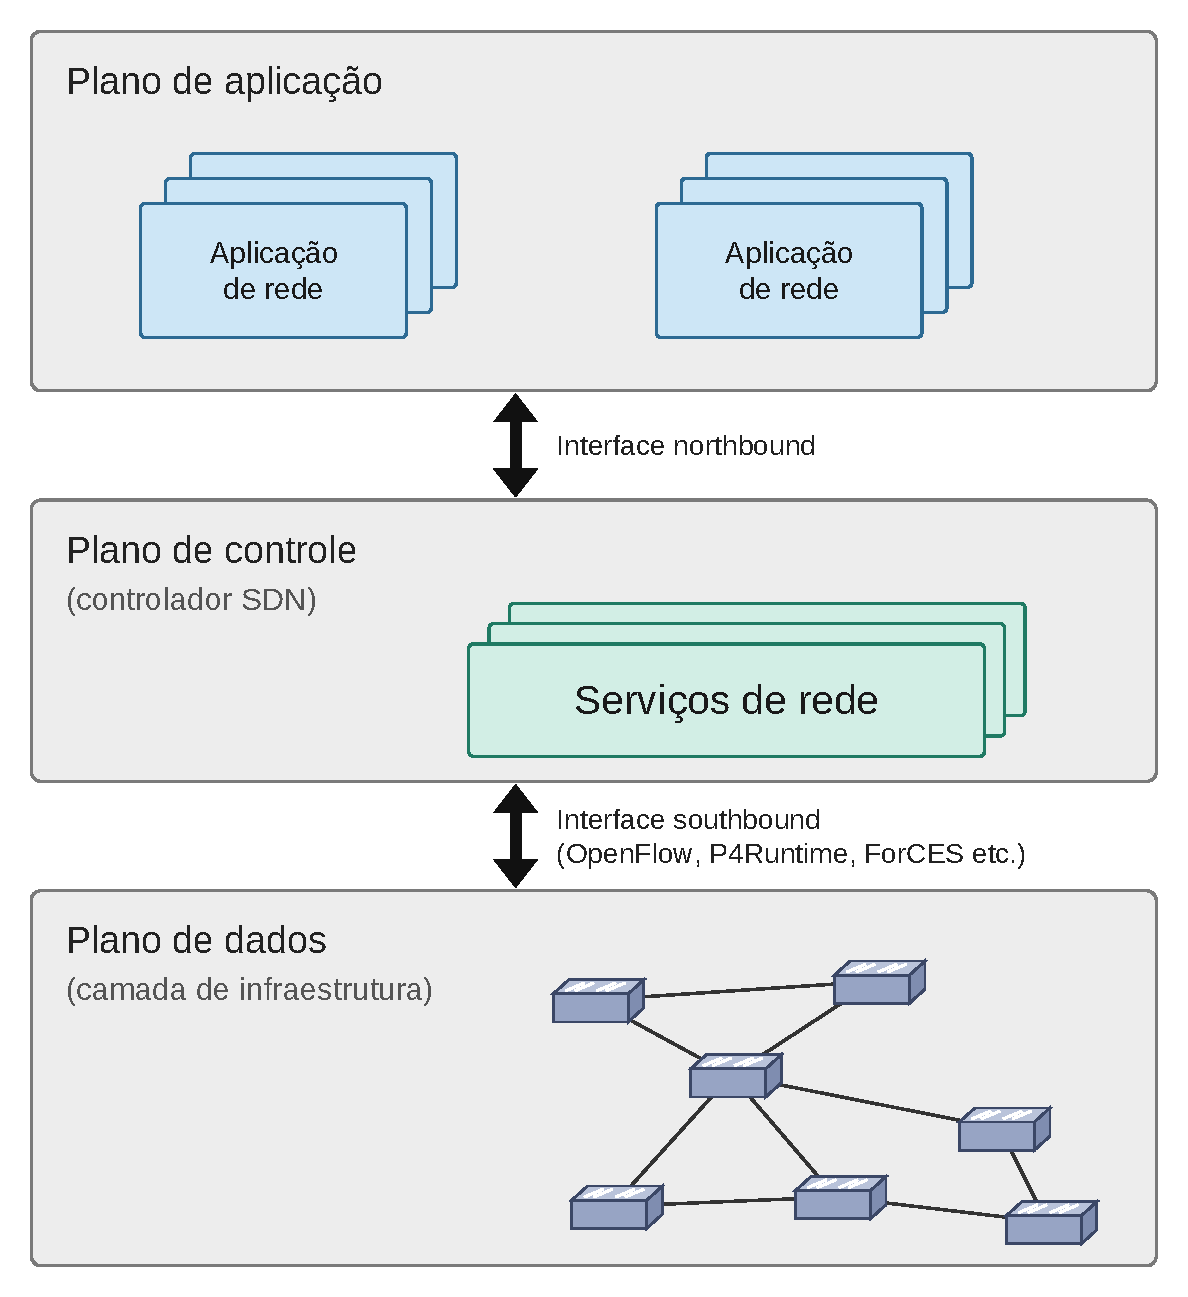
\includegraphics[width=0.6\textwidth]{figuras/arquitetura_sdn.pdf}
    \label{fig:arquitetura_sdn}
    \fonte{Adaptado de \textcite{katukam2013sdn}.}
\end{figure}

Ao centralizar logicamente o plano de controle em uma entidade denominada controlador SDN, a rede ganha visibilidade global e capacidade de abstração do hardware subjacente. Em contraposição aos modelos tradicionais, nos quais os dispositivos operam com inteligência distribuída e tabelas configuradas individualmente de forma autônoma ou estática, a abordagem SDN permite gerenciar políticas de segurança, balanceamento e alocação de largura de banda de maneira coordenada e automatizada a partir de um único núcleo de controle.

\subsection{Linguagem P4}
\label{subsec:linguagem_p4}

Os dispositivos de rede apresentam diferentes níveis de programabilidade consoante a sua arquitetura de concepção. Tradicionalmente, grande parte dos equipamentos em operação possui um plano de dados estático e fechado, o que restringe severamente a incorporação de novos protocolos e dificulta a avaliação empírica de propostas de encaminhamento não padronizadas pelos fabricantes.

A linguagem P4 (\textit{Programming Protocol-independent Packet Processors}) surge como uma linguagem de domínio específico concebida precisamente para especificar e programar a lógica de funcionamento do plano de dados em elementos de encaminhamento, como comutadores (\textit{switches}) e roteadores. Distinguindo-se da abordagem introduzida pelo OpenFlow --- que se apoiava em tabelas de fluxo com cabeçalhos e correspondências pré-definidas ---, o P4 outorga ao desenvolvedor a capacidade de determinar como os pacotes de rede devem ser descompactados (\textit{parsing}), analisados, modificados e reencaminhados de maneira totalmente independente de protocolos pré-estabelecidos. Torna-se, assim, viável a criação ou adaptação de formatos de cabeçalhos, a customização de primitivas de processamento e a especificação detalhada de cada etapa do \textit{pipeline} de comutação \cite{KAUR2021109}.

\begin{figure}[!htbp]
    \centering
    \caption{Fluxo de trabalho de um programa P4.}
    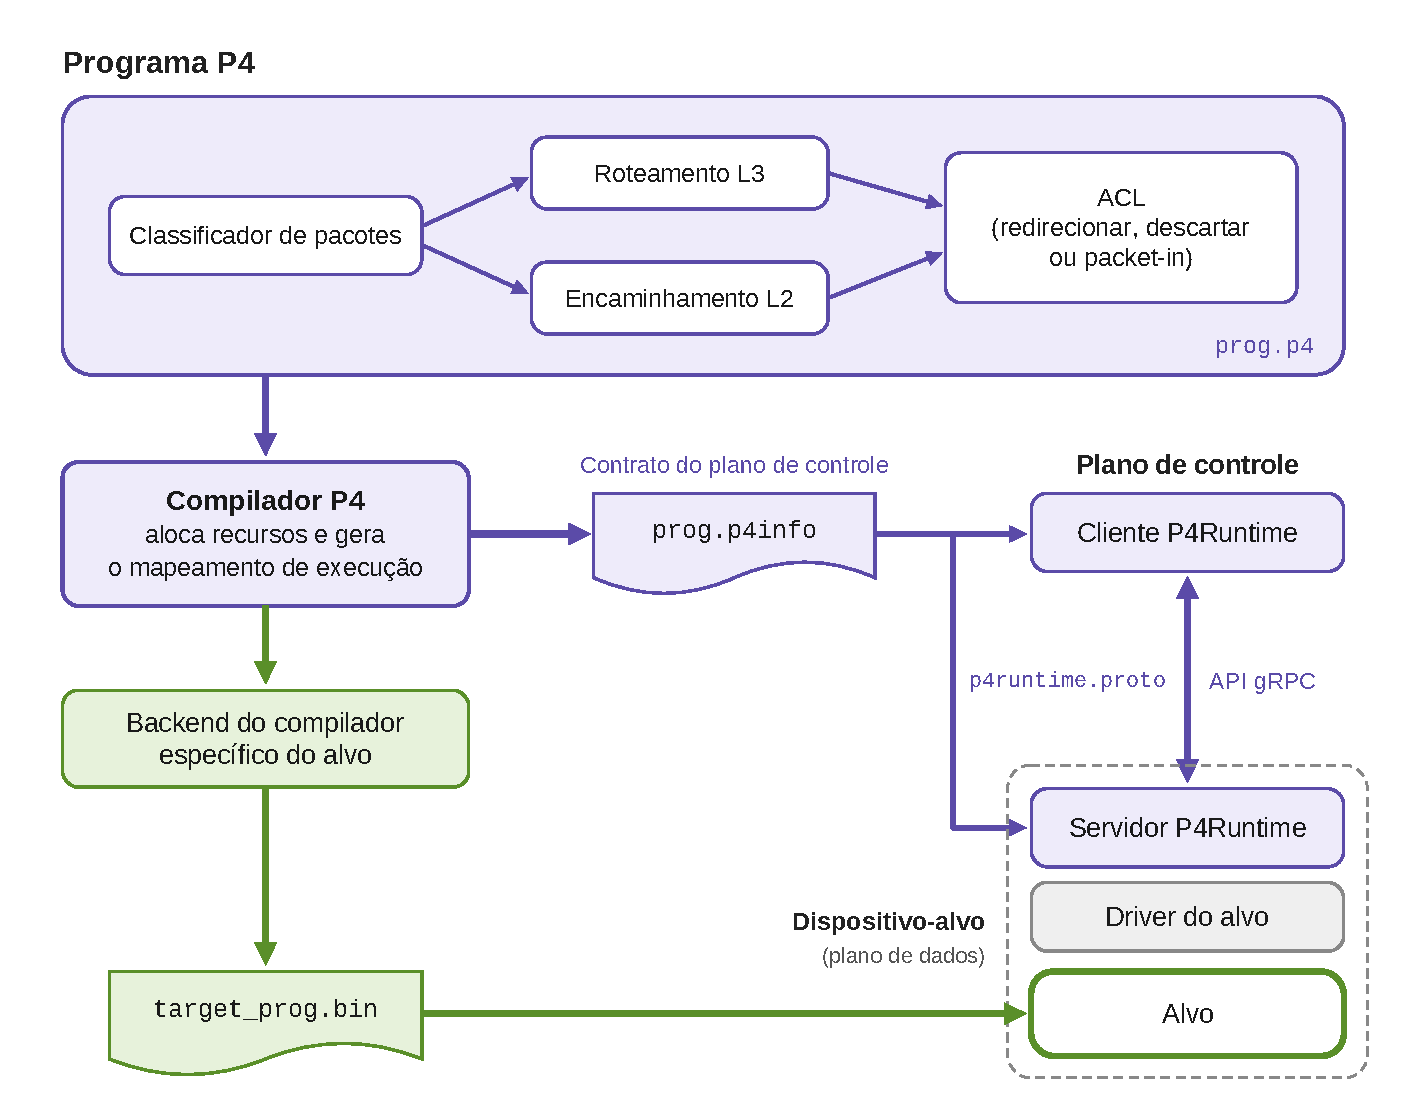
\includegraphics[width=0.85\textwidth]{figuras/fluxo_p4.pdf}
    \label{fig:fluxo-p4}
    \fonte{Adaptado de \textcite{p4org2025workflow}.}
\end{figure}

A Figura~\ref{fig:fluxo-p4} ilustra o fluxo de trabalho típico da programação de um dispositivo P4. Para cada alvo (\textit{target}), o fabricante fornece um modelo de arquitetura, que define os blocos programáveis e as interfaces disponíveis, e um compilador P4 específico. O compilador mapeia o programa P4 para os recursos desse alvo e gera dois artefatos: a configuração do plano de dados (\texttt{target\_prog.bin}), que implementa a lógica de processamento de pacotes descrita no programa, e o arquivo \texttt{P4Info} (\texttt{prog.p4info}), que atua como contrato entre os planos de controle e de dados, descrevendo as tabelas, ações e demais objetos gerenciados em tempo de execução por meio da API \textit{P4Runtime}.

Essa capacidade de parametrizar o processamento dos fluxos diretamente no circuito de encaminhamento constitui um marco na evolução das Redes Definidas por Software. Por intermédio do P4, projetistas e pesquisadores adquirem autonomia para conceber, homologar e implementar arquiteturas de encaminhamento e mecanismos de otimização de tráfego, prescindindo dos longos ciclos de atualização de \textit{firmware} fechado ou da substituição de plataformas proprietárias.

\subsection{Tecnologia eBPF e XDP}
\label{subsec:tecnologia_ebpf}

O \textit{Extended Berkeley Packet Filter} (eBPF) consiste em uma tecnologia de infraestrutura que atua como uma máquina virtual leve de 64~bits integrada ao núcleo (\textit{kernel}) do Linux, projetada para executar código customizado, seguro e de alto desempenho em tempo de execução sem requerer modificações no código-fonte nem a inclusão de módulos proprietários no sistema operacional \cite{sharaf2022extended}. Trata-se de uma evolução substancial da arquitetura clássica \textit{Berkeley Packet Filter} (cBPF) --- originalmente voltada apenas para a captura estática de pacotes e filtragem de chamadas de sistema ---, ampliando seu alcance para uma plataforma programável genérica e orientada a eventos, cujas instruções são compiladas dinamicamente em código de máquina nativo via JIT (\textit{Just-In-Time}) e submetidas a um rigoroso verificador estático (\textit{verifier}) in-kernel que assegura a terminação do programa e a segurança dos acessos à memória \cite{di2019berkeley}.

No âmbito do processamento de tráfego de rede e da implementação de Funções de Rede Virtualizadas (\textit{Network Functions Virtualization} -- NFV), o eBPF viabiliza a criação de planos de dados de alto rendimento ancorados diretamente aos pontos de acoplamento (\textit{hooks}) do subsistema de rede do Linux \cite{sharaf2022extended}, destacando-se dois níveis principais de atuação:
\begin{itemize}
    \item \textbf{\textit{eXpress Data Path} (XDP):} intercepta os pacotes diretamente no \textit{driver} da placa de rede (NIC) logo após a recepção pelo anel de entrada (\textit{Rx ring}) e antes da alocação da estrutura de metadados de rede do \textit{kernel} (\texttt{struct sk\_buff}), reduzindo drasticamente a sobrecarga de CPU para ações imediatas de descarte (\texttt{XDP\_DROP}), redirecionamento (\texttt{XDP\_REDIRECT}) ou reescrita de cabeçalhos \cite{miano2018creating};
    \item \textbf{\textit{Traffic Control} (TC BPF):} opera nos ganchos de ingresso e egresso do subsistema de controle de tráfego do Linux sobre a estrutura \texttt{struct \_\_sk\_buff}, permitindo tanto a inserção de novos cabeçalhos de encapsulamento quanto a integração direta com disciplinas nativas de enfileiramento e modelagem de tráfego (\textit{qdiscs}) \cite{sharaf2022extended}.
\end{itemize}

Por fim, a retenção de estado e o compartilhamento bidirecional de dados entre as rotinas em execução no núcleo e os processos de gestão no espaço do usuário (\textit{user space}) estruturam-se sobre os \textit{eBPF Maps} \cite{sharaf2022extended}. Essas estruturas do tipo chave-valor --- tais como tabelas \textit{hash}, arranjos e árvores de correspondência de prefixo mais longo (\textit{LPM Trie}) --- podem ser fixadas no sistema de arquivos virtual BPF (\texttt{/sys/fs/bpf}), permitindo a atualização dinâmica de políticas de encaminhamento e a coleta não intrusiva de telemetria \cite{miano2018creating}.

% ==============================================================================
\section{Protocolos de Roteamento na Origem}
\label{sec:roteamento_origem}

Os protocolos de Roteamento na Origem (\textit{Source Routing} -- SR) constituem um paradigma no qual a determinação da trajetória percorrida pelos pacotes é transferida dos elementos intermediários da infraestrutura para o nó emissor ou comutador de borda. Sob esse modelo, o ponto de ingresso define explicitamente a sequência de saltos necessária para alcançar o destino, encapsulando essas instruções diretamente em um cabeçalho específico anexado ao pacote \cite{dominicini2020}.

Essa abordagem concede à origem controle minucioso sobre o trajeto dos fluxos, sendo particularmente vantajosa para a imposição de políticas estritas de engenharia de tráfego, execução de testes de desempenho e monitoramento de enlaces. Embora a necessidade de conhecimento prévio da topologia completa represente um desafio em arquiteturas distribuídas convencionais, o \textit{Source Routing} integra-se de forma sinérgica com as Redes Definidas por Software (SDN), nas quais a visibilidade global do controlador central permite calcular percursos ótimos e codificar as decisões de encaminhamento diretamente nos pacotes na borda da rede \cite{ventre2020segment}.

No âmbito operacional, os protocolos de SR dividem-se em duas abordagens principais:
\begin{itemize}
    \item \textbf{Roteamento Estrito na Origem (\textit{Strict Source Routing}):} o trajeto é determinado de forma exata e mandatória, especificando cada nó intermediário e interface de saída no cabeçalho; o pacote deve transitar estritamente pela sequência delimitada, sem desvios;
    \item \textbf{Roteamento Livre na Origem (\textit{Loose Source Routing}):} a origem define apenas pontos-chave ou nós de passagem obrigatórios ao longo do percurso, enquanto os segmentos intermediários entre esses pontos são resolvidos dinamicamente por protocolos de roteamento convencionais.
\end{itemize}

Arquiteturas modernas como o \textit{Segment Routing} (SR-MPLS e SRv6) \cite{rfc8402, ventre2020segment} e o \textit{Path Switching} \cite{hari2015pathswitching} mitigam a manutenção de estados por fluxo no núcleo da rede. Contudo, as implementações baseadas em pilhas de segmentos (\textit{segment lists}) ainda exigem que os roteadores intermediários leiam, processem e removam ou atualizem ponteiros no cabeçalho a cada salto, além de gerarem sobrecarga de cabeçalho variável proporcional ao comprimento da rota \cite{dominicini2020}.

\subsection{O Protocolo PolKA}
\label{subsec:protocolo_polka}

Como alternativa aos modelos tradicionais de roteamento estrito na origem baseados em empilhamento de rótulos, a arquitetura \polka\ (\textit{Polynomial Key-based Architecture}) fundamenta seu mecanismo de encaminhamento no Sistema Numérico de Resíduos (\textit{Residue Number System} -- RNS) \cite{dominicini2020, Bajard2007}. A principal distinção do protocolo reside na capacidade de descrever trajetos arbitrários por meio de um modelo totalmente sem estado (\textit{stateless}) nos comutadores de núcleo, dispensando tanto consultas a tabelas de fluxo internas quanto a reescrita de cabeçalhos ao longo do trânsito dos pacotes. Isso é viabilizado pelo emprego da aritmética polinomial binária sobre o corpo finito de Galois de ordem 2, denominado $GF(2)$, cujas propriedades algébricas garantem a invariância do identificador de rota (\routeID) durante todo o percurso no domínio de transporte \cite{dominicini2020}.

A mecânica de comutação do \polka\ converte os roteadores de núcleo em elementos simplificados que executam exclusivamente operações de módulo polinomial. Formalmente, considere um pacote destinado a percorrer um caminho predefinido constituído por uma sequência ordenada de $N$ nós de núcleo e suas respectivas interfaces de saída. Cada nó participante $i$ ($i = 1, 2, \dots, N$) recebe um identificador unívoco denominado \nodeID, modelado por um polinômio irredutível $s_i(t) \in GF(2)[t]$, sendo todos os elementos do conjunto $S = \{s_1(t), s_2(t), \dots, s_N(t)\}$ coprimos entre si e com grau que satisfaz $\text{grau}(s_i(t)) \ge \lceil \log_2(\text{nports}) \rceil$, em que $\text{nports}$ representa o número de portas do dispositivo. Por sua vez, a interface de saída pretendida em cada salto é expressa por um polinômio de porta $o_i(t) \in GF(2)[t]$ com $\text{grau}(s_i(t)) > \text{grau}(o_i(t))$.

Com base na topologia e na sequência estipulada de saltos, o plano de controle sintetiza um único identificador de rota, o polinômio $R(t)$, por intermédio do Teorema Chinês dos Restos (CRT) polinomial \cite{Shoup:2009, dominicini2020}, de modo a satisfazer simultaneamente o seguinte sistema de congruências:

\begin{equation}
\label{eq:polka_crt}
R(t) \equiv o_i(t) \pmod{s_i(t)}, \quad \forall \, i \in \{1, 2, \dots, N\}
\end{equation}

Esse valor $R(t)$ calculado é inserido no cabeçalho do pacote unicamente no nó de ingresso (borda da rede). Ao receber o quadro, cada comutador de núcleo obtém sua interface local de encaminhamento de modo determinístico por meio da operação de resto da divisão polinomial entre o rótulo $R(t)$ e seu próprio identificador de nó, expressa por $o_i(t) = \langle R(t) \rangle_{s_i(t)} = R(t) \bmod s_i(t)$, a qual pode ser executada em taxa de linha (\textit{line-rate}) mediante o reuso de unidades de hardware de Verificação Cíclica de Redundância (CRC) \cite{dominicini2021}. Por conseguinte, elimina-se o tempo de convergência e a sobrecarga de sinalização no núcleo, visto que a criação ou migração de fluxos para novos caminhos exige unicamente a atualização das regras nos dispositivos de borda.

% ==============================================================================
\section{Redes Cientes de Caminho}
\label{sec:path_aware}

Na arquitetura tradicional da Internet, o encaminhamento de pacotes orienta-se pelo princípio fim a fim (\textit{end-to-end argument}), no qual a inteligência de controle de congestionamento e confiabilidade reside nos sistemas finais (\textit{endpoints}), enquanto os roteadores intermediários operam de maneira simplificada com base em tabelas locais e endereços de destino \cite{postel1981, borges2024pot}. Sob esse paradigma de melhor esforço (\textit{best-effort}), a infraestrutura de rede comporta-se como uma camada opaca: os pontos finais e os dispositivos de borda não dispõem de informações explícitas sobre as trajetórias disponíveis, tampouco conseguem selecionar ou auditar o caminho exato percorrido pelos fluxos \cite{trammell2022rfc, borges2024pot}. Como consequência, enlaces alternativos permanecem subutilizados, gargalos ocorrem em rotas padrão de menor contagem de saltos e torna-se inviável assegurar garantias granulares de Qualidade de Serviço (QoS) conforme os requisitos específicos de cada aplicação \cite{wei2026panqosr}.

Para superar essa assimetria entre a infraestrutura de transporte e as demandas das aplicações, emergem as Redes Cientes de Caminho (\textit{Path-Aware Networking} -- PAN) \cite{trammell2022rfc, borges2024pot}. Conforme sistematizado pelo grupo de pesquisa PANRG (\textit{Path Aware Networking Research Group}) do IRTF, uma arquitetura PAN expõe as propriedades topológicas e de desempenho dos caminhos disponíveis aos sistemas finais ou aos nós de borda da rede, capacitando-os a selecionar ou influenciar ativamente as rotas que seus pacotes deverão atravessar \cite{trammell2022rfc, wei2026panqosr}. Em contraposição ao modelo convencional passivo, a consciência de caminho fundamenta-se em três propriedades arquiteturais essenciais \cite{borges2024pot}:
\begin{itemize}
    \item \textbf{Visibilidade (\textit{Visibility}):} capacidade de descobrir, mensurar e disponibilizar informações precisas sobre as características estáticas e dinâmicas dos caminhos (tais como latência, largura de banda residual, \textit{jitter} e perda de pacotes), frequentemente apoiada por mecanismos de telemetria de rede \cite{trammell2022rfc, borges2024pot};
    \item \textbf{Controlabilidade (\textit{Controllability}):} capacidade de selecionar explicitamente a trajetória de encaminhamento por fluxo ou classe de serviço, permitindo que decisões de engenharia de tráfego adaptem-se dinamicamente às políticas da aplicação e às condições instantâneas da rede \cite{borges2024pot, wei2026panqosr};
    \item \textbf{Verificabilidade (\textit{Verifiability}):} capacidade de atestar que os pacotes transitaram efetivamente pela sequência de nós autorizada, mitigando desvios não intencionais ou maliciosos e assegurando a conformidade com os Acordos de Nível de Serviço (SLAs) \cite{borges2024pot}.
\end{itemize}

A Tabela~\ref{tab:comparacao_pan} sintetiza as principais diferenças estruturais entre o paradigma tradicional de roteamento na Internet e a abordagem de Redes Cientes de Caminho.

\begin{table}[!htb]
    \centering
    \caption{Comparação entre o roteamento tradicional na Internet e as Redes Cientes de Caminho (PAN).}
    \label{tab:comparacao_pan}
    \begin{tabular}{p{3.2cm} p{5.3cm} p{5.5cm}}
        \hline
        \textbf{Característica} & \textbf{Roteamento Tradicional} & \textbf{Redes Cientes de Caminho (PAN)} \\
        \hline
        \textbf{Seleção de Caminho} & Implícita, salto a salto (\textit{hop-by-hop}), baseada em métricas estáticas de destino. & Explícita, controlada na origem ou na borda com base nos requisitos do fluxo. \\
        \textbf{Visibilidade de Rota} & Infraestrutura opaca; diagnóstico indireto e limitado (e.g., \textit{traceroute}, SNMP). & Exposição de atributos de caminho e telemetria granular em tempo real. \\
        \textbf{Adaptação e QoS} & Estática ou de convergência lenta; tratamento homogêneo de melhor esforço. & Dinâmica e orientada a políticas por classe de tráfego ou aplicação. \\
        \textbf{Verificabilidade} & Ausente; sem garantias nativas sobre a trajetória percorrida no núcleo. & Suporte nativo à comprovação de trânsito e conformidade de políticas. \\
        \hline
    \end{tabular}
    \fonte{Elaborado pelo autor (2026), adaptado de \textcite{trammell2022rfc, borges2024pot}.}
\end{table}

Apesar dos benefícios evidentes, a adoção prática de arquiteturas PAN enfrenta desafios técnicos e operacionais relevantes, documentados na RFC~9217 \cite{trammell2022rfc}, entre os quais se destacam a escalabilidade na disseminação de métricas de caminho e o custo de manutenção de estado nos dispositivos intermediários \cite{trammell2022rfc, wei2026panqosr}. Iniciativas como a arquitetura SCION (\textit{Scalability, Control, and Isolation on Next-Generation Networks}) demonstram a viabilidade de redes PAN interdomínio ao agrupar sistemas autônomos em domínios de isolamento e delegar a seleção de caminhos aos pontos finais \cite{barrera2017scion}. Contudo, soluções baseadas em implantação limpa (\textit{clean-slate}) exigem alterações profundas nas pilhas de protocolos dos hospedeiros, dificultando a adoção incremental em redes de produção \cite{wei2026panqosr}.

Para viabilizar a implantação incremental sem modificar os sistemas finais, a literatura recente propõe deslocar a inteligência de consciência de caminho para os comutadores de borda (\textit{edge nodes}), combinando SDN, telemetria e protocolos de Roteamento na Origem \cite{dominicini2020, borges2024pot, wei2026panqosr}. Nesse contexto, o arcabouço PanQoSR \cite{wei2026panqosr} explora a disseminação de atributos de QoS para calcular rotas restritas a múltiplos objetivos e impô-las via \textit{Segment Routing}. De modo complementar, \textcite{puttaswamy2025pathaware} demonstram a transição de redes cientes de caminho para redes cientes de aplicação (\textit{Application-Aware Source Routing}), integrando classificação de tráfego na borda e escalonamento ponderado nas filas de saída para atender classes heterogêneas de serviço.

% ==============================================================================
\section{Fatiamento de Redes (\textit{Network Slicing})}
\label{sec:network_slicing}

O fatiamento de rede (\textit{network slicing}) é um paradigma arquitetural que permite particionar uma infraestrutura física compartilhada em múltiplas redes lógicas independentes, isoladas e personalizadas (\textit{slices}) \cite{afolabi2018network, FoukasXenofon2017NSi5}. Cada fatia combina recursos computacionais, de armazenamento e de transporte com funções de rede específicas (físicas ou virtualizadas), configuradas de ponta a ponta para satisfazer requisitos distintos de Qualidade de Serviço (QoS) e Acordos de Nível de Serviço (SLAs) \cite{itu.y3112, ZhangShunliang2019AOoN}. Em cenários multiserviço, essas demandas abrangem desde perfis de banda larga móvel aprimorada (\textit{enhanced Mobile Broadband} -- eMBB) e comunicações ultraconfiáveis de baixa latência (\textit{Ultra-Reliable Low Latency Communications} -- URLLC) até comunicações massivas tipo máquina (\textit{Massive IoT} / mMTC) \cite{3gpp.23.501, RostPeter2016Mnae}.

Em vez de depender de redes monolíticas incapazes de responder a requisitos antagônicos devido ao acoplamento rígido entre funções de rede e hardware dedicado, o fatiamento apoia-se em Redes Definidas por Software (SDN), Virtualização de Funções de Rede (NFV) e computação na borda para proporcionar controle programável e abstração de recursos \cite{BARAKABITZE2020106984, wijethilaka2021survey}. Historicamente, o conceito de partição de infraestruturas em fatias isoladas consolidou-se inicialmente em plataformas acadêmicas de experimentação distribuída (como PlanetLab e FlowVisor) e evoluiu para um pilar arquitetural formal nas especificações do 3GPP (Releases 15 a 18) \cite{3gpp.23.501, 3gpp.28.530} e da União Internacional de Telecomunicações (Recomendação ITU-T Y.3112) \cite{itu.y3112}.

\begin{figure}[!htbp]
    \centering
    \caption{Fatiamento lógico de uma infraestrutura física em múltiplas redes virtuais isoladas.}
    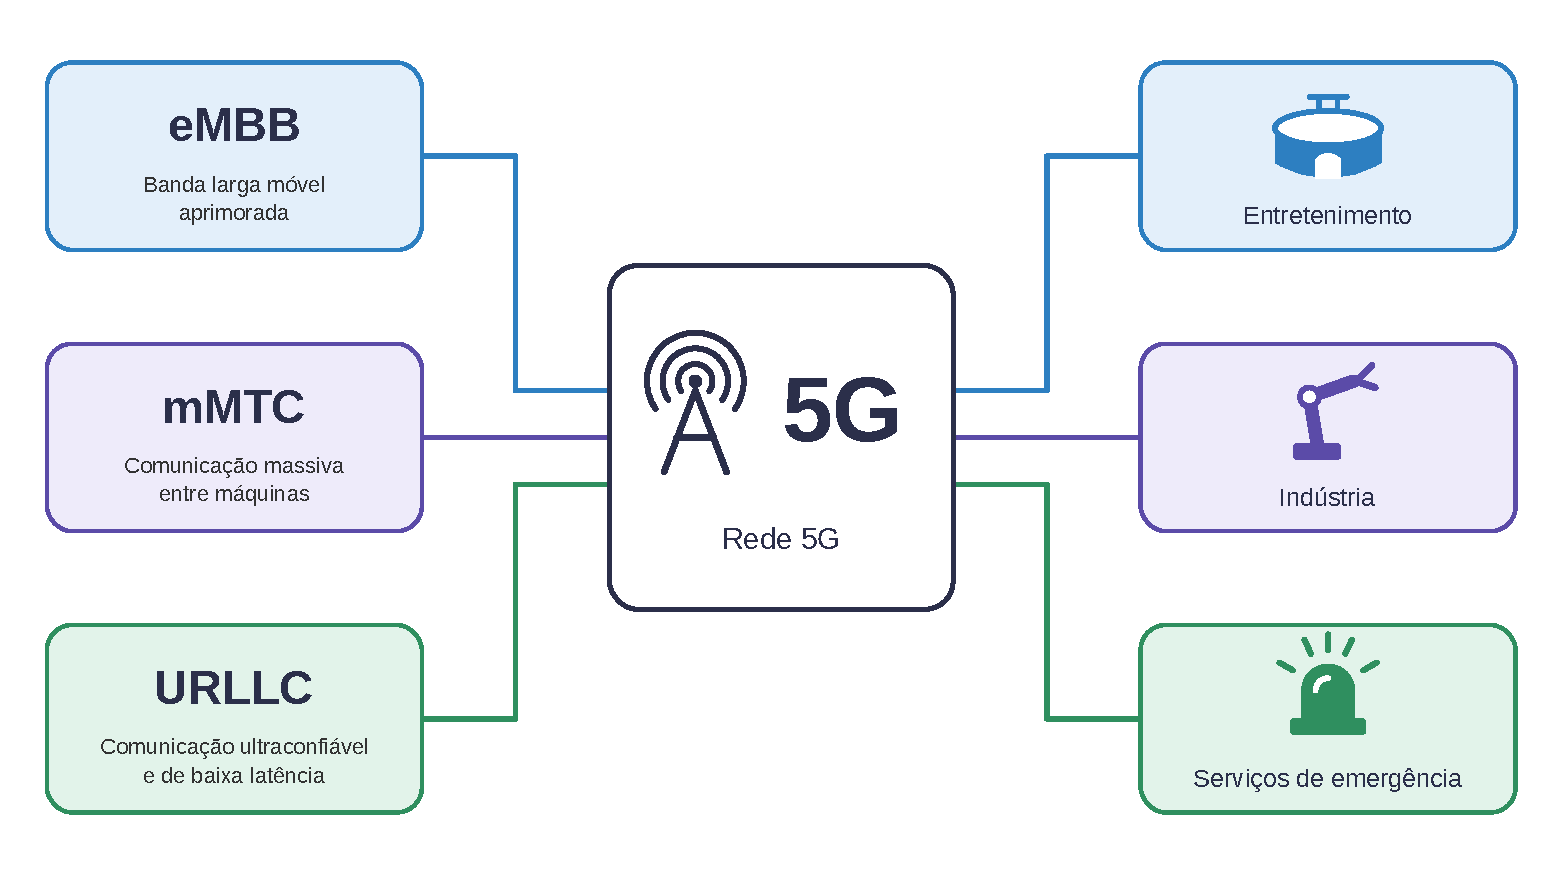
\includegraphics[width=0.6\textwidth]{figuras/fatiamento_5g.pdf}
    \label{fig:fatiamento_5g}
    \fonte{Adaptado de \textcite{inseego2026slicing}.}
\end{figure}

Conforme ilustrado na Figura~\ref{fig:fatiamento_5g}, um desafio crítico na concretização do fatiamento reside no mapeamento consistente entre os identificadores de fatia da camada de serviço (tais como o parâmetro S-NSSAI em redes 5G/6G ou marcações de classe de serviço na borda) e os mecanismos de isolamento na rede de transporte \cite{kotulski20205g, 8436847}. O isolamento entre fatias classifica-se fundamentalmente em dois níveis \cite{kotulski20205g}:
\begin{itemize}
    \item \textbf{Isolamento Lógico:} separação dos planos de controle, endereçamento e políticas de roteamento entre diferentes inquilinos (\textit{tenants}), impedindo vazamento de tráfego ou conflitos de configuração;
    \item \textbf{Isolamento de Desempenho:} garantia de que variações bruscas de carga, rajadas ou congestionamentos originados em uma fatia não degradem as métricas de vazão, latência ou perda de pacotes das demais fatias que compartilham os mesmos enlaces e roteadores físicos \cite{afolabi2018network, kotulski20205g}.
\end{itemize}

% ==============================================================================
\section{Qualidade de Serviço, Escalonamento e Controle de Congestionamento}
\label{sec:qos_escalonamento}

\subsection{Modelos de QoS e Diferenciação de Tráfego}
\label{subsec:modelos_qos}

Para prover isolamento de desempenho em redes de pacotes, duas arquiteturas clássicas foram padronizadas pelo IETF: os Serviços Integrados (\textit{Integrated Services} -- IntServ), baseados na reserva explícita de recursos por fluxo individual mediante sinalização (RSVP), cuja escalabilidade é severamente limitada pela necessidade de manter estados por fluxo em todos os roteadores do núcleo; e os Serviços Diferenciados (\textit{Differentiated Services} -- DiffServ), que agrupam o tráfego em classes agregadas na borda da rede por meio da marcação do campo DSCP (\textit{Differentiated Services Code Point}) no cabeçalho IP \cite{Laki2021, puttaswamy2025pathaware}.

Embora o modelo DiffServ escale adequadamente no núcleo ao eliminar estados por fluxo, sua eficácia depende diretamente das políticas de encaminhamento por salto (\textit{Per-Hop Behaviors} -- PHB) e dos algoritmos de escalonamento configurados nas interfaces de saída de cada comutador \cite{turkovic2021p4qos}. Sem o alinhamento entre a seleção da rota e o tratamento nas filas intermediárias, fluxos marcados com alta prioridade ainda podem sofrer degradação caso sejam encaminhados por enlaces congestionados ou mal dimensionados \cite{wei2026panqosr}.

\subsection{Disciplinas de Enfileiramento e Escalonamento Programável}
\label{subsec:disciplinas_filas}

Nos dispositivos de rede, quando a taxa de chegada de pacotes excede a capacidade instantânea de transmissão de uma interface de saída, os quadros são armazenados em \textit{buffers} e arbitrados por uma disciplina de escalonamento (\textit{packet scheduler}), cujo comportamento determina o atraso de enfileiramento, a variação do atraso (\textit{jitter}, definida pela RFC~3550) e a repartição da largura de banda entre os fluxos:

\begin{itemize}
    \item \textbf{FIFO (\textit{First-In, First-Out}):} disciplina padrão na qual todos os pacotes compartilham uma única fila e são servidos estritamente por ordem de chegada. Embora apresente complexidade computacional mínima, o FIFO não oferece qualquer isolamento: fluxos volumosos de longa duração (\textit{elephant flows}) preenchem o \textit{buffer} (\textit{bufferbloat}) e impõem atrasos elevados e imprevisíveis a fluxos curtos sensíveis à latência (\textit{mice flows}) \cite{santos2024mtspolka}.
    \item \textbf{Prioridade Estrita (\textit{Strict Priority} -- SP):} segrega o tráfego em múltiplas filas hierárquicas e garante que uma fila de menor precedência somente seja atendida quando todas as filas de prioridade superior estiverem completamente vazias. Embora minimize a latência e o \textit{jitter} de aplicações críticas, a prioridade estrita sem controle de admissão ou limitação de taxa pode provocar a inanição (\textit{starvation}) completa dos fluxos de menor prioridade \cite{Elbediwy2025}.
    \item \textbf{\textit{Weighted Deficit Round-Robin} (WDRR):} extensão ponderada do algoritmo \textit{Deficit Round-Robin} (DRR) que permite o compartilhamento justo e proporcional de largura de banda entre múltiplas filas com pacotes de tamanho variável, sem exigir conhecimento prévio do tamanho médio dos quadros \cite{4489385}. A cada ciclo, cada fila ativa recebe um crédito em bytes (\textit{quantum}) proporcional ao peso atribuído à sua classe de serviço; um pacote é transmitido se seu tamanho for inferior ou igual ao déficit acumulado da fila, preservando o saldo remanescente para a rodada seguinte. Além de evitar a inanição, o WDRR possui natureza conservadora de trabalho (\textit{work-conserving}), permitindo que filas ativas aproveitem dinamicamente a largura de banda ociosa de filas vazias \cite{4489385, Elbediwy2025}.
    \item \textbf{Escalonamento Híbrido (SP-WDRR):} combina filas de prioridade estrita no topo da hierarquia --- destinadas a tráfegos de tempo real ou sinalização crítica com taxa estritamente limitada --- com filas escalonadas via WDRR para o tráfego elástico restante, conciliando garantias determinísticas de baixa latência com repartição ponderada de banda.
\end{itemize}

Com o advento dos planos de dados programáveis, pesquisas recentes propuseram abstrações como o PIFO (\textit{Push-In First-Out}) \cite{Sivaraman2016}, o SP-PIFO \cite{Alcoz2020} e gerenciadores de tráfego programáveis baseados em classificações \cite{Elbediwy2024, Elbediwy2025} para superar a rigidez dos escalonadores fixos em comutadores P4 e emuladores como o BMv2. De forma complementar, no \textit{kernel} Linux, o subsistema \textit{Traffic Control} (\texttt{tc}) oferece implementações nativas de disciplinas hierárquicas e sem classes (como \texttt{drr}, \texttt{tbf}, \texttt{netem} e \texttt{bfifo}), permitindo que programas eBPF direcionem pacotes diretamente às filas de saída por meio de metadados do \texttt{sk\_buff} \cite{sharaf2022extended}.

\subsection{Algoritmos de Controle de Congestionamento: CUBIC e BBR}
\label{subsec:controle_congestionamento}

O desempenho observado pelas aplicações em redes fatiadas também sofre influência direta dos algoritmos de controle de congestionamento executados na camada de transporte dos hospedeiros, os quais determinam como os fluxos TCP disputam a capacidade residual das filas:

\begin{itemize}
    \item \textbf{CUBIC (Baseado em Perda):} algoritmo padrão na maioria das distribuições Linux modernas, que ajusta a janela de congestionamento (\textit{cwnd}) segundo uma função cúbica do tempo decorrido desde o último evento de perda de pacotes. Por depender do descarte de pacotes para detectar o congestionamento, o CUBIC tende a preencher continuamente os \textit{buffers} dos roteadores intermediários até provocar perdas, gerando um comportamento oscilatório em dente de serra e elevando o atraso de enfileiramento \cite{Laki2021}.
    \item \textbf{BBR (\textit{Bottleneck Bandwidth and Round-trip propagation time} -- Baseado em Modelo):} em vez de utilizar a perda de pacotes como sinal primário de congestionamento, o BBR estima continuamente duas grandezas fundamentais do caminho: a largura de banda máxima disponível no gargalo (\textit{BtlBw}) e o menor tempo de ida e volta de propagação (\textit{RTprop}). A partir dessas estimativas, o algoritmo regula a cadência de envio (\textit{pacing}) para manter o volume de dados em trânsito próximo ao produto banda-atraso (\textit{Bandwidth-Delay Product} -- BDP), alternando fases periódicas de sondagem de banda e de latência mínima (\textit{ProbeRTT}) a fim de maximizar a vazão sem saturar as filas da rede.
\end{itemize}

% ==============================================================================
\section{Trabalhos Relacionados}
\label{sec:trabalhos_relacionados}

Diversas propostas na literatura investigam a provisão de Qualidade de Serviço, engenharia de tráfego e fatiamento em planos de dados programáveis e redes cientes de caminho. A Tabela~\ref{tab:trabalhos_relacionados} apresenta uma síntese comparativa entre as principais abordagens correlatas e a arquitetura \nome\ proposta nesta dissertação.

\begin{table}[!htb]
    \centering
    \caption{Comparação entre trabalhos relacionados e a arquitetura \nome.}
    \label{tab:trabalhos_relacionados}
    \begin{tabularx}{\textwidth}{Xcccc}
        \toprule
        \textbf{Proposta / Referência} & \textbf{\shortstack{Núcleo sem\\Estado}} & \textbf{\shortstack{Rota Explícita\\na Origem}} & \textbf{\shortstack{Seleção de Fila\\por Salto}} & \textbf{\shortstack{Escalonamento\\Ponderado}} \\
        \midrule
        \textbf{Segment Routing} \cite{rfc8402}        & Parcial\textsuperscript{*} & Sim & Não & Não \\
        \textbf{RDNA} \cite{liberato2018rdna}          & Sim & Sim & Não & Não \\
        \textbf{ProgLab} \cite{froes2020proglab}       & Sim & Sim & Sim & Não \\
        \textbf{PolKA} \cite{dominicini2020}           & Sim & Sim & Não & Não \\
        \textbf{P4QoS / Virtual Queues} \cite{turkovic2021p4qos, harkous2021virtual} & Não & Não & Sim & Sim \\
        \textbf{SP-PIFO / TM Prog.} \cite{Alcoz2020, Elbediwy2025} & Não & Não & Sim & Sim \\
        \textbf{PanQoSR} \cite{wei2026panqosr}         & Parcial\textsuperscript{*} & Sim & Não & Não \\
        \textbf{App-Aware SR} \cite{puttaswamy2025pathaware} & Parcial\textsuperscript{*} & Sim & Indireta\textsuperscript{**} & Sim \\
        \midrule
        \textbf{SPolKA (Este Trabalho)}                & \textbf{Sim} & \textbf{Sim} & \textbf{Sim} & \textbf{Sim} \\
        \bottomrule
    \end{tabularx}
    \fonte{Elaborado pelo autor (2026). \textsuperscript{*}Exige remoção ou atualização de rótulos a cada salto. \textsuperscript{**}Baseada em mapeamento DiffServ/DSCP tradicional.}
\end{table}

As soluções baseadas em escalonamento programável no plano de dados, tais como P4QoS \cite{turkovic2021p4qos}, filas virtuais em P4 \cite{harkous2021virtual}, gerenciamento ativo de filas (\textit{Active Queue Management} -- AQM) em P4 \cite{kundel2018p4, papagianni2019pi2, qiao2022fine}, filas multinível \cite{iqbal2023p4}, SP-PIFO \cite{Alcoz2020} e gerenciadores de tráfego programáveis baseados em classificação \cite{Elbediwy2025}, oferecem controle refinado sobre o atraso e a repartição de banda nas interfaces de saída. Entretanto, essas abordagens concentram-se exclusivamente no comportamento local de enfileiramento dos comutadores, dependendo de tabelas de fluxo e manutenção de estado por classe ou fluxo no núcleo, sem integração nativa com roteamento explícito na origem.

No domínio do roteamento na origem e redes cientes de caminho, propostas como o \textit{Segment Routing} \cite{rfc8402}, o PanQoSR \cite{wei2026panqosr} e o roteamento ciente de aplicação de \textcite{puttaswamy2025pathaware} permitem direcionar fluxos por trajetórias com restrições de QoS. Contudo, o empilhamento de identificadores de segmento exige manipulação de cabeçalhos a cada salto, enquanto o tratamento de filas permanece desacoplado do rótulo de roteamento, dependendo de marcações estáticas como DSCP ou MPLS TC. De modo análogo, o encaminhamento sem estado no núcleo baseado em núcleo sem estado com QoS de \textcite{Laki2021} desacopla atraso e largura de banda, mas não oferece controle explícito de trajetória na origem.

Por fim, entre as arquiteturas baseadas no Sistema Numérico de Resíduos (RNS), a RDNA \cite{liberato2018rdna} e o ProgLab \cite{froes2020proglab} demonstraram a viabilidade de codificar caminhos e rótulos de QoS em identificadores residuais. Entretanto, ambos empregam aritmética modular inteira de precisão arbitrária, cujas operações de divisão inteira não são suportadas nativamente em taxa de linha pelos comutadores programáveis comerciais. Por outro lado, o protocolo \polka\ \cite{dominicini2020} e suas extensões para telemetria \cite{pereira2024mpolkaint}, comprovação de trânsito \cite{borges2024pot} e divisão multicaminho \cite{santos2024mtspolka} superaram a barreira computacional ao migrar para a aritmética polinomial em $GF(2)$ via unidades de CRC, mas restringiram-se à seleção de interfaces físicas de saída sem suporte a filas de serviço.

O protocolo \nome\ preenche exatamente essa lacuna ao estender a aritmética polinomial em $GF(2)$ do \polka\ para codificar, em um único rótulo imutável inserido na borda, tanto a porta de saída quanto a fila de serviço em cada salto, acoplando a decodificação sem estado no núcleo a escalonadores ponderados (WDRR e SP-WDRR) tanto em ambientes P4 quanto no \textit{kernel} Linux via eBPF/XDP.

% ---
% ------------------------  PROPOSTA ------------------------
% ---

\chapter{PROPOSTA}
\label{chap:proposta}

Este capítulo apresenta o projeto detalhado, os requisitos e a arquitetura da solução \nome\ (\textit{Slice-aware Polynomial Key-based Architecture}), concebida para abordar as limitações de escalabilidade, inflexibilidade do plano de dados e isolamento de Qualidade de Serviço (QoS) no fatiamento de redes cientes de caminho descritas no Capítulo~\ref{chap:introducao}.

A proposta unifica o roteamento na origem sem estados no núcleo --- baseado em Sistemas de Numeração de Resíduos (\textit{Residue Number System} -- RNS) e aritmética polinomial sobre o corpo finito de Galois $GF(2)$ --- com mecanismos programáveis de enfileiramento e escalonamento de pacotes. Ao delegar a classificação e a codificação das políticas de rede exclusivamente aos nós de borda, o \nome\ permite que os comutadores de núcleo executem o encaminhamento e a seleção de filas de prioridade em taxa de linha (\textit{line-rate}) sem a necessidade de manutenção de tabelas de estado por fluxo ou por fatia.

% ==============================================================================
\section{Levantamento de Requisitos}
\label{sec:requisitos}

Para suportar o fatiamento de redes (\textit{Network Slicing}) em redes cientes de caminho --- nas quais coexistem fluxos e aplicações heterogêneas com requisitos antagônicos de vazão, atraso e confiabilidade ---, a arquitetura de transporte deve garantir isolamento lógico e de desempenho sem comprometer a escalabilidade do plano de controle. Com base na análise da literatura e nas lacunas identificadas nos trabalhos relacionados, foram estabelecidos os requisitos funcionais (RF) e não funcionais (RNF) que norteiam o projeto do \nome, sintetizados nas Tabelas~\ref{tab:req_funcionais} e~\ref{tab:req_nao_funcionais}.

\begin{table}[htb]
    \centering
    \caption{Requisitos Funcionais da arquitetura \nome.}
    \label{tab:req_funcionais}
    \begin{tabular}{p{1.8cm} p{12.5cm}}
        \hline
        \textbf{Código} & \textbf{Descrição do Requisito Funcional} \\
        \hline
        \textbf{RF01} & \textbf{Codificação unificada de rota e QoS:} Codificar, em um único rótulo de comprimento fixo inserido na borda da rede, tanto a trajetória explícita quanto a política de enfileiramento para cada salto do caminho. \\
        \textbf{RF02} & \textbf{Encaminhamento e seleção de fila sem estados no núcleo:} Permitir que os comutadores de núcleo determinem simultaneamente a interface de egresso e o identificador da fila de serviço por meio de operações aritméticas locais, eliminando tabelas de roteamento e de QoS por fatia no núcleo. \\
        \textbf{RF03} & \textbf{Classificação flexível e mapeamento de fatias na borda:} Classificar os fluxos ingressantes a partir de qualquer campo de cabeçalho ou metadado de serviço (tais como marcações DSCP, etiquetas VLAN/PCP, rótulos MPLS TC, prefixos IP, portas L4 ou identificadores de fatia) e encapsulá-los com o respectivo rótulo de rota e QoS. \\
        \textbf{RF04} & \textbf{Isolamento de recursos via escalonamento ponderado:} Viabilizar garantias mínimas de largura de banda e priorização entre fatias concorrentes ao direcionar os pacotes para filas previamente configuradas sob políticas de escalonamento ponderado nas interfaces de saída, evitando a inanição (\textit{starvation}) de filas de menor prioridade. \\
        \textbf{RF05} & \textbf{Reconfiguração ágil de rotas e políticas:} Viabilizar a migração dinâmica de caminhos e a alteração de classes de serviço de uma fatia em tempo de execução mediante a atualização exclusiva das regras nos nós de borda. \\
        \hline
    \end{tabular}
    \fonte{Elaborado pelo autor (2026).}
\end{table}

\begin{table}[htb]
    \centering
    \caption{Requisitos Não Funcionais da arquitetura \nome.}
    \label{tab:req_nao_funcionais}
    \begin{tabular}{p{1.8cm} p{12.5cm}}
        \hline
        \textbf{Código} & \textbf{Descrição do Requisito Não Funcional} \\
        \hline
        \textbf{RNF01} & \textbf{Processamento em taxa de linha (\textit{line-rate}):} As operações de decodificação de rota e fila no plano de dados devem explorar primitivas nativas de hardware ou do núcleo do sistema operacional (como unidades de CRC e ganchos eBPF/XDP), garantindo latência determinística e alto desempenho. \\
        \textbf{RNF02} & \textbf{Baixa sobrecarga no plano de controle:} Eliminar a necessidade de sinalização e atualização coordenada em múltiplos dispositivos intermediários durante a criação, modificação ou remoção de fatias de rede. \\
        \textbf{RNF03} & \textbf{Imutabilidade e compacidade de cabeçalho:} Manter o cabeçalho de transporte com tamanho fixo e inalterado ao longo de todo o domínio de núcleo, evitando operações de reescrita ou remoção de rótulos salto a salto. \\
        \textbf{RNF04} & \textbf{Portabilidade arquitetural:} Permitir a implantação do plano de dados tanto em ambientes de emulação programável (e.g., P4/BMv2) quanto em planos de dados de alto desempenho baseados em hardware programável (e.g., Intel Tofino) ou no \textit{kernel} Linux (eBPF/XDP). \\
        \hline
    \end{tabular}
    \fonte{Elaborado pelo autor (2026).}
\end{table}

% ==============================================================================
\section{Arquitetura do Protocolo SPolKA}
\label{sec:arquitetura_spolka}

O protocolo \nome\ estende a arquitetura de roteamento na origem PolKA (\textit{Polynomial Key-based Architecture}) \cite{dominicini2020} ao incorporar, de forma nativa e sem estados no núcleo, o endereçamento de filas de serviço para o fatiamento em redes cientes de caminho. Enquanto abordagens tradicionais de roteamento na origem baseadas em empilhamento de rótulos exigem que cada salto remova ou atualize o cabeçalho --- incorrendo em sobrecarga crescente proporcional ao diâmetro da rede ---, o \nome\ codifica toda a trajetória e as respectivas políticas de QoS em um único identificador compacto e imutável ao longo do núcleo.

Estruturalmente, a arquitetura do \nome\ organiza-se em três camadas funcionais desacopladas, conforme ilustrado na Figura~\ref{fig:spolka_camadas}, seguindo o paradigma de Redes Definidas por Software (SDN) com planos de dados programáveis:
\begin{itemize}
    \item \textbf{Camada de Serviço:} Compreende as aplicações finais, funções de rede virtuais e sistemas de orquestração de fatias em redes cientes de caminho que demandam garantias específicas de Acordo de Nível de Serviço (SLA), expressas por meio de classes de tráfego diferenciadas ou identificadores de fatia.
    \item \textbf{Camada de Controle e Orquestração:} Centraliza a inteligência da rede e subdivide-se em quatro módulos lógicos: (i) \textit{Conhecimento da topologia}, responsável por mapear a infraestrutura física e monitorar o estado dos enlaces; (ii) \textit{Cálculo de caminhos}, que seleciona a sequência de saltos adequada aos requisitos de QoS de cada fatia; (iii) \textit{Geração polinomial do \routeID\ (CRT)}, encarregado de atribuir identificadores únicos aos nós e sintetizar os rótulos de rota e fila via Teorema Chinês dos Restos; e (iv) \textit{Políticas de filas (\qID\ e pesos WDRR)}, que define as configurações dos escalonadores e instala proativamente as regras de classificação nas tabelas dos comutadores de borda.
    \item \textbf{Camada de Infraestrutura Física (Plano de Dados):} Constituída por elementos de encaminhamento programáveis (como dispositivos habilitados para P4 ou \textit{hosts}/roteadores executando eBPF/XDP) divididos logicamente entre nós de borda --- que executam a classificação, o encapsulamento e o desencapsulamento dos rótulos --- e nós de núcleo, que operam de forma totalmente \textit{stateless} no encaminhamento e na seleção das filas dos pacotes.
\end{itemize}

\begin{figure}[!htb]
    \centering
    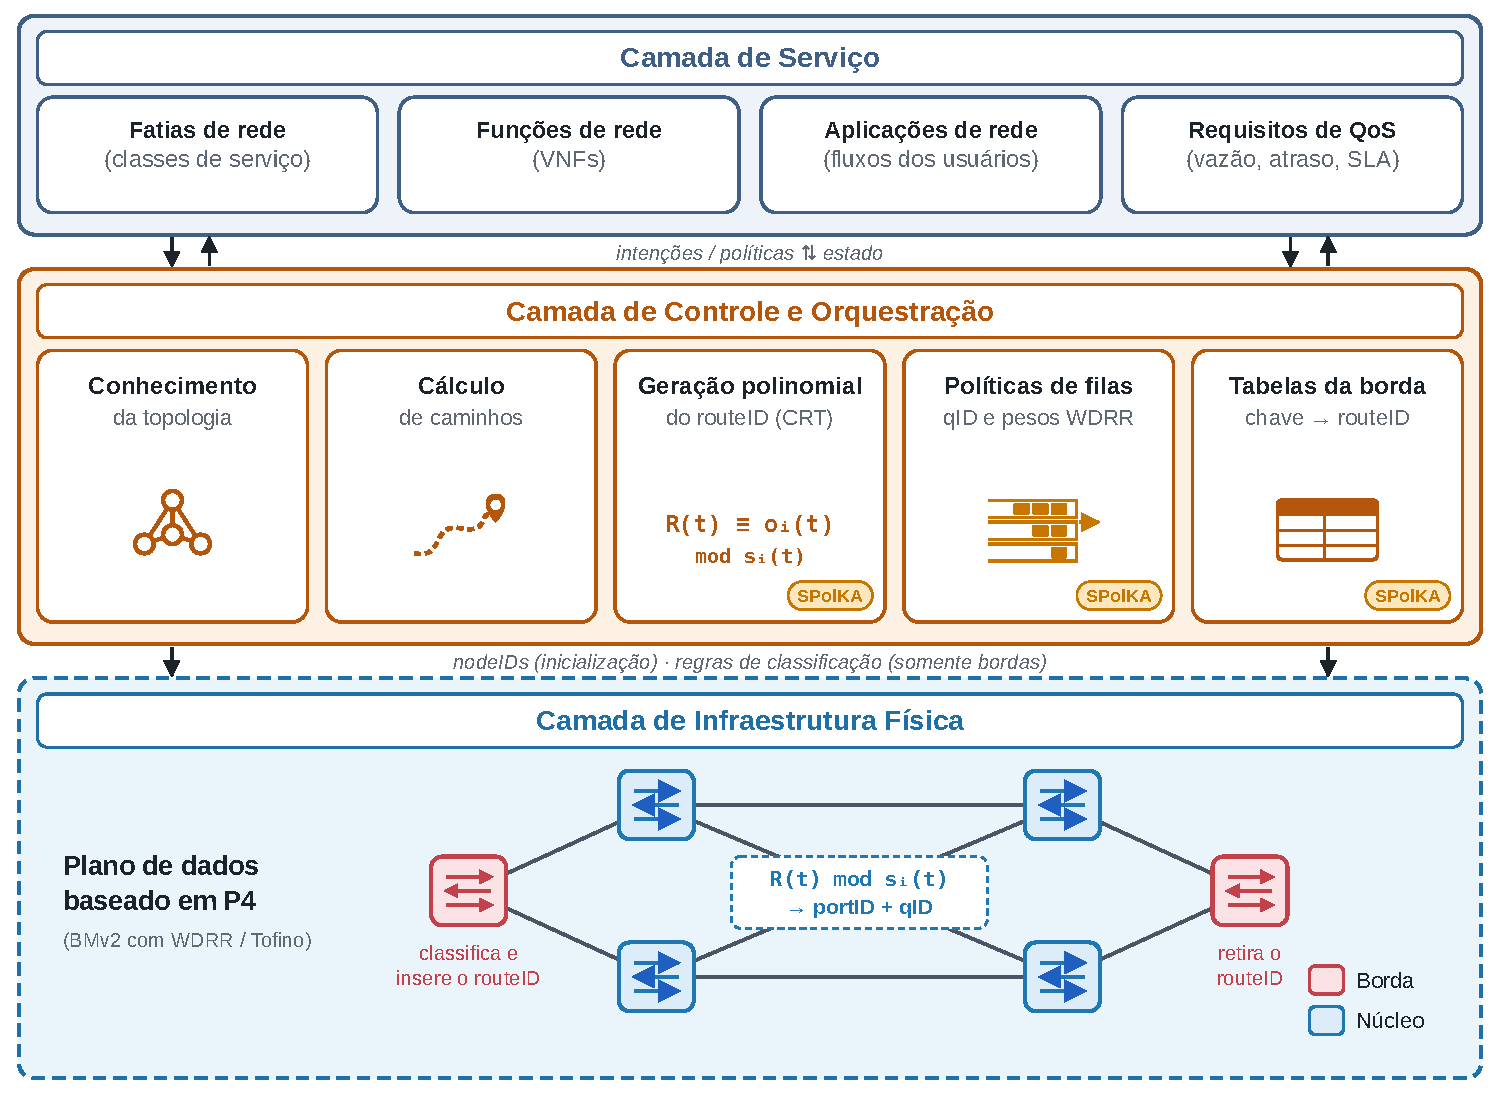
\includegraphics[width=\textwidth]{figuras/fig_arq_camadas_spolka.pdf}
    \captionsetup{justification=centering}
    \caption{Arquitetura em camadas do \nome\ e interação entre serviço, controle e plano de dados.}
    \label{fig:spolka_camadas}
\end{figure}

\subsection{Formulação Matemática e Codificação em $GF(2)$}
\label{subsec:formulacao_matematica}

O funcionamento operacional da arquitetura divide-se logicamente em três etapas principais: (i) a atribuição de identificadores e o cálculo do rótulo no Plano de Controle; (ii) a classificação e o encapsulamento na borda de ingresso; e (iii) o encaminhamento e a seleção de fila sem estados nos comutadores de núcleo.

Para formalizar o processo de codificação, considere um fluxo de tráfego de uma fatia que deve atravessar um caminho selecionado composto por $N$ nós de núcleo. Na fase de inicialização da topologia, o Controlador atribui a cada comutador de núcleo um identificador único representado por um polinômio irredutível $s_i(t)$ sobre o corpo finito de Galois $GF(2)$, formando o conjunto ordenado $S = \{s_1(t), s_2(t), \ldots, s_N(t)\}$ dos \nodeIDs\ ao longo do trajeto. Para garantir a unicidade da solução matemática, os polinômios pertencentes ao conjunto $S$ devem ser necessariamente coprimos entre si.

Simultaneamente, o Controlador define as ações de encaminhamento e priorização que cada nó intermediário deverá executar. Para cada salto $i \in \{1, 2, \ldots, N\}$, estabelece-se um polinômio de saída $o_i(t)$, pertencente ao conjunto $O = \{o_1(t), o_2(t), \ldots, o_N(t)\}$. Diferentemente da abordagem original do PolKA, na qual o resíduo codifica exclusivamente a interface de egresso, no \nome\ o polinômio $o_i(t)$ resulta da concatenação binária entre o identificador da porta física de saída (\portID) e o identificador da fila de serviço (\qID) atribuída ao fluxo naquele nó. Para que a recuperação dessa informação ocorra sem ambiguidades na operação de módulo, cada par de polinômios deve satisfazer estritamente a restrição de grau dada por $\text{grau}(s_i) > \text{grau}(o_i)$.

De posse dos conjuntos $S$ e $O$, o Controlador sintetiza o identificador global da fatia e da rota, denominado \routeID\ e representado pelo polinômio $R(t)$, por meio da aplicação do Teorema Chinês dos Restos (CRT) polinomial \cite{Shoup:2009, dominicini2020}. O polinômio $R(t)$ é calculado de modo a satisfazer simultaneamente o seguinte sistema de congruências lineares em $GF(2)$:

\begin{equation}
\label{eq:crt_spolka}
R(t) \equiv o_i(t) \pmod{s_i(t)}, \quad \forall i \in \{1, 2, \ldots, N\}
\end{equation}

Uma vez computado o \routeID, o Controlador traduz a política de engenharia de tráfego instalando regras de correspondência (\textit{match-action}) exclusivamente nos comutadores de borda da rede. No nó de ingresso, o tráfego entrante pode ser classificado a partir de qualquer campo de cabeçalho ou metadado de serviço --- tais como marcações DiffServ (DSCP), etiquetas VLAN/PCP, rótulos MPLS TC, prefixos IP, portas da camada de transporte ou identificadores de fatia --- e associado ao respectivo \routeID, que é então inserido no cabeçalho do pacote. Graças às propriedades aritméticas dos polinômios sobre $GF(2)$, o rótulo $R(t)$ permanece inalterado durante todo o percurso pelo domínio de transporte, sendo removido apenas pelo comutador de egresso antes da entrega ao destino final.

No plano de dados dos comutadores de núcleo, o encaminhamento opera de maneira totalmente desprovida de estados de fluxo (\textit{stateless}), eliminando a necessidade de tabelas de roteamento ou de manutenção de contexto por fatia. Ao receber um pacote encapsulado, cada nó de núcleo $i$ extrai simultaneamente a porta de destino e a fila de escalonamento calculando o resto da divisão polinomial (operação de módulo) entre o \routeID\ contido no cabeçalho e o seu próprio \nodeID\ localmente armazenado:

\begin{equation}
\label{eq:mod_spolka}
o_i(t) = \langle R(t) \rangle_{s_i(t)} = R(t) \bmod s_i(t)
\end{equation}

Em termos de implementação em hardware programável ou planos de dados acelerados (como P4 e eBPF), essa operação aritmética em $GF(2)$ equivale diretamente ao cálculo de verificação cíclica de redundância (CRC), permitindo sua execução em taxa de linha (\textit{line-rate}) com latência determinística. O valor binário resultante $o_i(t)$ é então particionado por meio de operações simples de deslocamento e mascaramento de bits (\textit{bit-slicing}): os bits mais significativos determinam o \portID\ para o qual o pacote deve ser comutado, enquanto os bits menos significativos especificam o \qID\ no gerenciador de tráfego (\textit{Traffic Manager}) da interface de saída. Ao direcionar os fluxos para filas previamente configuradas sob políticas de escalonamento ponderado nos nós intermediários, o \nome\ viabiliza o isolamento de largura de banda entre fatias concorrentes sem manter estado no núcleo.

\begin{figure}[!htb]
    \centering
    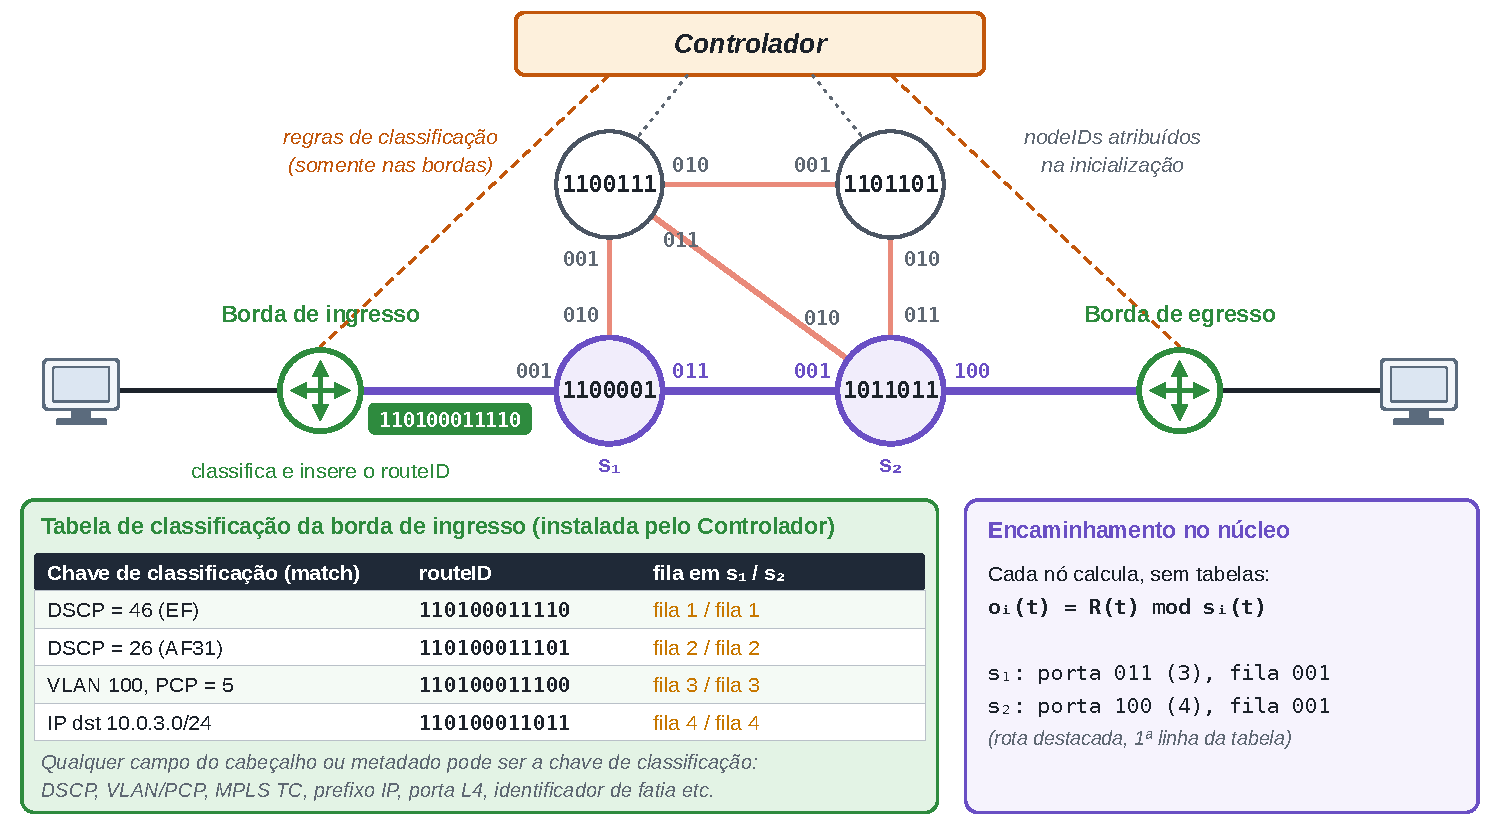
\includegraphics[width=\textwidth]{figuras/fig_arq1_visao_geral.pdf}
    \captionsetup{justification=centering}
    \caption{Visão geral da arquitetura \nome\ e tabela de classificação flexível na borda de ingresso.}
    \label{fig:spolka_visao_geral}
\end{figure}

A Figura~\ref{fig:spolka_visao_geral} apresenta a visão geral da arquitetura \nome\ e a operação do plano de dados na borda em uma topologia ciente de caminho cujos identificadores atribuídos pelo Controlador incluem os polinômios $s_1(t) = t^6 + t^5 + 1$ (representado em binário por $1100001$) e $s_2(t) = t^6 + t^4 + t^3 + t + 1$ ($1011011$). Para estabelecer o caminho $s_1 \rightarrow s_2$ com políticas específicas de enfileiramento em cada salto, o Controlador aplica o CRT polinomial (Equação~\ref{eq:crt_spolka}) e obtém o rótulo $R(t) = 110100011110$, associando-o à respectiva chave de classificação (como $\text{DSCP} = 46$, VLAN ou prefixo IP) na tabela de fluxo da borda de ingresso.

\begin{figure}[!htb]
    \centering
    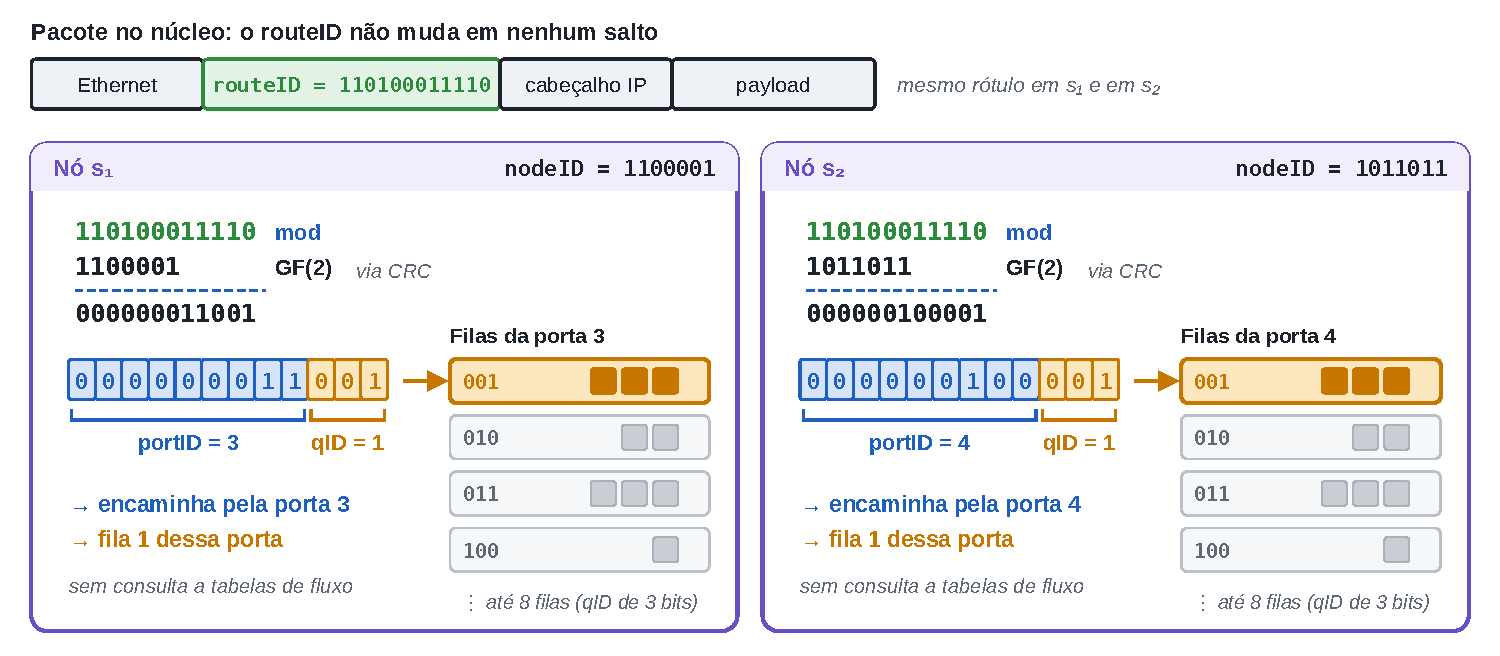
\includegraphics[width=\textwidth]{figuras/fig_arq2_nucleo.pdf}
    \captionsetup{justification=centering}
    \caption{Processamento sem estado (\textit{stateless}) e extração simultânea de porta e fila nos comutadores de núcleo do \nome.}
    \label{fig:spolka_nucleo}
\end{figure}

O detalhamento da operação executada internamente nos nós intermediários é ilustrado na Figura~\ref{fig:spolka_nucleo}. Quando o pacote alcança o primeiro nó de núcleo ($s_1$), o comutador executa a divisão polinomial em $GF(2)$ (via CRC) entre o rótulo imutável $R(t) = 110100011110$ e seu identificador local $s_1(t) = 1100001$ (Equação~\ref{eq:mod_spolka}), extraindo o resto $o_1(t) = 000000011001$. Na decomposição desse resultado, os bits mais significativos (\portID\ $= 3$, ou $011$) instruem o plano de dados a encaminhar o pacote pela porta física 3, ao passo que os bits menos significativos (\qID\ $= 1$, ou $001$) direcionam o pacote à fila 1 daquela interface. De maneira análoga e independente, ao chegar ao nó subsequente ($s_2$), o mesmo rótulo $R(t)$ é dividido por $s_2(t) = 1011011$, resultando em $o_2(t) = 000000100001$, o que determina o encaminhamento pela porta física 4 (\portID\ $= 4$) e o enfileiramento na fila 1 (\qID\ $= 1$), sem qualquer consulta a tabelas de fluxo. Por fim, o switch de borda de egresso remove o cabeçalho do \routeID\ e entrega o pacote original ao destino.

% ==============================================================================
\section{Formato do Cabeçalho e Decodificação no Plano de Dados}
\label{sec:formato_cabecalho}

Para viabilizar a operação independente de protocolo em comutadores programáveis, o cabeçalho do \nome\ é inserido imediatamente após o cabeçalho Ethernet padrão, sendo identificado por um valor específico no campo \textit{EtherType}\footnote{Por se tratar de um protocolo experimental, o identificador de \textit{EtherType} utilizado pelo \nome\ é definido arbitrariamente para fins de prototipação, não possuindo registro formal junto ao IEEE (\textit{Institute of Electrical and Electronics Engineers}). Nos ambientes de experimentação e testes em laboratório deste trabalho, adotou-se o valor \texttt{0x1234}.} que sinaliza aos nós intermediários a presença do rótulo de roteamento na origem. Diferentemente das abordagens baseadas em empilhamento de segmentos, o cabeçalho do \nome\ possui comprimento fixo determinado pelo diâmetro máximo da rede e pelo grau dos polinômios geradores adotados.

Seguindo a análise de escalabilidade do RNS polinomial \cite{dominicini2020}, o tamanho em bits do campo \routeID\ é dado pelo produto entre o número máximo de saltos suportados na topologia ($H_{\max}$) e o grau $r$ dos polinômios irredutíveis utilizados (tipicamente $r = 16$ bits para unidades CRC-16, o que suporta até $4.080$ nós de núcleo distintos). Na arquitetura projetada neste trabalho, adotou-se $H_{\max} = 10$ saltos com polinômios de grau $16$, resultando em um identificador \routeID\ de comprimento fixo igual a $160$ bits ($20$ bytes).

Como os comutadores programáveis baseados na arquitetura PISA (\textit{Protocol Independent Switch Architecture}) e na linguagem P4 não dispõem de instruções nativas para divisão polinomial arbitrária com operandos variáveis, a obtenção do resíduo $o_i(t) = R(t) \bmod s_i(t)$ é reformulada algebricamente para explorar as unidades de cálculo de CRC em hardware. Decompondo o polinômio $R(t)$ de $160$ bits em uma parcela superior de $144$ bits deslocada à esquerda ($D(t) \cdot t^{16}$) e um termo independente correspondente aos $16$ bits menos significativos ($\text{dif}(t)$), a operação de módulo em $GF(2)$ reduz-se a:

\begin{equation}
\label{eq:crc_decomposicao}
o_i(t) = \left\langle D(t) \cdot t^{16} \right\rangle_{s_i(t)} \oplus \text{dif}(t)
\end{equation}

onde o operador $\oplus$ representa a adição modular bit a bit (\texttt{XOR}) e o termo $\langle D(t) \cdot t^{16} \rangle_{s_i(t)}$ é computado diretamente em um único ciclo pelo bloco externo de \textit{hash} CRC-16 configurado com o polinômio gerador $s_i(t)$ do respectivo nó.

\begin{figure}[!htb]
    \centering
    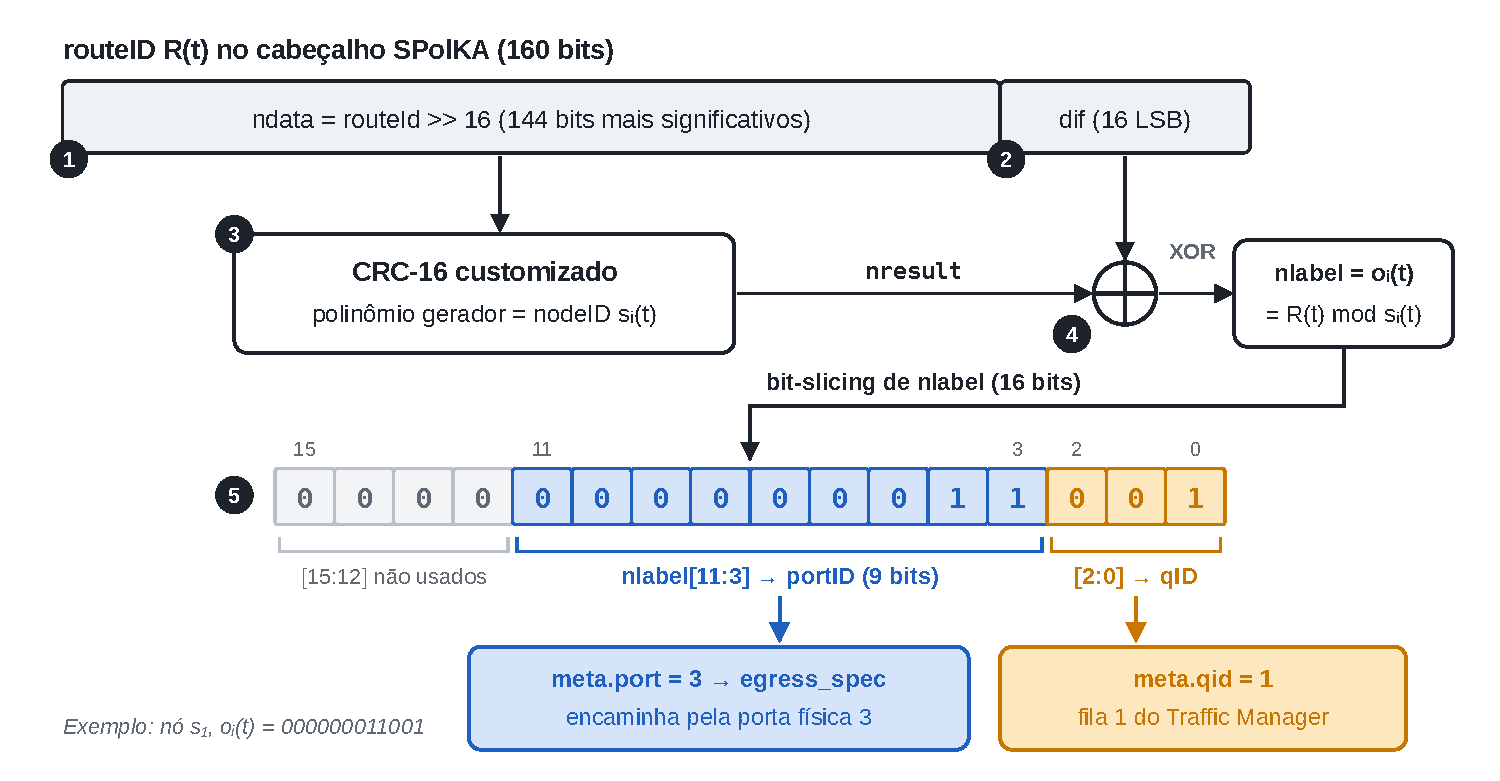
\includegraphics[width=\textwidth]{figuras/fig_a_decodificacao_spolka.pdf}
    \captionsetup{justification=centering}
    \caption{Fluxo de decodificação aritmética e fatiamento de bits (\textit{bit-slicing}) no plano de dados do \nome.}
    \label{fig:decodificacao_spolka}
\end{figure}

O fluxo completo dessa decodificação aritmética no pipeline de ingresso (\textit{Ingress}) de um comutador de núcleo é ilustrado na Figura~\ref{fig:decodificacao_spolka} e detalhado na implementação em linguagem P4 apresentada no Quadro~\ref{quad:codigo_controle}. Inicialmente, o cabeçalho de $160$ bits (\texttt{meta.routeId}) é particionado por meio de um deslocamento lógico de $16$ bits à direita para isolar os $144$ bits mais significativos (\texttt{ndata}, Etapa 1) e de um truncamento direto para extrair os $16$ bits menos significativos (\texttt{dif}, Etapa 2). Em seguida, a unidade de CRC-16 customizada calcula o resto polinomial \texttt{nresult} utilizando o \nodeID\ local como polinômio gerador (Etapa 3), o qual é combinado via operação \texttt{XOR} com \texttt{dif} para reconstituir o polinômio de saída $o_i(t)$ de $16$ bits (\texttt{nlabel}, Etapa 4).

Por fim, aplica-se o fatiamento de bits (\textit{bit-slicing}) sobre \texttt{nlabel} (Etapa 5): considerando uma palavra de controle útil de $12$ bits (com os bits $[15:12]$ reservados para expansões futuras), os $9$ bits intermediários (\texttt{nlabel[11:3]}) definem o identificador da porta física de saída (\portID, suportando até $512$ portas por comutador), enquanto os $3$ bits menos significativos (\texttt{nlabel[2:0]}) especificam o identificador da fila de serviço (\qID, endereçando até $8$ filas distintas por interface). No exemplo da Figura~\ref{fig:decodificacao_spolka}, para o nó $S_1$ com $o_1(t) = 000000011001$, a extração resulta em $\texttt{meta.port} = 3$ e $\texttt{meta.qid} = 1$, direcionando o pacote à fila prioritária $1$ da porta física $3$.

\begin{quadro}[htb]
    \centering
    \caption{Função de cálculo do rótulo SPolKA em linguagem P4}
    \label{quad:codigo_controle}
    \begin{lstlisting}[language=P4]
        action srcRoute_nhop() {
            bit<16> nresult;
    
            // 1. Extração dos 144 bits mais significativos do routeId por deslocamento à direita
            bit<160> ndata = meta.routeId >> 16;
            
            // 2. Truncamento direto para obtenção dos 16 bits menos significativos (termo independente)
            bit<16> dif = (bit<16>)meta.routeId;
    
            // 3. Cálculo do resto da divisão polinomial em GF(2) via unidade de CRC-16 customizado,
            // utilizando constantes literais para otimizar a alocação de registradores
            hash(nresult,
                 HashAlgorithm.crc16_custom,
                 16w0,           // Valor base (offset) nulo
                 {ndata}, 
                 64w8589934592); // Limite superior do domínio de saída (2^33)
    
            // 4. Composição do polinômio de saída o_i(t) via adição modular (XOR)
            bit<16> nlabel = nresult ^ dif;
    
            // 5. Fatiamento de bits (bit-slicing) para decodificação simultânea de encaminhamento e QoS:
            meta.port = (bit<9>)nlabel[11:3]; // Bits [11:3] determinam o identificador da porta de saída (portID)
            meta.qid  = (bit<3>)nlabel[2:0];  // Bits [2:0] especificam o identificador da fila de serviço (qID)
        }
    \end{lstlisting}
    \fonte{Elaborado pelo autor (2026), adaptado de \textcite{nerds_polka}.}
\end{quadro}

% ==============================================================================
\section{Escalonamento Programável e Gerenciamento de Tráfego}
\label{sec:traffic_manager}

A decodificação simultânea do \portID\ e do \qID\ no pipeline de ingresso somente se traduz em isolamento efetivo de QoS quando acoplada a um mecanismo de enfileiramento capaz de impor garantias de largura de banda e evitar a inanição (\textit{starvation}) de fluxos menos prioritários. Enquanto switches de hardware comerciais (como a família Intel Tofino) dispõem de gerenciadores de tráfego nativos configuráveis com algoritmos ponderados, e sistemas operacionais como o Linux oferecem disciplinas de enfileiramento nativas no subsistema \textit{Traffic Control} (\texttt{tc}), ambientes de emulação programável como o \textit{Behavioral Model version 2} (BMv2) implementam originalmente apenas escalonamento por prioridade estrita, no qual filas de menor precedência podem ser completamente bloqueadas sob condições de saturação.

Para superar essa limitação do escalonador nativo do BMv2 e alinhar o comportamento do plano de dados ao requisito \textbf{RF04}, a arquitetura do \nome\ integra um Gerenciador de Tráfego (\textit{Traffic Manager} -- TM) programável acoplado ao final do pipeline de \textit{Ingress}, conforme ilustrado na Figura~\ref{fig:traffic_manager}. Essa solução baseia-se na implementação de referência de escalonadores baseados em classificação em P4 proposta por \textcite{Elbediwy2025}, cujo código-fonte original, por ter sido concebido especificamente para o cenário de avaliação de seu próprio laboratório, apresentava acoplamento rígido às estruturas de cabeçalho e às condições experimentais daquele ambiente. No âmbito deste trabalho, o código em C++ da extensão externa (\textit{extern} \texttt{my\_scheduler}) foi refatorado e generalizado para operar de forma agnóstica aos protocolos encapsulados, permitindo que o algoritmo \textit{Weighted Deficit Round-Robin} (WDRR) seja aplicado a qualquer fluxo de tráfego interceptado após a execução da ação \texttt{srcRoute\_nhop()}.

\begin{figure}[!htb]
    \centering
    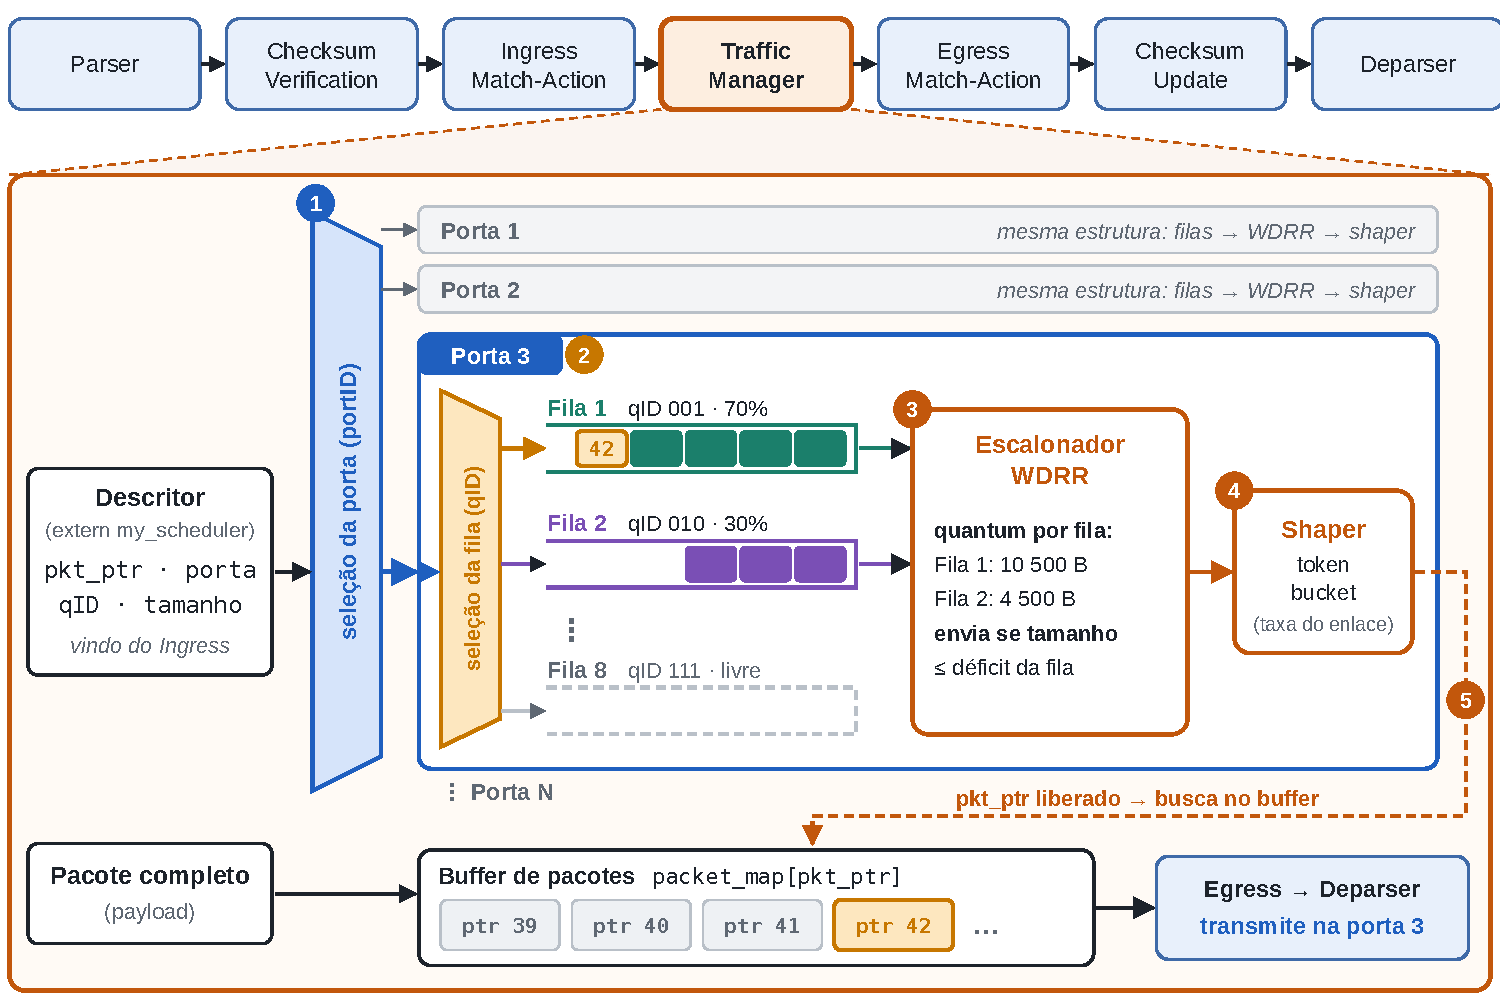
\includegraphics[width=\textwidth]{figuras/fig_b_traffic_manager.pdf}
    \captionsetup{justification=centering}
    \caption{Arquitetura interna do Gerenciador de Tráfego (\textit{Traffic Manager}) programável com escalonamento WDRR e \textit{shaping} por interface.}
    \label{fig:traffic_manager}
\end{figure}

O ciclo de enfileiramento e transmissão no \textit{Traffic Manager} ocorre em cinco etapas coordenadas, destacadas na Figura~\ref{fig:traffic_manager}:
\begin{enumerate}
    \item \textbf{Transferência do Descritor e Armazenamento em Buffer:} Ao concluir o processamento de \textit{Ingress}, o pacote completo (\textit{payload} e cabeçalhos) é armazenado em um buffer compartilhado indexado por um ponteiro único (\texttt{packet\_map[pkt\_ptr]}), enquanto um descritor compacto contendo o ponteiro (\texttt{pkt\_ptr}), a porta de destino (\texttt{portID}), o identificador da fila (\texttt{qID}) e o tamanho do quadro em bytes é repassado ao módulo escalonador.
    \item \textbf{Demultiplexação por Porta e Fila:} Com base no par $(\texttt{portID}, \texttt{qID})$ decodificado a partir do \routeID, o descritor é inserido na estrutura de filas correspondente à interface física de saída (e.g., Porta $3$, Fila $1$ para \texttt{qID = 001} ou Fila $2$ para \texttt{qID = 010}). Cada interface física mantém até $8$ filas lógicas isoladas, suportando tanto fatias com reservas garantidas quanto fatias de melhor esforço (\texttt{qID = 111}).
    \item \textbf{Escalonamento Ponderado via WDRR:} Para arbitrar a ordem de serviço entre as filas ativas de uma mesma porta sem incorrer em inanição, emprega-se o algoritmo \textit{Weighted Deficit Round-Robin} (WDRR). A cada rodada, cada fila não vazia recebe um crédito (\textit{quantum}) em bytes proporcional ao peso da fatia configurada (por exemplo, $10.500\text{ B}$ para a Fila $1$ com reserva de $70\%$ e $4.500\text{ B}$ para a Fila $2$ com reserva de $30\%$). Um pacote somente é desenfileirado se o seu tamanho em bytes for inferior ou igual ao déficit acumulado da respectiva fila; caso contrário, o saldo remanescente é preservado para a rodada subsequente. Além de assegurar o isolamento estrito sob congestionamento, o WDRR permite que uma fatia utilize a banda ociosa de filas inativas, maximizando a eficiência estatística do enlace.
    \item \textbf{Modelagem de Taxa (\textit{Shaping}):} Os descritores selecionados pelo escalonador WDRR passam por um regulador baseado em balde de fichas (\textit{token bucket shaper}), responsável por limitar a taxa de transmissão agregada à capacidade nominal do enlace físico e absorver micro-rajadas de tráfego.
    \item \textbf{Recuperação e Transmissão no Egresso:} Uma vez autorizado pelo \textit{shaper}, o descritor libera o ponteiro \texttt{pkt\_ptr}, permitindo que o pacote original seja recuperado do \texttt{packet\_map}, processado pelo pipeline de \textit{Egress} e pelo \textit{Deparser}, e finalmente transmitido pela interface física de saída.
\end{enumerate}

% ==============================================================================
\section{Reconfiguração Dinâmica e Migração Ágil de Fatias}
\label{sec:migracao_agil}

% Uma das principais vantagens arquiteturais do \nome\ frente aos modelos tradicionais de engenharia de tráfego e fatiamento (tais como MPLS-TE, RSVP-TE ou DiffServ acoplado a roteamento hop-by-hop) reside na agilidade de reconfiguração e na ausência de tempo de convergência no núcleo da rede.

% Em cenários operacionais dinâmicos --- como a chegada repentina de tráfego concorrente em um enlace compartilhado, a degradação de métricas de latência ou a necessidade de promover uma fatia para uma classe de serviço superior ---, a modificação das garantias de QoS no \nome\

Como os comutadores de núcleo não mantêm estados por fluxo nem tabelas de mapeamento de fatias, a transição ocorre de maneira atômica e instantânea no plano de dados, sem perda de pacotes por inconsistência transitória de tabelas e sem sobrecarga de sinalização no plano de controle.

Para validar empiricamente os requisitos levantados e comprovar a eficácia da arquitetura \nome\ sob condições controladas e realistas, foram desenvolvidos dois protótipos complementares: (i) um ambiente emulado baseado em P4/BMv2, estendido com o gerenciador de tráfego programável com escalonamento ponderado (WDRR); e (ii) uma topologia virtualizada em \textit{Containerlab} sobre contêineres Ubuntu 24.04, na qual o processamento de pacotes do \nome\ é executado em eBPF/XDP integrado ao subsistema nativo de controle de tráfego (\texttt{tc}) do \textit{kernel} Linux. O Capítulo~\ref{chap:prototipos} detalha a implementação técnica desses protótipos --- abrangendo a programação dos planos de dados, a configuração dos escalonadores e a orquestração do plano de controle ---, bem como apresenta a metodologia experimental e a análise dos resultados obtidos em termos de isolamento de largura de banda, latência e agilidade na migração de fluxos.

% ---
% ------------------------ PROTÓTIPO ------------------
% ---

%\chapter{PROTÓTIPO}
\label{chap:prototipos}

Neste capítulo, apresentam-se três protótipos experimentais desenvolvidos com o propósito de avaliar e validar o fatiamento de rede (\textit{network slicing}) e a garantia de requisitos de Qualidade de Serviço (QoS) sob a ótica do sistema de numeração de resíduos (RNS, do inglês \textit{Residue Number System}). A abordagem adota uma estratégia incremental de validação, cobrindo diferentes níveis de fidelidade de hardware, flexibilidade de prototipagem e eficiência de encaminhamento:

\begin{enumerate}
    \item \textbf{Ambiente em hardware programável (Tofino/freeRtr):} topologia interestadual com enlaces de 10~Gbps e comutadores baseados no circuito integrado Intel Tofino\textregistered, operando sob o \textit{framework} freeRtr, com o objetivo de atestar a capacidade da arquitetura PolKA original em prover garantias de QoS estritamente por meio da seleção de caminhos fim a fim;
    \item \textbf{Ambiente comportamental P4 (BMv2/Mininet):} implementação concebida para validar as extensões da arquitetura SPolKA (\textit{Service PolKA}), elevando a granularidade do fatiamento ao codificar a rota de encaminhamento e a classe de escalonamento em um único rótulo no cabeçalho;
    \item \textbf{Ambiente baseado em contêineres e SO programável (Containerlab/eBPF):} infraestrutura leve orquestrada sobre contêineres Ubuntu, empregando eBPF (\textit{Extended Berkeley Packet Filter}) no plano de dados para executar o encapsulamento, a manipulação de rótulos e o encaminhamento eficiente dos pacotes em ambiente de rede virtualizada.
\end{enumerate}

A coexistência dessas três frentes experimentais fundamenta-se nas características e restrições de cada ecossistema. As operações de plano de dados introduzidas pelo SPolKA preservam a mesma base aritmética do PolKA tradicional, cuja viabilidade em taxa de linha já foi previamente validada em hardware Tofino por \cite{dominicini2021}. Contudo, como o \textit{framework} de controle freeRtr ainda não contempla nativamente as extensões de cabeçalho necessárias para o SPolKA, optou-se pela implementação comportamental em switches BMv2 sobre o emulador Mininet.

Para contornar o problema de inanição (\textit{starvation}) decorrente da política de prioridade estrita (\textit{Strict Priority}) nativa do BMv2, aprimorou-se a arquitetura de enfileiramento com o algoritmo \textit{Weighted Deficit Round-Robin} (WDRR), distribuindo a largura de banda de forma proporcional aos pesos atribuídos a cada fatia. Fundamentando-se na abordagem proposta por \cite{Elbediwy2025}, integrou-se um \textit{Traffic Manager} (TM) customizado em C++ por meio de \textit{software externs}, transferindo os pacotes ao módulo de gerenciamento de tráfego ao término do estágio de \textit{Ingress}. Com isso, o comportamento do ambiente emulado aproxima-se com fidelidade da dinâmica de comutadores de produção.

No plano de controle e borda da rede (\textit{ingress edge}), a classificação de tráfego utiliza o campo DSCP (\textit{Differentiated Services Code Point}) do modelo DiffServ para derivar o mapeamento conjunto de fluxos, rotas e classes de serviço em um identificador único denominado \texttt{routeID} --- prevendo-se, para trabalhos futuros, a adoção dos parâmetros SST (\textit{Slice/Service Type}) e SD (\textit{Slice Differentiator}) do padrão S-NSSAI da arquitetura 5G/6G. 

No núcleo da rede (\textit{core}), o cálculo dos módulos de resíduos em taxa de linha supera as restrições inerentes da linguagem P4 ao reaproveitar os motores de hardware de CRC. Conforme demonstrado na análise de escalabilidade de \cite{dominicini2020}, a sobrecarga de cabeçalho do \texttt{routeID} é determinada pelo produto do diâmetro máximo da topologia (em saltos) por 2~bytes (CRC-16 com suporte a até 4.080 nós de núcleo). Neste trabalho, definiu-se um limite superior de 10 saltos, resultando em um cabeçalho \texttt{routeID} de 20~bytes, particionado conceitualmente para acomodar identificadores de porta de saída (\texttt{portID}) de 13~bits e identificadores de fila (\texttt{qID}) de 3~bits, viabilizando o isolamento de até 8 filas por interface.

O principal diferencial do SPolKA reside na flexibilidade de adaptação: alterações dinâmicas de trajetos e políticas de escalonamento são efetuadas exclusivamente pela reconfiguração pontual do rótulo na borda, mantendo o núcleo da rede totalmente sem estado (\textit{stateless}). 

Nas seções seguintes, detalham-se os requisitos, a topologia, o fluxo de execução e a instrumentação metodológica empregada em cada um dos protótipos desenvolvidos.


----

Neste capítulo, apresentam-se três protótipos desenvolvidos para mitigar o 
desafio de assegurar os requisitos de Qualidade de Serviço (QoS) para distintas 
classes de serviço. O primeiro protótipo consiste em um ambiente experimental que 
emula uma rede interestadual composta por enlaces de 10~Gbps e comutadores 
baseados no circuito integrado Intel Tofino\textregistered. O segundo cenário 
foi concebido no ambiente de emulação Mininet, utilizando switches de software 
baseados na arquitetura comportamental BMv2. Por fim, o terceiro protótipo 
foi implementado a partir de contêineres Ubuntu orquestrados via Containerlab, 
empregando eBPF para a realização do encapsulamento e do encaminhamento 
eficiente dos pacotes.

Para validar a eficácia do fatiamento baseado em RNS, desenvolveram-se três protótipos complementares. O primeiro, em hardware Tofino sob o framework freeRtr\footnote{\url{http://www.freertr.org/}}, atesta a capacidade do \polka original em prover QoS apenas pela seleção de caminhos fim a fim. O segundo foca no \spolka, elevando a granularidade ao codificar rota e escalonamento em um único rótulo. As operações no plano de dados do \spolka são as mesmas do \polka original, que já foi validado em hardware Tofino \cite{dominicini2021}. Para este trabalho, a solução foi implementar o \spolka no switch de software BMv2 (emulado no Mininet), pois o framework freeRtr ainda não suporta as extensões de cabeçalho do \spolka. Para superar a inanição causada pela prioridade estrita nativa do BMv2, aprimorou-se a arquitetura com o algoritmo Weighted Deficit Round-Robin (WDRR), que distribui a banda proporcionalmente aos pesos das fatias \cite{Elbediwy2025}. Baseando-se em \textcite{Elbediwy2025}\footnote{\url{https://github.com/Elbediwy/DR-PIFO_hierarchical_TM_SW.git}}, integrou-se um Traffic Manager (TM) customizado em C++ via software externs, que transferem os pacotes ao TM no final do pipeline de Ingress. Isso alinha a emulação ao comportamento de hardwares de produção (como o Tofino).

Na borda, a classificação usa o campo DSCP (\textit{Differentiated Services Code Point}) do \textit{DiffServ} para mapear fluxos em rotas e classes de serviço num único \routeID. Em trabalhos futuros, planeja-se adotar os parâmetros SST (\textit{Slice/Service Type}) e SD (\textit{Slice Differentiator}) do identificador S-NSSAI. No núcleo, a operação de módulo em taxa de linha contorna as restrições matemáticas do P4 reusando o hardware de CRC. Conforme detalhado na análise de escalabilidade em \cite{dominicini2020}, o tamanho do cabeçalho do \routeID é dado pela multiplicação do número máximo de saltos da topologia por 2 bytes (CRC16 com até 4.080 nós de núcleo). Neste trabalho, adotou-se o número máximo de 10 saltos, um \routeID de 20 bytes, um portID de 13 bits e um \qID de 3 bits (8 filas). O diferencial do \spolka é a migração ágil de rotas e políticas de filas, alterando apenas um rótulo na borda, sem reconfigurar o núcleo. Os experimentos evidenciam como essa adaptação dinâmica torna o \spolka particularmente eficaz para o fatiamento de redes.

\section{PROTÓTIPO 1 - \polka original: Fatiamento com seleção de caminhos}

A topologia PORVIR (Figura \ref{fig:porvir_rede}) é composta por quatro nós implementados em switches programáveis Tofino. Para avaliar individualmente os caminhos, configuraram se três túneis \polka. Inicialmente, caracterizou-se o desempenho de cada caminho da rede em termos de latência, vazão média e retransmissões, conforme a Tabela 3a. As medições de tráfego TCP ocorreram via iperf3 por 60 minutos para cada caminho, com amostragens a cada 30 s. Adicionalmente, o tempo de resposta médio (RTT) foi aferido com a ferramenta ping (amostras de 1 s) por 60 minutos. Os resultados mostram que o caminho VIX–RJ–SP apresenta desempenho significativamente superior, com vazão 46 vezes maior, menor atraso e menos retransmissões.

\begin{figure}[htbp]
\centering
\captionsetup{justification=centering}

    \begin{subfigure}[b]{0.41\linewidth}
        \centering
        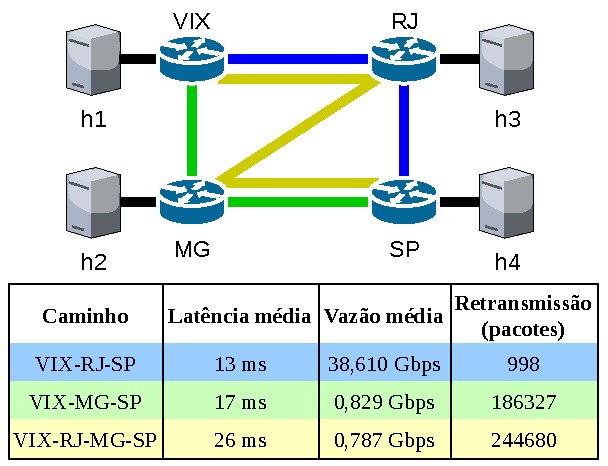
\includegraphics[width=\linewidth]{figuras/Porvir - Tabela e Topo.pdf}
        \caption{Métricas por caminho.}
        \label{fig:porvir_rede}
    \end{subfigure}
    \hfill
    \begin{subfigure}[b]{0.57\linewidth}
        \centering
        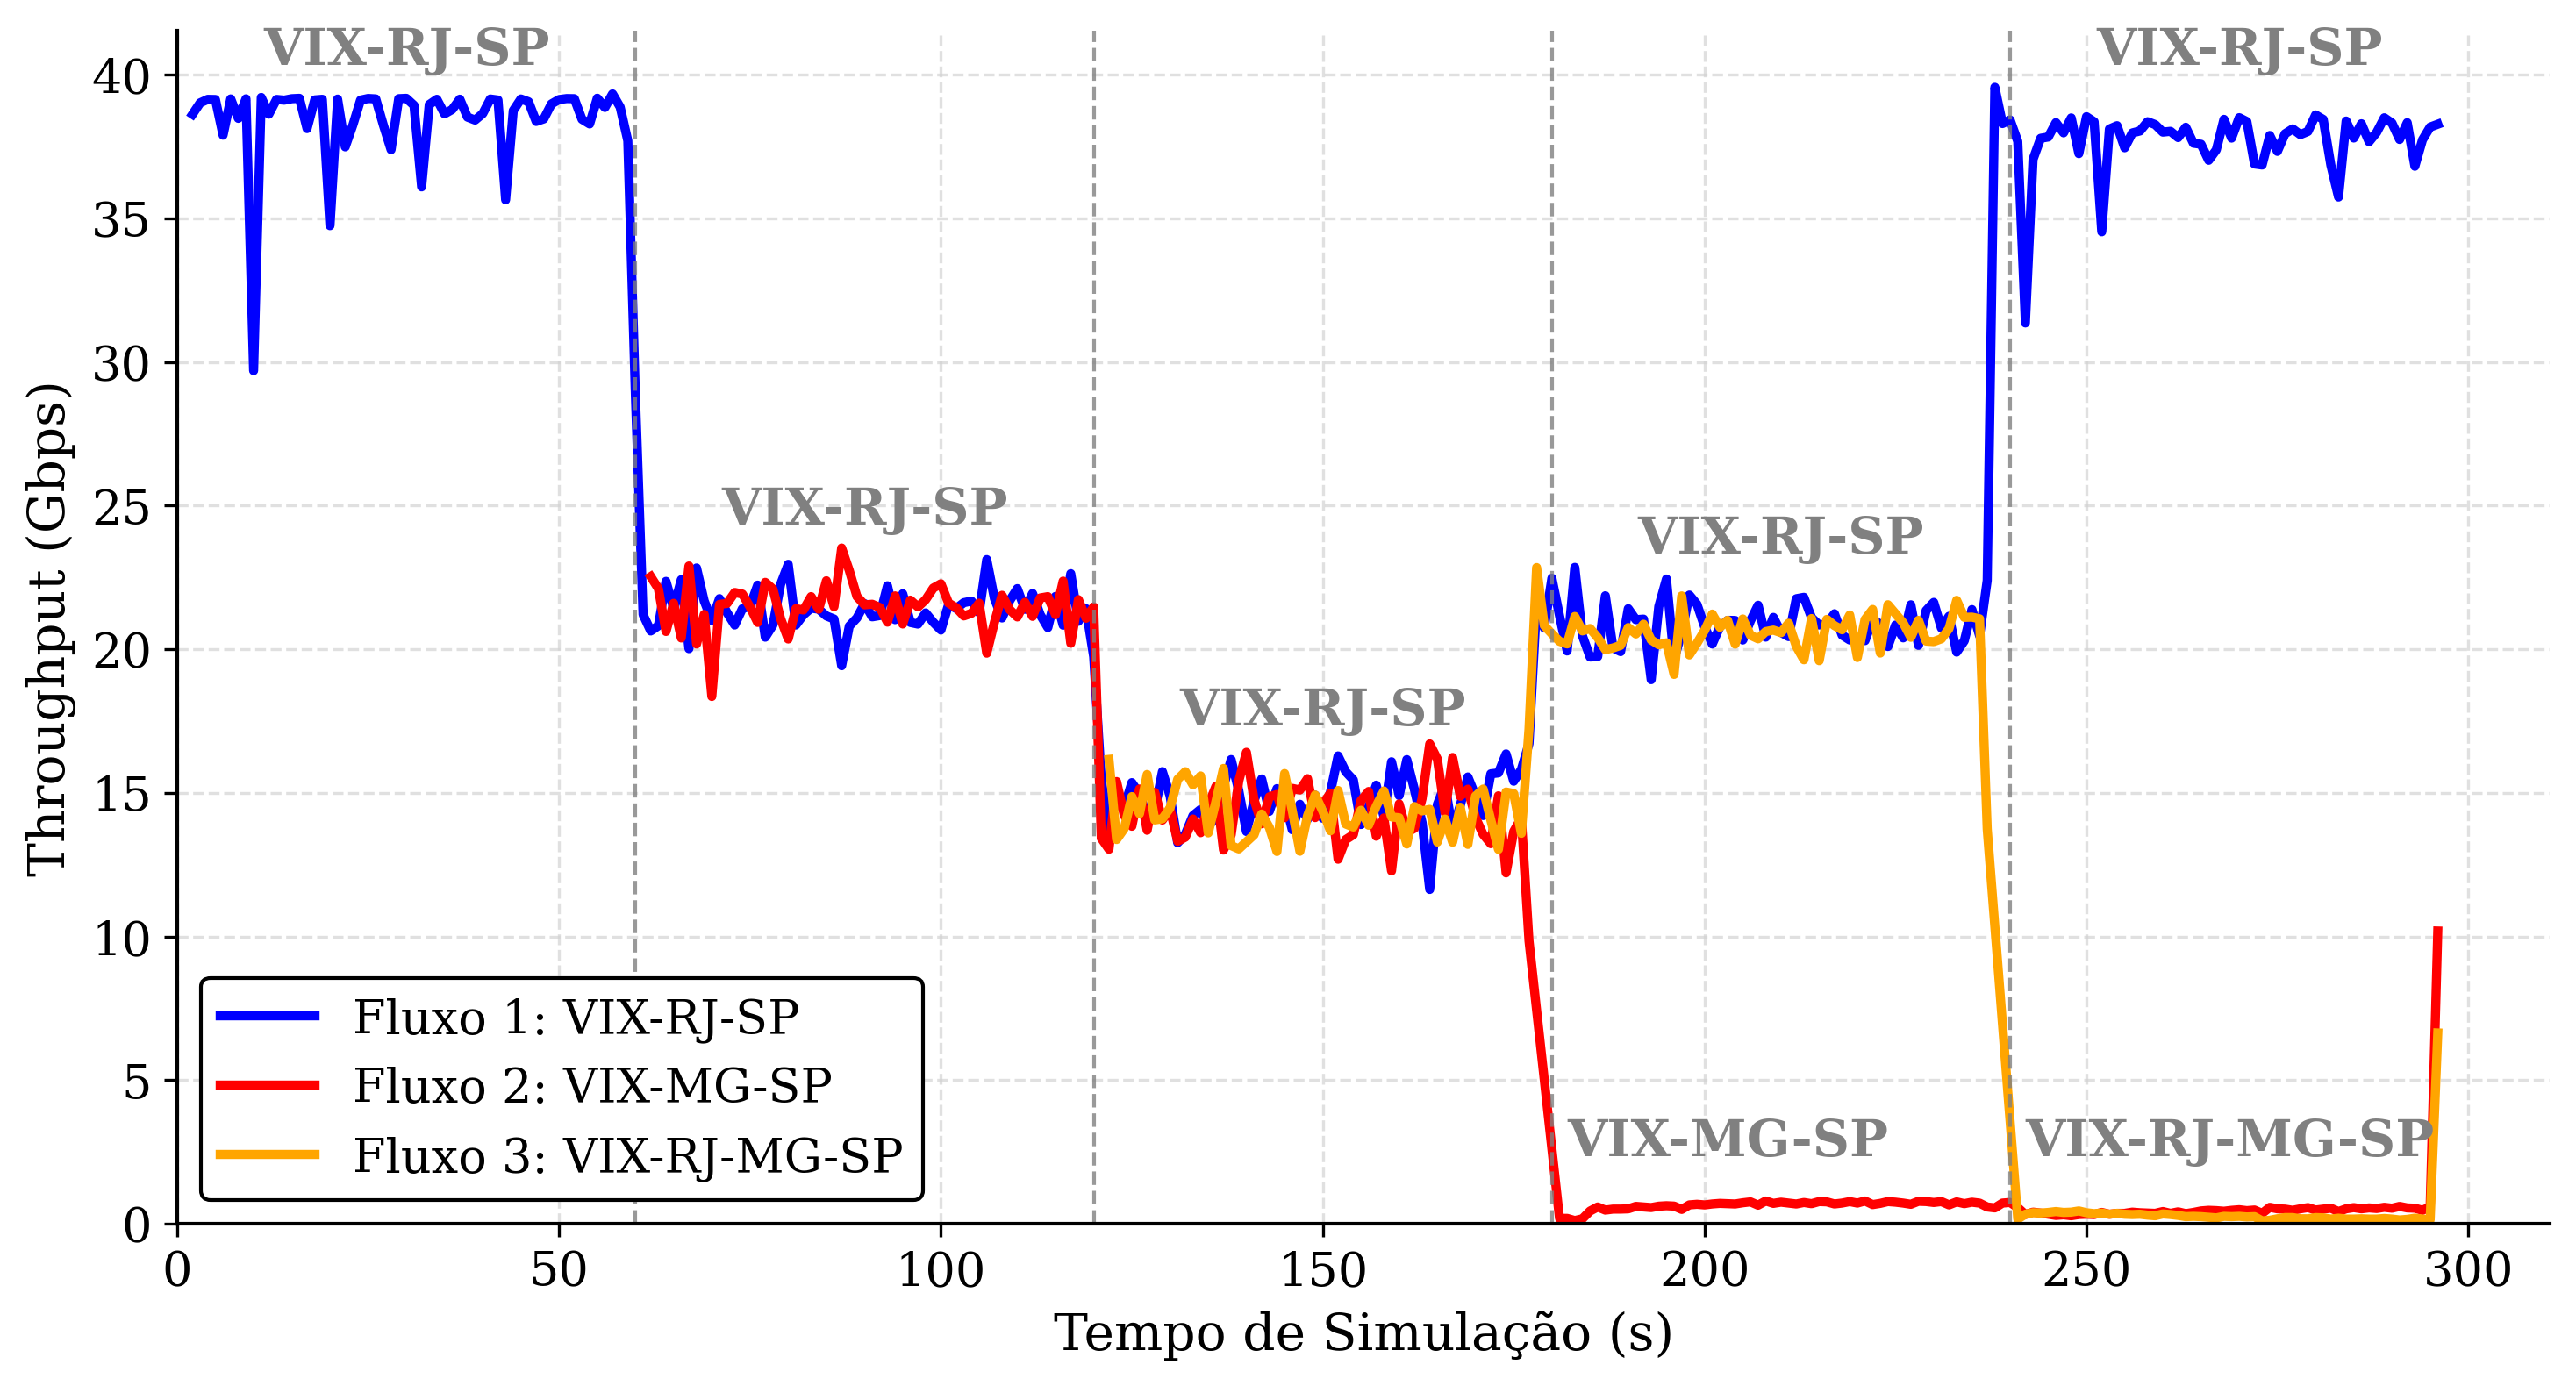
\includegraphics[width=\linewidth]{figuras/grafico_mudanca_caminho_porvir.png}
        \caption{Mudança de caminho.}
        \label{fig:mudanca_caminho_fila}
    \end{subfigure}

\caption{Resultados dos experimentos no testbed nacional Porvir.}
\label{fig:matriz_resultados}
\end{figure}

Após a caracterização, um experimento com três fluxos TCP (via iperf3) no enlace de alta capacidade (VIX–RJ–SP) representou a coexistência de um tráfego de maior prioridade com tráfegos de menor prioridade. Nesse cenário, cada fluxo atua como uma fatia de rede independente, que recebe recursos isolados e é configurada dinamicamente conforme seus requisitos específicos de \textit{QoS}. A figura \ref{fig:mudanca_caminho_fila} apresenta a vazão coletada ao longo dos eventos, espaçados a cada 60 s. Na fase de competição (0–180 s), a fatia do Fluxo 1 inicia isolada no caminho principal. Aos 60 s e 120 s, as fatias dos Fluxos 2 e 3 são ativadas na mesma rota, compartilhando a banda do enlace. Na fase de migração (180–300 s), evidenciando o isolamento e a adaptação dinâmica, as fatias concorrentes são realocadas para rotas alternativas de menor capacidade: o Fluxo 2 para VIX–MG–SP (aos 180 s) e o Fluxo 3 para VIX–RJ–MG–SP (aos 240 s). Com isso, a fatia do Fluxo 1, mais prioritário, restabelece o uso integral do enlace principal.

\section{PROTÓTIPO 2 - \spolka\: Fatiamento com seleção de caminhos e políticas de filas}

O segundo protótipo foi avaliado em dois cenários de acordo com a topologia da Figura \ref{fig:topologia_polka}: no primeiro, investigou-se exclusivamente o impacto da alteração das políticas de filas, enquanto o segundo analisou a reconfiguração concomitante de rotas e filas. Os enlaces têm capacidades de 10~Mbps com duas filas de prioridade por interface em cada roteador: a \textit{Fila 1}, com reserva de 70\% da largura de banda, e a \textit{Fila 2}, com os 30\% remanescentes. Os fluxos de dados foram gerados usando \textit{iperf3} com protocolo TCP. % com uma vazão nominal de 10~Mbps.
\begin{figure}[htbp]
    \centering
    % --- COLUNA DA ESQUERDA (Imagem Grande) ---
    \begin{subfigure}[t]{0.48\textwidth}
        \centering
        \vspace{0pt} % Truque para forçar o alinhamento no topo
        \fbox{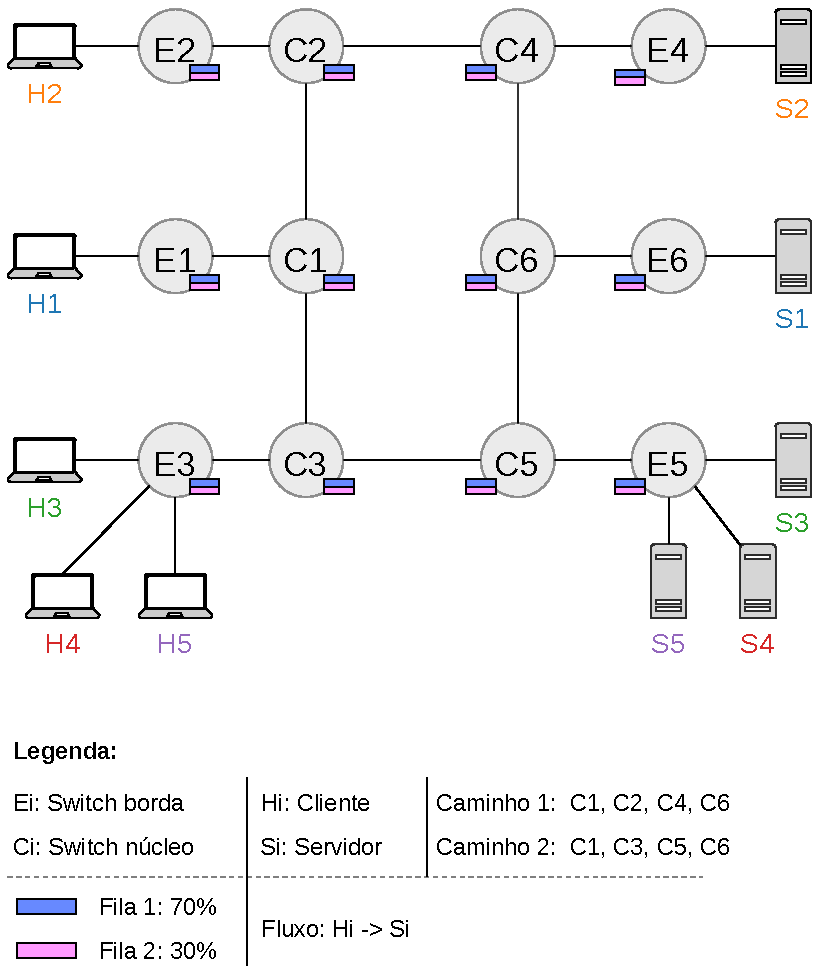
\includegraphics[width=\linewidth]{figuras/topologia - SBRC WPEIF 2026_v4.pdf}}
        \caption{Topologia da rede}
        \label{fig:topologia_polka}
    \end{subfigure}
    \hfill % Joga a outra coluna para o canto direito
    % --- COLUNA DA DIREITA (Duas Imagens Empilhadas) ---
    \begin{minipage}[t]{0.48\textwidth}
        \centering
        \vspace{0pt} % Garante que o topo da minipage alinhe com a esquerda
        
        \begin{subfigure}{\linewidth}
            \centering
            \fbox{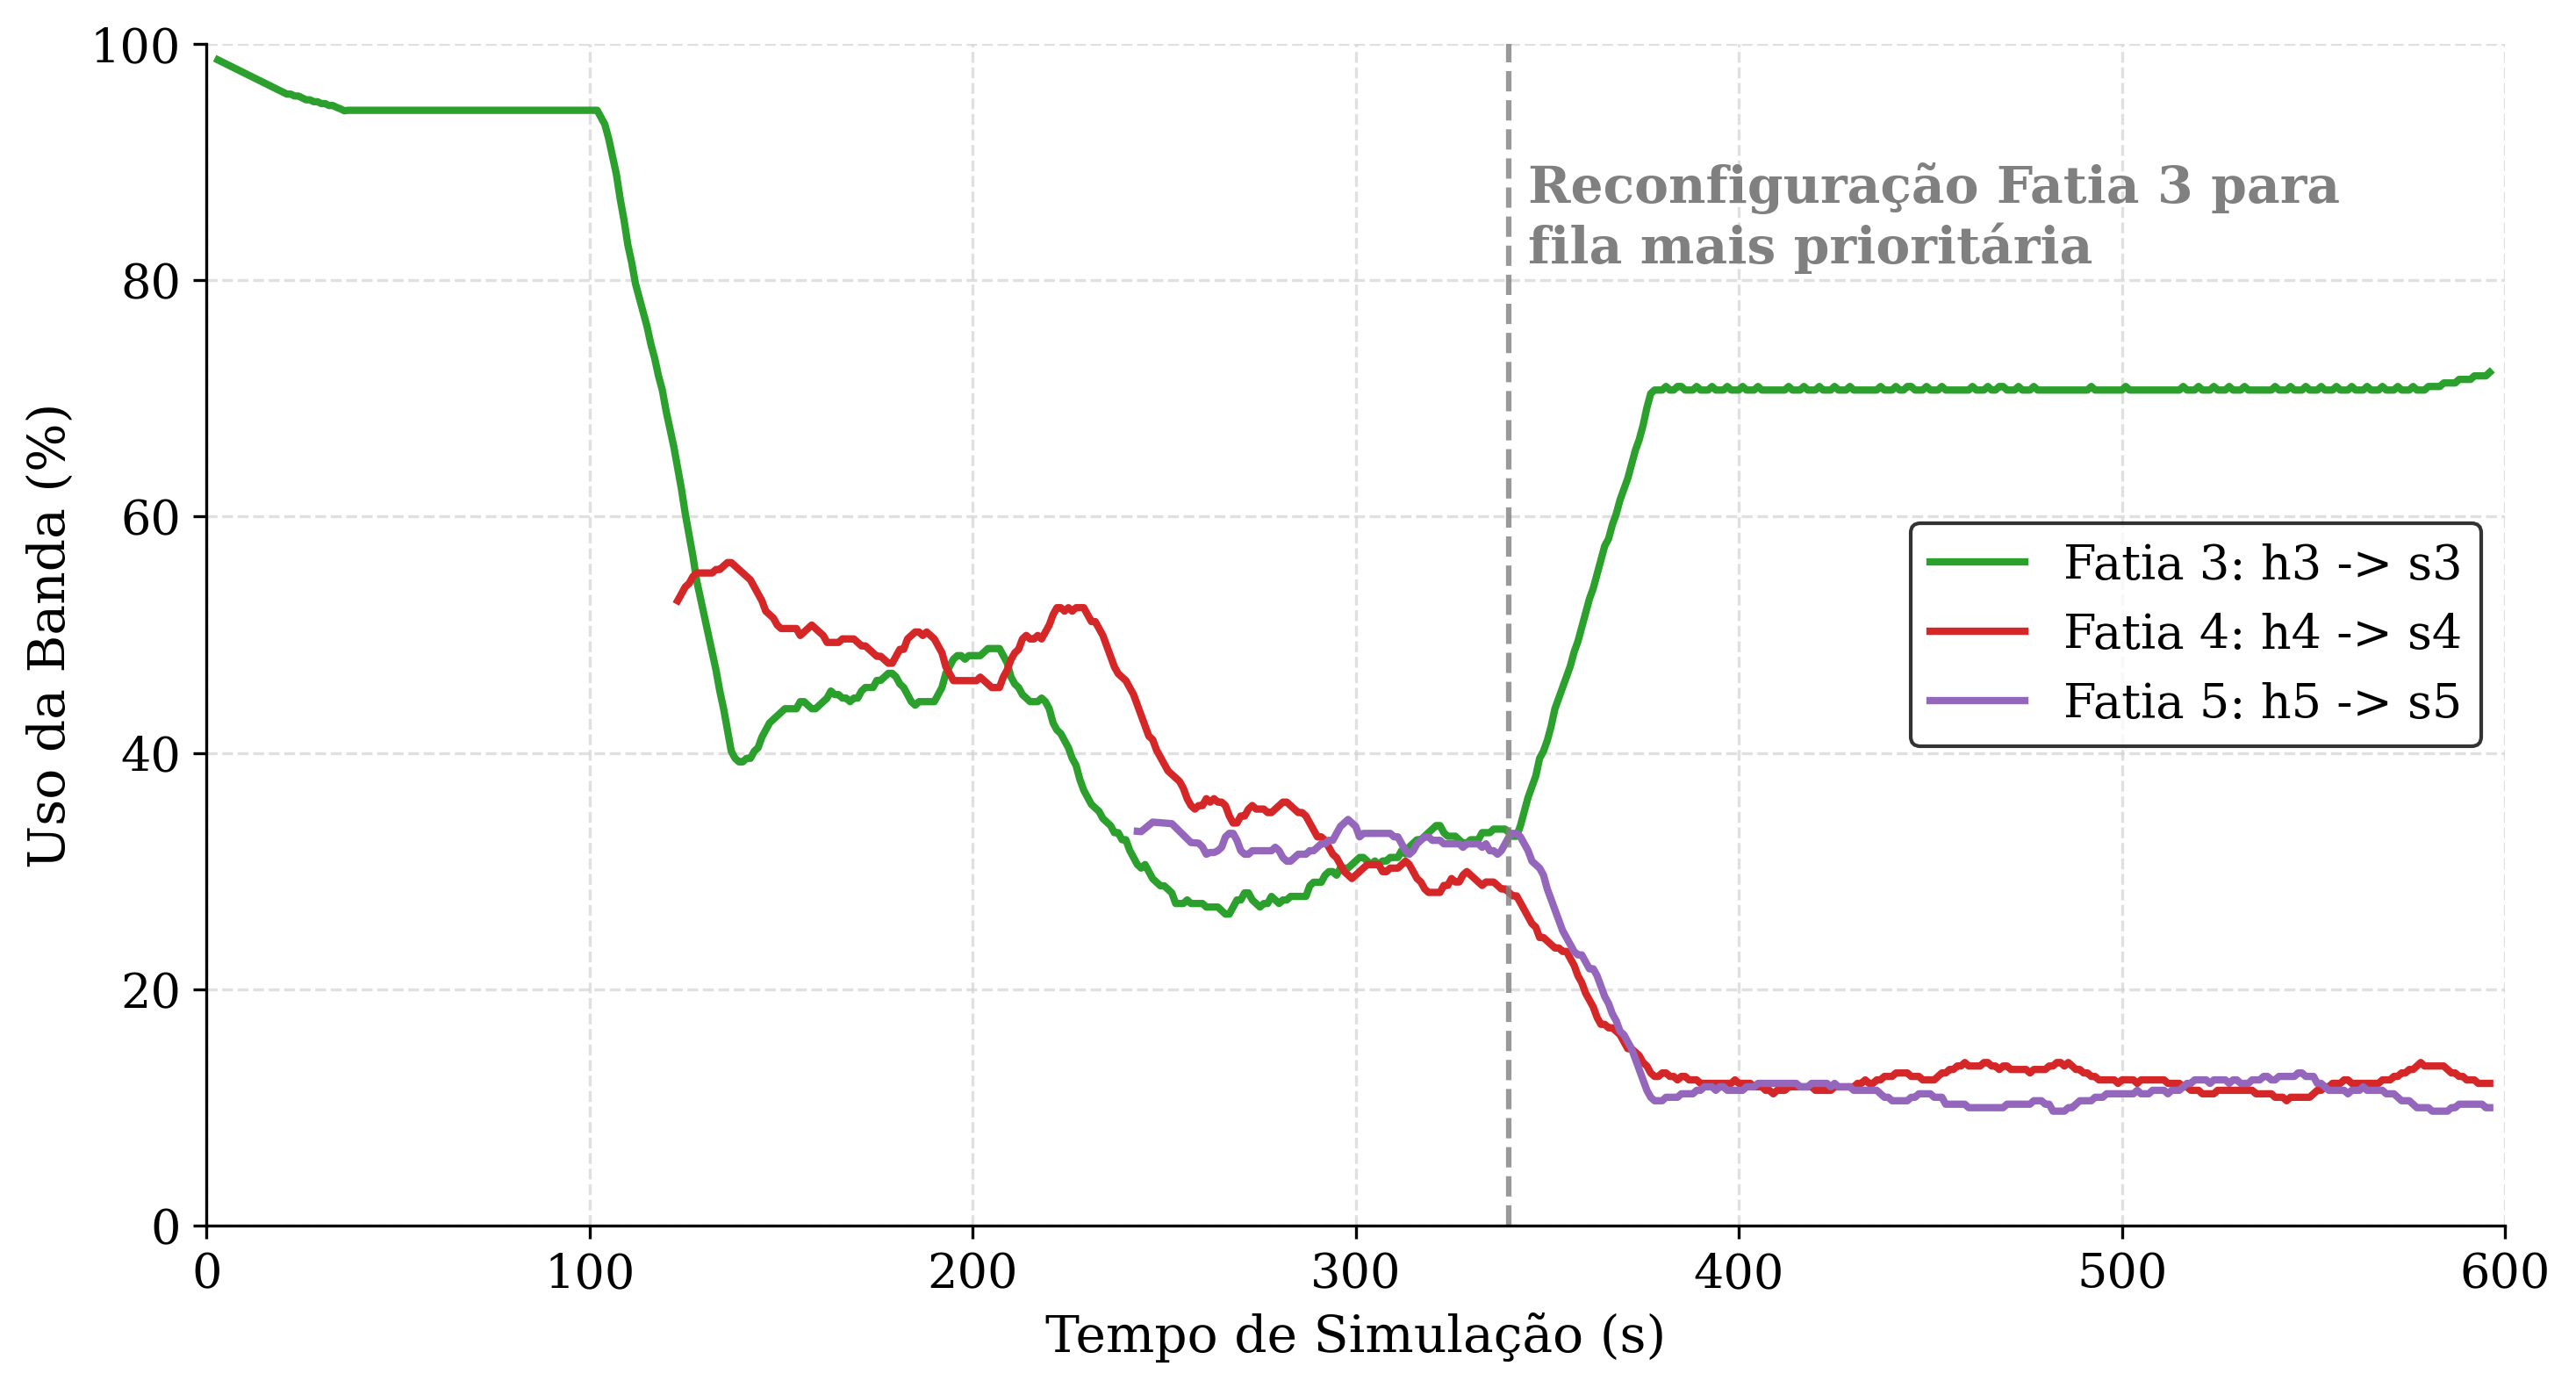
\includegraphics[width=\linewidth]{figuras/grafico_mudanca_fila_polka.png}}
            \caption{Mudança para fila prioritária}
            \label{fig:mininet_mudanca_fila_polka}
        \end{subfigure}
        
        % \vspace{1.0 cm} % Espaço entre as duas da direita
        
        \begin{subfigure}{\linewidth}
            \centering
            \fbox{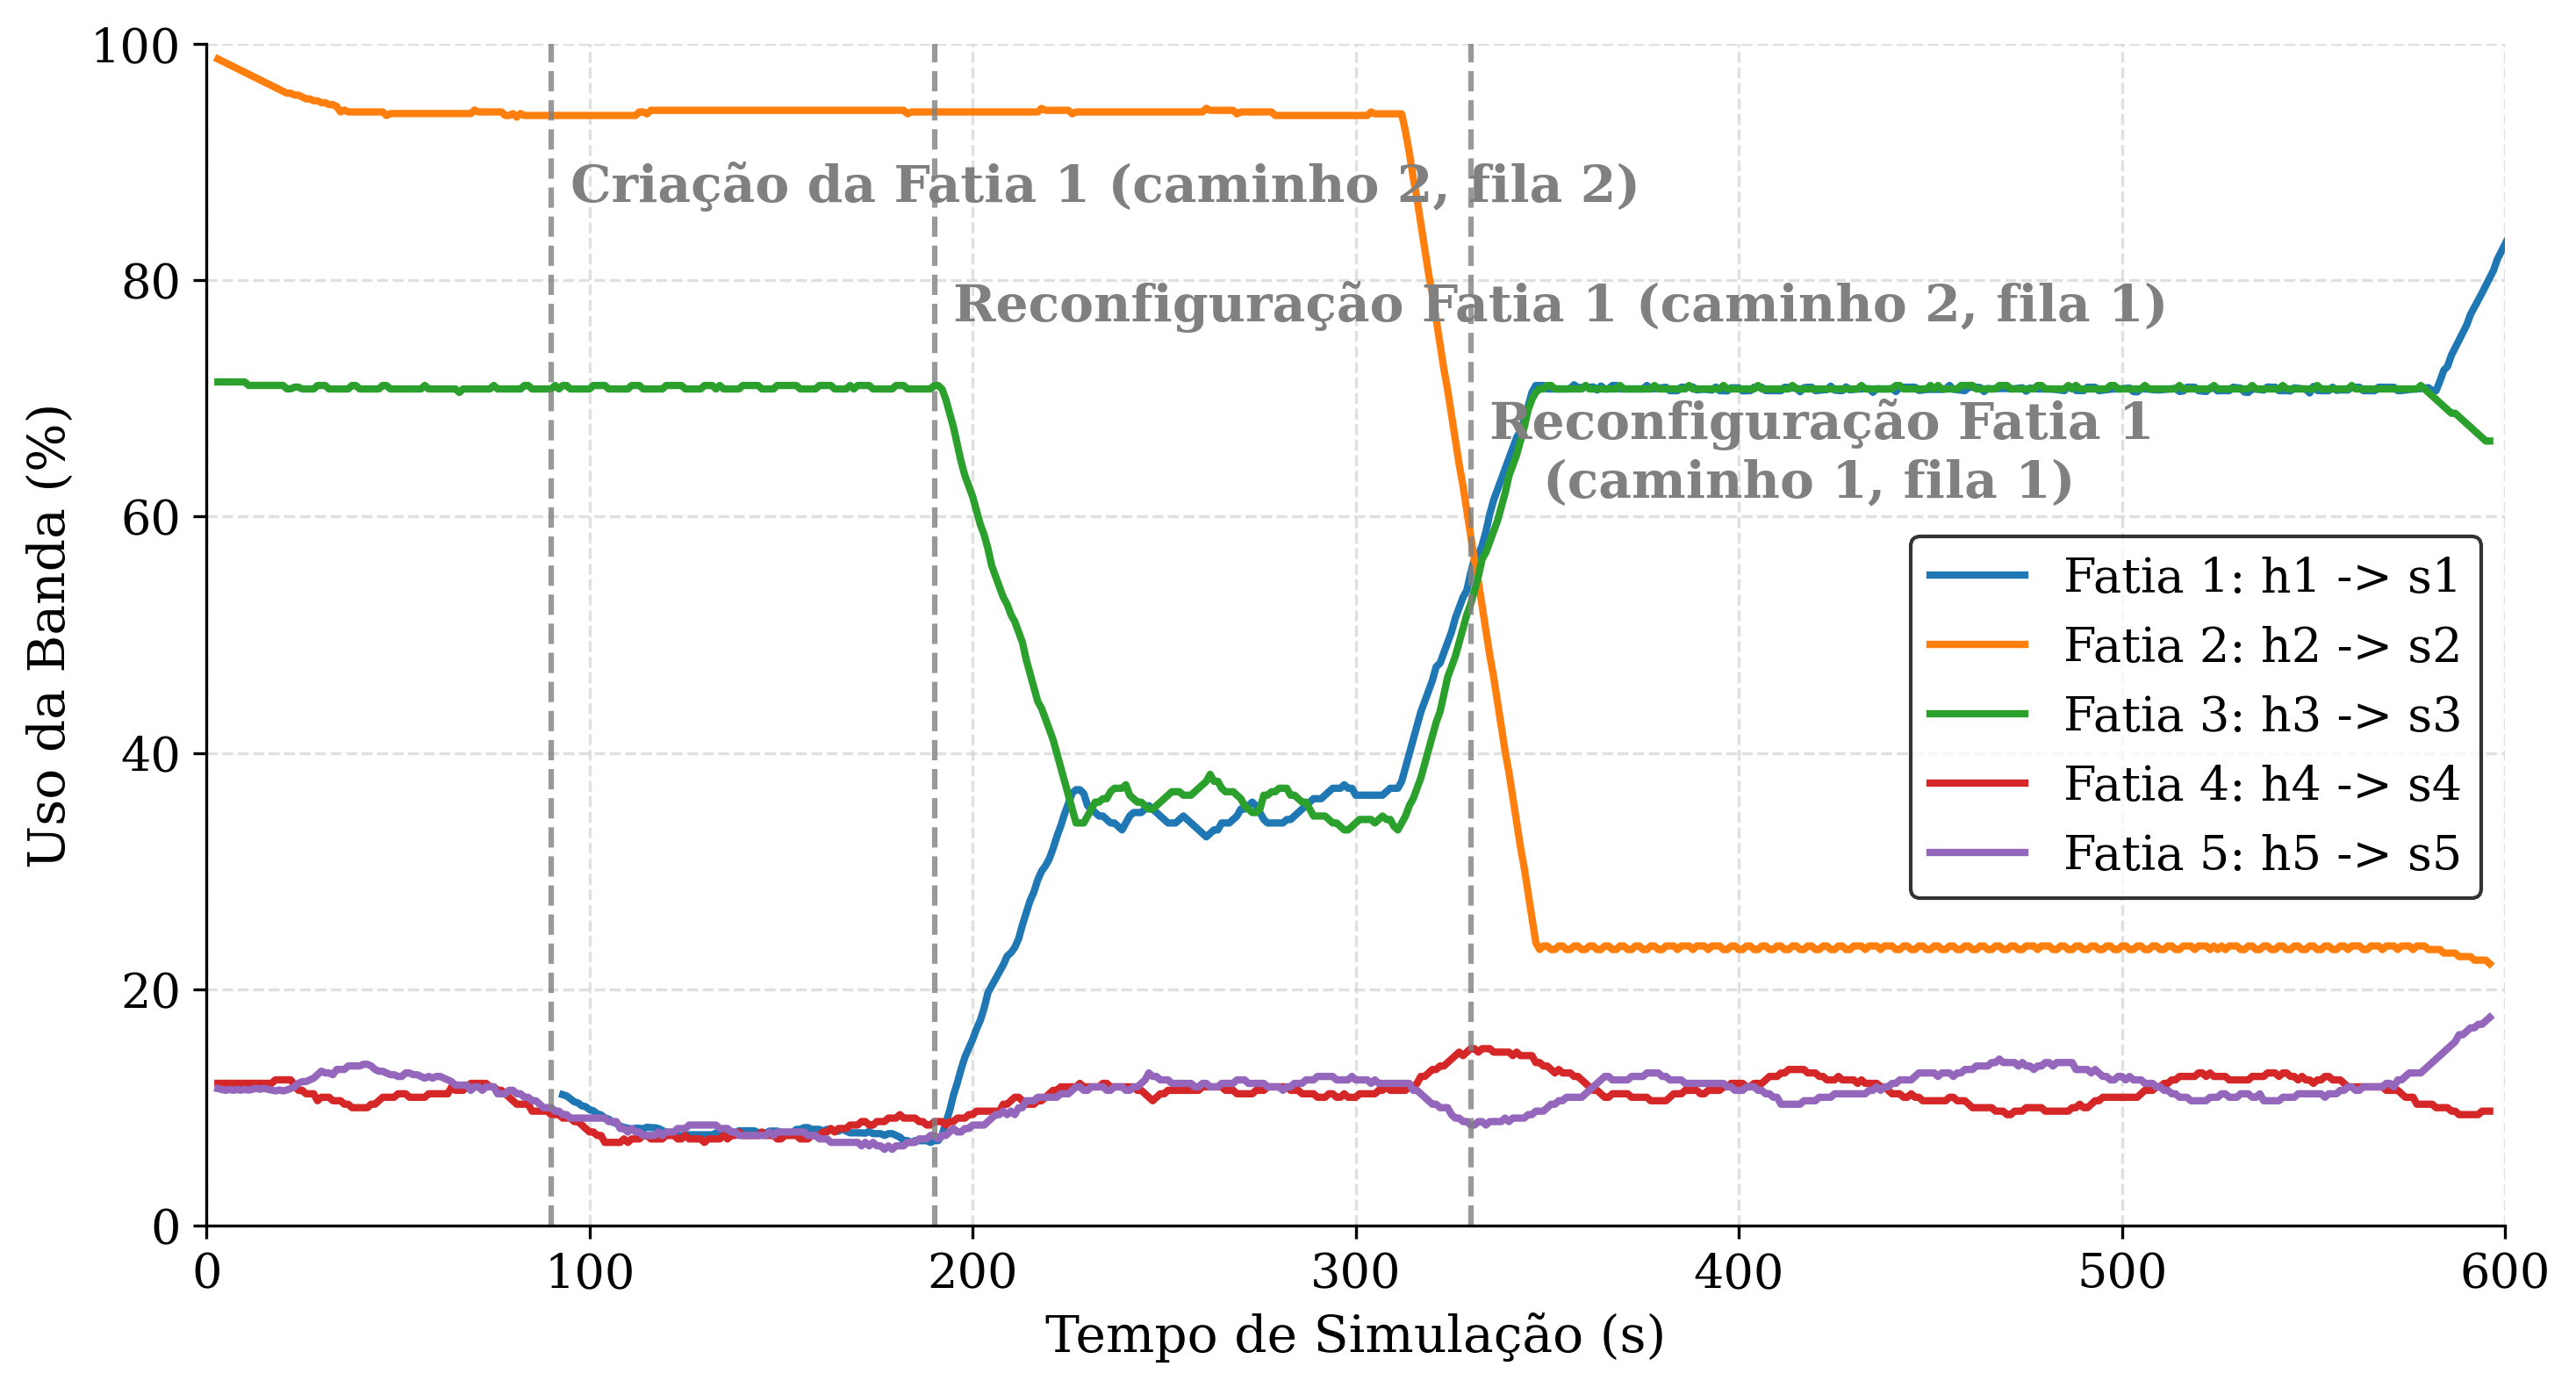
\includegraphics[width=\linewidth]{figuras/grafico_mudanca_caminho_fila_polka.png}}
            \caption{Mudança de caminho e fila}
            \label{fig:mininet_mudanca_caminho_fila}
        \end{subfigure}
    \end{minipage}

    \caption{Alteração de políticas de QoS para fatias de rede com SPolKA.}
    \label{fig:polka_combined}
\end{figure}

No primeiro cenário (Figura \ref{fig:mininet_mudanca_fila_polka}), analisou-se o desempenho de três fatias de rede encaminhadas pela rota $\{C_3, C_5\}$: uma fatia de alta prioridade, representada pelo fluxo $H_3 \rightarrow S_3$, e duas fatias de menor prioridade, representadas pelos fluxos $H_4 \rightarrow S_4$ e $H_5 \rightarrow S_5$. O objetivo foi validar a eficácia do isolamento e da priorização de recursos em condições de saturação de rede.
%
Em $t=0$~s, o fluxo $H_3 \rightarrow S_3$ foi alocado na \textit{Fila 2} em todos os saltos. 
A aplicação do algoritmo WDRR garante que, na ausência de fluxo na fila prioritária, a banda total disponível pode ser compartilhada entre as demais filas.
Posteriormente, em $t=90$~s e $t=180$~s, os fluxos $H_4 \rightarrow S_4$ e $H_5 \rightarrow S_5$ foram configurados, na mesma fila, resultando no compartilhamento equitativo da banda disponível entre as três fatias. 
%. Dado que os nós $C_3$ e $C_5$ constituem o caminho de convergência dos fluxos, a vazão disponível foi fragmentada proporcionalmente entre as três conexões ativas na Fila 2.
%
Finalmente, em $t=270$~s, procedeu-se à reconfiguração do fluxo $H_3 \rightarrow S_3$ para a \textit{Fila 1}, que possui uma reserva estrita de 70\% da largura de banda. Esta reconfiguração visou assegurar o isolamento de desempenho para o tráfego prioritário. Os fluxos remanescentes na Fila 2 (origem $H_4$ e $H_5$) passaram a competir pelos 30\% restantes da capacidade alocada, validando a capacidade do mecanismo de fatiamento em assegurar requisitos de QoS e mitigar interferências entre diferentes classes de serviço. 

% \subsection{Experimento 2 - mudança de caminho e fila}

O segundo cenário (Figura \ref{fig:mininet_mudanca_caminho_fila}) analisa o impacto da reconfiguração dinâmica concomitante de filas e rotas. % para a fatia representada pelo fluxo $H_1 \rightarrow S_1$. 
Em $t=0$~s, foi instanciada uma fatia de rede na rota $\{C_2, C_4\}$ referente ao fluxo $H_2 \rightarrow S_2$ e três fatias na rota $\{C_3, C_5\}$ referentes aos fluxos $H_3 \rightarrow S_3$, $H_4 \rightarrow S_4$ e $H_5 \rightarrow S_5$. A fatia com origem $H_2$ foi alocada na \textit{Fila 2}, ocupando toda a banda disponível, devido à ausência de tráfego concorrente em sua rota. No outro caminho, o fluxo $H_3 \rightarrow S_3$ foi designado à \textit{Fila 1} (prioritária) operando em conjunto com os fluxos $H_4 \rightarrow S_4$ e $H_5 \rightarrow S_5$, alocados na \textit{Fila 2}.
%
Em $t=60$~s, introduziu-se o fluxo $H_1 \rightarrow S_1$ via $\{C_1, C_3, C_5, C_6\}$ na \textit{Fila 2}. Nesse cenário, o tráfego passou a competir pela reserva de 30\% da largura de banda disponível nesta fila com os fluxos $H_4$ e $H_5$. Posteriormente, em $t=180$~s, procedeu-se à reconfiguração do fluxo $H_1 \rightarrow S_1$ para a \textit{Fila 1}, sem alteração de caminho, passando este a compartilhar a reserva de 70\% da banda com o fluxo $H_3 \rightarrow S_3$.
%
Finalmente, em $t=300$~s, realizou-se a migração de rota do fluxo $H_1 \rightarrow S_1$ para o caminho $\{C_1, C_2, C_4, C_6\}$, mantendo-se a configuração na \textit{Fila 1}. Esta reconfiguração de rota mitigou a disputa por recursos críticos: a fatia $H_2 \rightarrow S_2$ passou a ocupar, isoladamente, a reserva da \textit{Fila 2} em seu trajeto, enquanto as fatias prioritárias $H_1 \rightarrow S_1$ e $H_3 \rightarrow S_3$ atingiram a vazão de 70\% da banda, operando sem concorrência em suas respectivas instâncias da \textit{Fila 1} em cada caminho.

\section{PROTÓTIPO 3 - TESTBED EM CONTAINERLAB}

O terceiro protótipo foi implementado em um ambiente de rede virtualizada orquestrado via Containerlab, integrando nós baseados em contêineres Ubuntu e a tecnologia eBPF (\textit{Extended Berkeley Packet Filter}) no plano de dados. Essa infraestrutura foi projetada para executar o encapsulamento, a manipulação de rótulos e o encaminhamento eficiente dos pacotes em ambiente emulado de alta fidelidade.

Para avaliar o desempenho e o isolamento entre fatias, os ensaios submetem a topologia ao envio simultâneo de cinco fluxos concorrentes pelo caminho de menor latência ($c_1 \rightarrow c_2 \rightarrow c_4 \rightarrow c_6$)[cite: 1]. Esses fluxos representam diferentes classes de serviço, contemplando tanto aplicações em UDP sensíveis a atraso (baixa latência e sinalização crítica) quanto tráfegos elásticos em TCP (\textit{high throughput}, \textit{long living} e \textit{best effort})[cite: 1], submetidos a regimes progressivos de enfileiramento (FIFO, WDRR e SP-WDRR) e distintos algoritmos de controle de congestionamento[cite: 1].

\begin{table}[htbp]
\centering

\begin{tabularx}{\textwidth}{Xccc}
\toprule
\textbf{Classe de Serviço} & \textbf{Taxa Alocada} & \textbf{Tamanho (B)} & \textbf{Protocolo} \\
\midrule
0: \textit{low\_latency}        & 2,00 Mbit/s  & 100  & UDP \\
1: \textit{critical\_signaling}  & 0,30 Mbit/s  & 250  & UDP \\
2: \textit{high\_throughput}     & Best-effort  & 1500 & TCP \\
3: \textit{long\_living}         & Best-effort  & 1500 & TCP \\
6: \textit{best\_effort}         & Best-effort  & 1500 & TCP \\
\bottomrule
\end{tabularx}
\caption{Especificação e parâmetros das classes de serviço avaliadas.}
\label{tab:classes_servico}
\end{table}

\begin{table}[htbp]
\centering

\begin{tabularx}{\textwidth}{ccX}
\toprule
\textbf{Fila (ID)} & \textbf{Banda Reservada (\%)} & \textbf{Classe de Serviço Associada} \\
\midrule
1 & 5  & \textit{Low Latency Class} \\
2 & 5  & \textit{Priority Class} \\
3 & 60 & \textit{High Throughput Class} \\
4 & 20 & \textit{Long Living Class} \\
5 & 3  & \textit{Short Living Class} \\
6 & 5  & \textit{Intent Based Class} \\
7 & 2  & \textit{Default Flow Class} \\
\bottomrule
\end{tabularx}
\caption{Parâmetros de configuração e reserva de vazão das filas de serviço.}
\label{tab:filas_classe_servico}
\end{table}

A Tabela~\ref{tab:classes_servico} detalha a caracterização dos cinco fluxos de tráfego injetados nos ensaios, indicando os requisitos nominais de largura de banda, a dimensão dos pacotes e os respectivos protocolos de transporte de cada classe de serviço, com base no modelo proposto por \textcite{puttaswamy2025pathaware}.
\chapter{PROTÓTIPO}
\label{chap:prototipos}

Neste capítulo, apresentam-se os três protótipos experimentais desenvolvidos para viabilizar o fatiamento de rede (\textit{network slicing}) e o provisionamento de Qualidade de Serviço (QoS) em redes cientes de caminho por meio do sistema de numeração de resíduos (RNS, do inglês \textit{Residue Number System}). A construção segue uma estratégia incremental de validação arquitetural, cobrindo distintos níveis de fidelidade de hardware, flexibilidade de programação e desempenho de encaminhamento:

\begin{enumerate}
    \item \textbf{Protótipo 1 -- Hardware programável (Tofino/freeRtr):} infraestrutura física interestadual com enlaces de 10~Gbps e comutadores baseados no circuito integrado Intel Tofino\textregistered, operando sob o \textit{framework} de controle freeRtr\footnote{\url{http://www.freertr.org/}}, concebida para validar o fatiamento estritamente por meio da seleção explícita de caminhos fim a fim no PolKA original;
    \item \textbf{Protótipo 2 -- Ambiente comportamental P4 (BMv2/Mininet):} implementação em software voltada à validação das extensões da arquitetura \nome, elevando a granularidade do fatiamento ao codificar simultaneamente a rota e a fila de escalonamento em um único rótulo, acoplada a um \textit{Traffic Manager} customizado em C++ com escalonamento ponderado (\textit{Weighted Deficit Round-Robin} -- WDRR);
    \item \textbf{Protótipo 3 -- Infraestrutura virtualizada em contêineres (Containerlab/eBPF):} topologia orquestrada via Containerlab sobre contêineres Ubuntu 24.04, empregando programas eBPF/XDP no plano de dados para realizar a classificação, o encapsulamento e o encaminhamento em alta velocidade integrados ao subsistema nativo de controle de tráfego (\texttt{tc}) do \textit{kernel} Linux.
\end{enumerate}

A coexistência dessas três frentes de prototipação fundamenta-se nas características e limitações de cada ecossistema. As operações aritméticas de plano de dados introduzidas pelo \nome\ preservam a mesma base algébrica do PolKA tradicional, cuja viabilidade em taxa de linha já foi demonstrada em comutadores Intel Tofino por \textcite{dominicini2021}. Contudo, como o plano de controle freeRtr ainda não contempla nativamente as extensões de cabeçalho e o fatiamento de bits (\textit{bit-slicing}) para seleção de fila do \nome, desenvolveu-se o segundo protótipo no ambiente comportamental P4/BMv2 sobre o emulador Mininet, seguido pela implementação nativa em eBPF/XDP no Containerlab para avaliação em ambiente baseado em sistema operacional Linux.

Nos protótipos do \nome, a borda de ingresso classifica o tráfego entrante a partir de identificadores do cabeçalho (como o campo DSCP do modelo DiffServ ou demais metadados de fluxo) para mapear rotas e classes de serviço em um único rótulo \routeID\ de 20~bytes (dimensionado para um diâmetro máximo de 10 saltos com polinômios geradores de 16~bits). No núcleo, a decodificação sem estado explora primitivas nativas de CRC-16 (em P4) ou cálculo polinomial otimizado em eBPF/XDP para extrair o identificador da porta física de saída (\portID) e o identificador da fila de serviço (\qID\ de 3~bits, endereçando até 8 filas por interface).

Nas seções seguintes, detalham-se a topologia, os componentes de software e hardware, a pilha de protocolos e a parametrização de filas de cada protótipo desenvolvido.

% ==============================================================================
\section{Protótipo 1 -- PolKA Original em Hardware Programável (Tofino/freeRtr)}
\label{sec:prototipo_porvir}

O primeiro protótipo foi implantado sobre a infraestrutura experimental nacional do projeto PORVIR \cite{Nogueira2025}, cuja topologia física interconecta quatro pontos de presença interestaduais --- Vitória (VIX), Belo Horizonte (MG), Rio de Janeiro (RJ) e São Paulo (SP) --- por meio de enlaces ópticos de 10~Gbps e comutadores programáveis baseados em ASIC Intel Tofino\textregistered, ilustrados na Figura~\ref{fig:porvir_topo}.

\begin{figure}[htbp]
    \centering
    \captionsetup{justification=centering}
    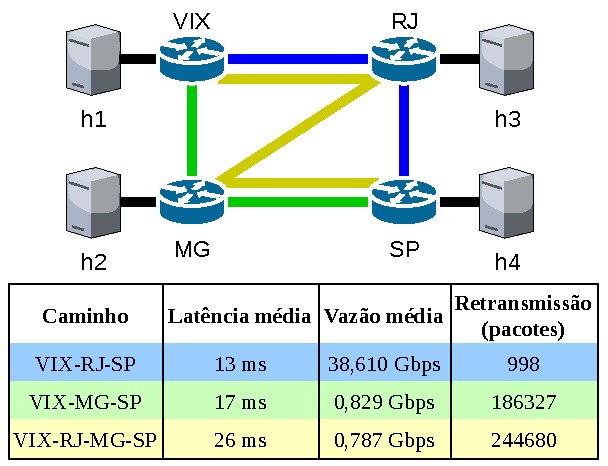
\includegraphics[width=0.65\linewidth]{figuras/Porvir - Tabela e Topo.pdf}
    \caption{Topologia interestadual do testbed nacional PORVIR utilizada no Protótipo 1.}
    \label{fig:porvir_topo}
\end{figure}

Nesse ambiente, o plano de controle é gerenciado pelo \textit{framework} freeRtr, responsável pela descoberta da topologia, pela atribuição dos identificadores polinomiais (\nodeIDs) a cada comutador de núcleo e pelo cálculo dos rótulos de roteamento na origem via Teorema Chinês dos Restos (CRT). Para possibilitar o isolamento de tráfego por meio da seleção explícita de caminhos fim a fim, foram provisionados três túneis PolKA distintos entre as bordas de Vitória e São Paulo:
\begin{itemize}
    \item \textbf{Caminho principal (VIX--RJ--SP):} rota de menor número de saltos e maior capacidade nominal, destinada às fatias de maior prioridade;
    \item \textbf{Caminho alternativo 1 (VIX--MG--SP):} rota intermediária utilizada para o desvio de fluxos concorrentes;
    \item \textbf{Caminho alternativo 2 (VIX--RJ--MG--SP):} rota secundária de maior comprimento, empregada para acomodar fluxos de menor precedência sob condições de competição no enlace principal.
\end{itemize}

A reconfiguração dinâmica das fatias nesse protótipo ocorre exclusivamente nos comutadores de borda, onde o plano de controle atualiza a associação entre o fluxo ingressante e o rótulo PolKA correspondente ao túnel de destino, redirecionando o tráfego sem alterar regras nos nós intermediários do núcleo.

% ==============================================================================
\section{Protótipo 2 -- SPolKA em Plano de Dados P4 (BMv2/Mininet)}
\label{sec:prototipo_bmv2}

Para validar o fatiamento conjunto de rotas explícitas e políticas de enfileiramento do \nome, desenvolveu-se o segundo protótipo no emulador de redes Mininet utilizando comutadores programáveis baseados na arquitetura comportamental BMv2 (\textit{Behavioral Model version 2}). A topologia experimental adotada, apresentada na Figura~\ref{fig:topologia_polka}, é composta por comutadores de borda (\texttt{e1} a \texttt{e6}), comutadores de núcleo (\texttt{s1} a \texttt{s4}, correspondentes aos nós $C_2$ a $C_5$ na representação lógica) e pares de \textit{hosts} geradores e receptores de tráfego ($H_1$--$S_1$ a $H_5$--$S_5$), interconectados por enlaces com capacidade configurada em 10~Mbps.

\begin{figure}[htbp]
    \centering
    \captionsetup{justification=centering}
    \fbox{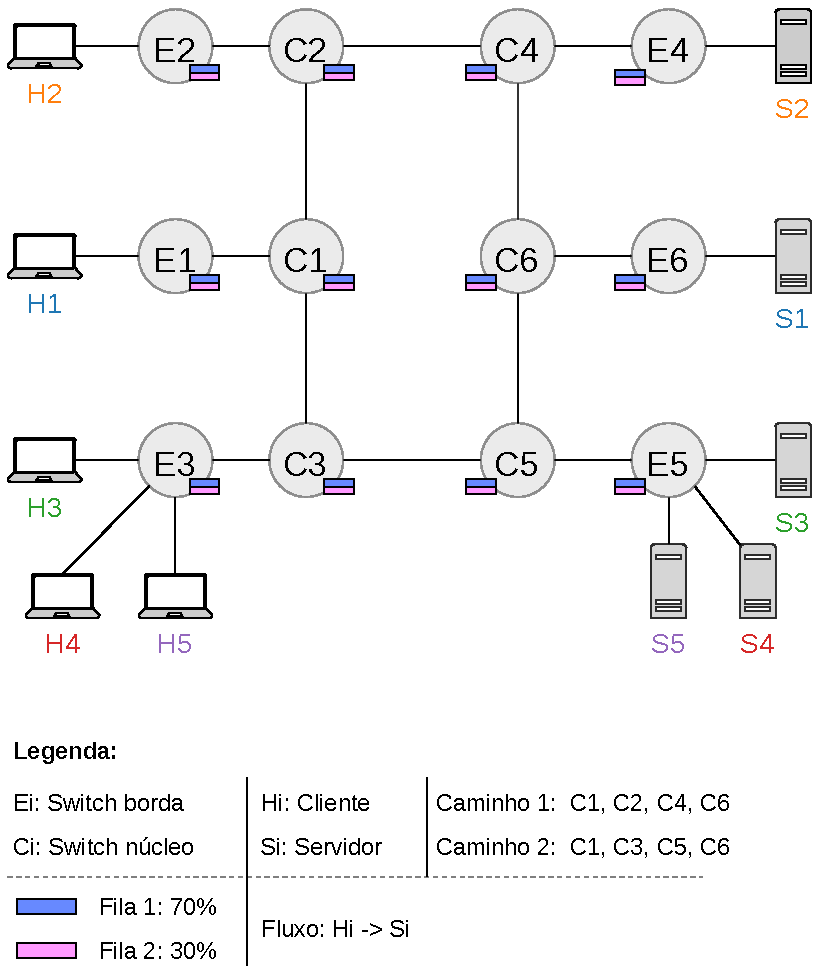
\includegraphics[width=0.75\linewidth]{figuras/topologia - SBRC WPEIF 2026_v4.pdf}}
    \caption{Topologia de rede emulada em Mininet/BMv2 para o Protótipo 2.}
    \label{fig:topologia_polka}
\end{figure}

Diferentemente do Protótipo 3 --- que classifica os pacotes com base no campo DSCP ---, no Protótipo 2 a identificação e o mapeamento das fatias na borda de ingresso são realizados a partir do **endereço IPv4 de origem** (\texttt{hdr.ipv4.srcAddr}) do fluxo entrante, demonstrando a flexibilidade do \nome\ em operar sobre distintos critérios de classificação do cabeçalho. A arquitetura interna do ambiente emulado divide-se em três componentes principais:

\begin{enumerate}
    \item \textbf{Plano de Controle e Síntese Polinomial:} 
    Um controlador centralizado implementado em Python calcula os rótulos \routeID\ de 160~bits (20~bytes, dimensionados para um diâmetro máximo de 10~saltos com polinômios geradores de grau 16) por meio da aplicação do Teorema Chinês dos Restos (CRT) polinomial sobre $GF(2)$. Em tempo de execução, o controlador povoa dinamicamente as tabelas de fluxo exclusivamente nos comutadores de borda, associando o endereço IPv4 de origem de cada fluxo ao respectivo \routeID\ codificado com a rota e a fila de serviço desejada.
    \item \textbf{Pipeline Programável em $\text{P4}_{16}$:} 
    Nos nós de borda, tabelas de correspondência exata sobre o endereço IPv4 de origem acionam a inserção do cabeçalho \nome\ (\textit{EtherType} \texttt{0x1234}) contendo o \routeID\ de 160~bits na entrada do domínio e sua remoção na borda de egresso antes da entrega ao \textit{host} de destino. Nos nós de núcleo, cada comutador executa a decodificação aritmética sem estado (\texttt{srcRoute\_nhop()}, Quadro~\ref{quad:codigo_controle}), empregando a primitiva de \textit{hash} CRC-16 customizado e o fatiamento de bits (\textit{bit-slicing}) para extrair simultaneamente a porta física de saída (\portID) e o identificador da fila (\qID).
    \item \textbf{Gerenciador de Tráfego (Traffic Manager) em C++:} 
    Como o escalonador nativo do BMv2 opera estritamente por prioridade fixa --- sujeitando filas de menor precedência à inanição (\textit{starvation}) ---, modificou-se o alvo \texttt{simple\_switch} do BMv2 para integrar um módulo externo (\textit{software extern}) em C++ baseado em \textcite{Elbediwy2025}, acoplado ao final do pipeline de \textit{Ingress}. O escalonador implementa o algoritmo \textit{Weighted Deficit Round-Robin} (WDRR) aliado a um buffer de pacotes (\texttt{TM\_buffer\_WDRR}) e a um conformador de taxa (\textit{token bucket shaper}) de 10~Mbps por interface.
\end{enumerate}

Para os testes de isolamento e migração de políticas de QoS conduzidos neste ambiente, cada interface de egresso dos roteadores de núcleo foi parametrizada com duas filas de serviço distintas no escalonador WDRR:
\begin{itemize}
    \item \textbf{Fila 1 (\texttt{qID = 001}):} fila prioritária com reserva garantida de \textbf{70\%} da largura de banda do enlace;
    \item \textbf{Fila 2 (\texttt{qID = 010}):} fila secundária com reserva garantida de \textbf{30\%} da largura de banda remanescente, capaz de aproveitar a capacidade ociosa da Fila 1 em períodos sem tráfego prioritário graças à natureza conservadora de trabalho (\textit{work-conserving}) do WDRR.
\end{itemize}
% ==============================================================================
\section{Protótipo 3 -- SPolKA em eBPF/XDP sobre Contêineres (Containerlab)}
\label{sec:prototipo_containerlab}

O terceiro protótipo foi concebido para validar a portabilidade e o desempenho do \nome\ diretamente no subsistema de rede do \textit{kernel} Linux em enlaces de 1~Gbps, sem dependência de simuladores comportamentais. A infraestrutura experimental é orquestrada via \textit{Containerlab} sobre 14 nós baseados em contêineres Ubuntu 24.04 LTS, seguindo a topologia apresentada na Figura~\ref{fig:topologia_ebpf}.

\begin{figure}[htbp]
    \centering
    \captionsetup{justification=centering}
    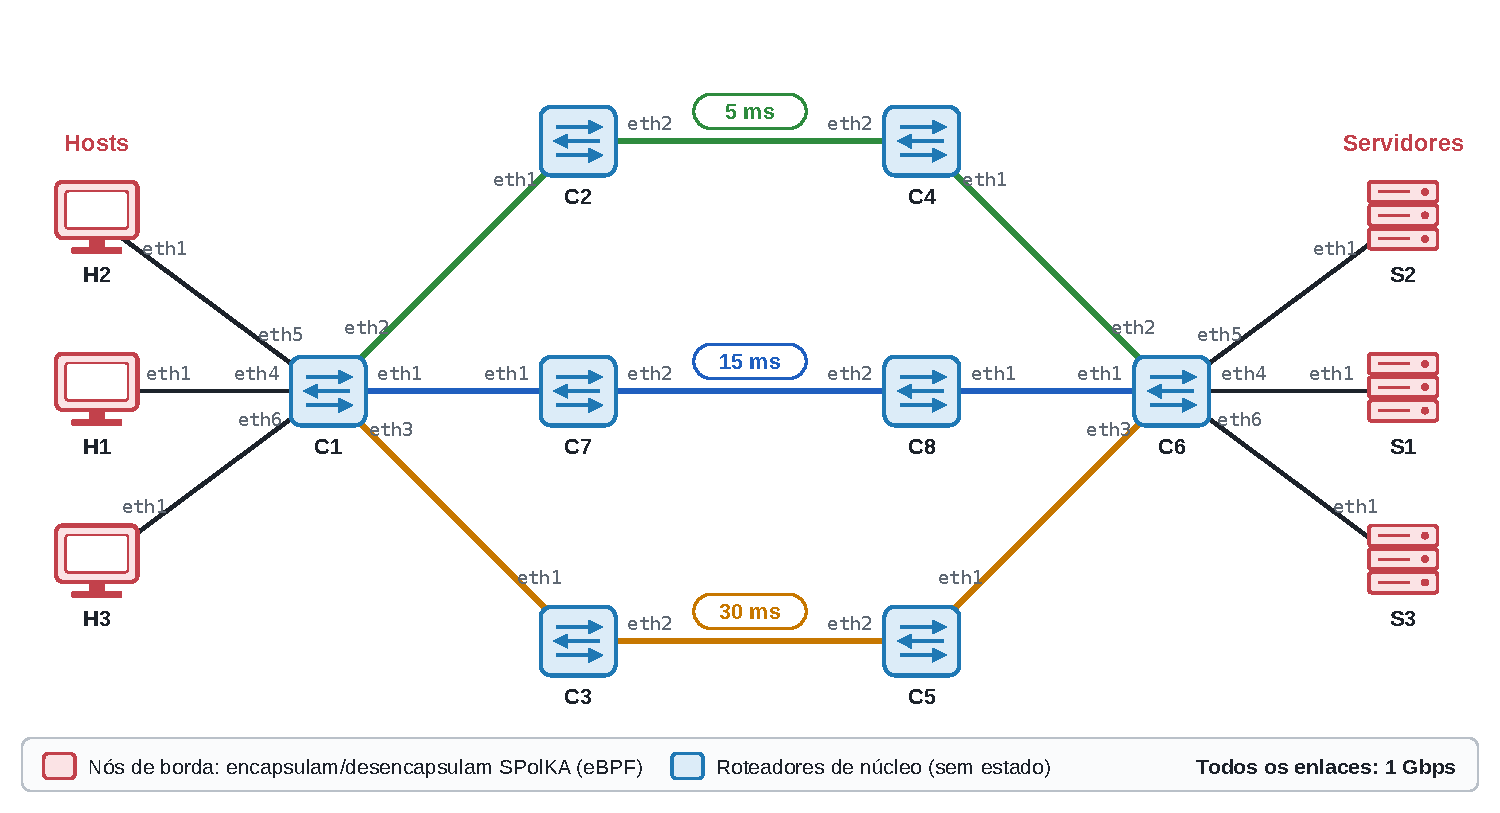
\includegraphics[width=0.85\linewidth]{figuras/fig_topologia_ebpf.pdf}
    \caption{Topologia de rede virtualizada em Containerlab/eBPF para o Protótipo 3.}
    \label{fig:topologia_ebpf}
\end{figure}

Conforme ilustrado na Figura~\ref{fig:topologia_ebpf}, a planta física interconecta três \textit{hosts} geradores ($H_1$, $H_2$ e $H_3$, na sub-rede \texttt{10.0.0.0/24}) e três servidores receptores ($S_1$, $S_2$ e $S_3$, na sub-rede \texttt{10.0.1.0/24}) via enlaces virtuais (\textit{veth}) de \textbf{1~Gbps}. Os próprios nós terminais ($H_1$--$H_3$ e $S_1$--$S_3$) atuam como \textbf{nós de borda} na interface \texttt{eth1}, enquanto os oito roteadores intermediários ($C_1$ a $C_8$) compõem o \textbf{núcleo sem estado} (\textit{stateless}), formando três caminhos disjuntos entre $C_1$ e $C_6$ com perfis distintos de latência de ida e volta (RTT):
\begin{itemize}
    \item \textbf{Caminho 1 ($C_1 \rightarrow C_2 \rightarrow C_4 \rightarrow C_6$):} rota de baixa latência com RTT configurado em \textbf{5~ms};
    \item \textbf{Caminho 2 ($C_1 \rightarrow C_7 \rightarrow C_8 \rightarrow C_6$):} rota de latência moderada com RTT configurado em \textbf{15~ms};
    \item \textbf{Caminho 3 ($C_1 \rightarrow C_3 \rightarrow C_5 \rightarrow C_6$):} rota de maior latência com RTT configurado em \textbf{30~ms}.
\end{itemize}

Para acomodar o cabeçalho compacto do \nome\ --- dimensionado neste protótipo em \textbf{8~bytes} (\textit{EtherType} \texttt{0x1234}) --- dentro do quadro Ethernet padrão de 1500~bytes sem fragmentação, as interfaces \texttt{eth1} das bordas são configuradas com MTU de 1492~bytes e ajuste automático de MSS TCP para 1420~bytes via \texttt{iptables}. Diferentemente do Protótipo 2, que requer um módulo externo em C++ no BMv2, o plano de dados em Linux divide-se em três programas eBPF compilados em C e fixados no sistema de arquivos BPF (\texttt{/sys/fs/bpf}):

\begin{enumerate}
    \item \textbf{Encapsulamento na Borda de Egresso (\texttt{spolka\_edge\_encap.c}, Apêndice~\ref{apendice:encap}):} Anexado ao gancho \texttt{TC egress} da interface \texttt{eth1} das bordas, intercepta pacotes IPv4 e realiza uma busca por correspondência de prefixo mais longo em um mapa LPM Trie (\texttt{BPF\_MAP\_TYPE\_LPM\_TRIE}, denominado \texttt{tabela\_encap}). A chave de busca combina o endereço IPv4 de destino (32~bits) e o campo DSCP mascarado (8~bits): entradas específicas de 40~bits associam uma classe de serviço a um \routeID\ dedicado, enquanto entradas de 32~bits atuam como rota padrão por destino. Identificado o fluxo, o programa insere os 8~bytes do cabeçalho \nome\ por meio da primitiva \texttt{bpf\_skb\_change\_head()}, preservando os metadados de checksum e segmentação (GSO) da pilha TCP/IP.
    \item \textbf{Encaminhamento e Classificação de Fila no Núcleo (\texttt{spolka\_core.c}, Apêndice~\ref{apendice:core}):} Anexado ao gancho \texttt{TC ingress} (\texttt{clsact}) de cada interface de dados (\texttt{eth1} a \texttt{eth6}) dos roteadores $C_1$ a $C_8$, aos quais são atribuídos polinômios irredutíveis únicos de grau 6 (\texttt{0x43} a \texttt{0x73}). Ao receber um quadro com \textit{EtherType} \texttt{0x1234}, o programa executa a divisão polinomial em $GF(2)$ diretamente em registradores de 32~bits (\texttt{poly\_mod}), extrai os 3~bits menos significativos referentes à fila (\texttt{queue\_id}) e os bits superiores referentes à porta lógica de saída (\texttt{logical\_port}), traduzindo-a para o índice de interface do \textit{kernel} via \texttt{mapa\_portas}. Em seguida, grava a fila selecionada nos metadados do pacote (\texttt{skb->priority = 0x00010000 | queue\_id}) e encaminha o quadro diretamente à fila de saída da porta de destino via \texttt{bpf\_redirect()}.
    \item \textbf{Desencapsulamento na Borda de Ingresso (\texttt{spolka\_edge\_decap.c}, Apêndice~\ref{apendice:decap}):} Anexado ao gancho \textbf{XDP nativo} (\textit{eXpress Data Path}) da interface \texttt{eth1} das bordas receptoras, remove os 8~bytes do rótulo \nome\ por meio da função \texttt{bpf\_xdp\_adjust\_head()}, restaura o \textit{EtherType} para IPv4 (\texttt{0x0800}) e entrega o pacote nativo à pilha de rede do contêiner (\texttt{XDP\_PASS}).
\end{enumerate}

Na saída de cada interface dos roteadores de núcleo, o escalonamento das fatias é realizado pelo subsistema nativo \textit{Traffic Control} (\texttt{tc}) do \textit{kernel} Linux. A hierarquia de enfileiramento combina uma disciplina \texttt{netem} na raiz (responsável por aplicar a latência de propagação de cada caminho), um conformador \texttt{tbf} (\textit{Token Bucket Filter}) configurado para a taxa nominal de 1~Gbps e uma disciplina escalonadora \texttt{drr} (\textit{Deficit Round-Robin}, \textit{handle} \texttt{1:}) composta por sete classes isoladas (\texttt{1:1} a \texttt{1:7}) com filas \texttt{bfifo} nas folhas. O metadado \texttt{skb->priority} gravado pelo programa \texttt{spolka\_core.c} endereça diretamente a classe \texttt{1:N} correspondente sem necessidade de filtros adicionais no \texttt{tc}.

Para representar um cenário realista de fatiamento multiserviço em redes cientes de caminho, o protótipo foi parametrizado com sete classes de tráfego mapeadas via DSCP (Tabela~\ref{tab:classes_servico}) e sete filas DRR com \textit{quanta} dimensionados proporcionalmente às reservas de largura de banda sobre um MTU de 1500~bytes (Tabela~\ref{tab:filas_classe_servico}).

\begin{table}[htbp]
    \centering
    \caption{Especificação e parâmetros das classes de serviço configuradas no Protótipo 3.}
    \label{tab:classes_servico}
    \begin{tabularx}{\textwidth}{lcXccc}
        \toprule
        \textbf{Classe de Serviço} & \textbf{DSCP} & \textbf{Perfil de Tráfego} & \textbf{Taxa} & \textbf{Pacote (B)} & \textbf{Prot.} \\
        \midrule
        0: \textit{low\_latency}        & 46 (EF)   & Baixa latência     & 2,00 Mbit/s & 100  & UDP \\
        1: \textit{critical\_signaling} & 40 (CS5)  & Sinalização crítica & 0,30 Mbit/s & 250  & UDP \\
        2: \textit{high\_throughput}    & 26 (AF31) & Alta vazão         & Best-effort & 1500 & TCP \\
        3: \textit{long\_living}        & 18 (AF21) & Fluxo persistente  & Best-effort & 1500 & TCP \\
        4: \textit{short\_living}       & 10 (AF11) & Rajadas curtas     & Sondagem    & 100  & ICMP \\
        5: \textit{intent\_based}       & 12 (AF12) & Baseado em intenção & 2,00 Mbit/s & 80   & UDP \\
        6: \textit{best\_effort}        & 0 (BE)    & Melhor esforço     & Best-effort & 1500 & TCP \\
        \bottomrule
    \end{tabularx}
    \fonte{Elaborado pelo autor (2026), adaptado de \textcite{puttaswamy2025pathaware}.}
\end{table}

\begin{table}[htbp]
    \centering
    \caption{Parâmetros de configuração, reserva de vazão e \textit{quantum} DRR das filas no Linux \texttt{tc}.}
    \label{tab:filas_classe_servico}
    \begin{tabularx}{\textwidth}{cccX}
        \toprule
        \textbf{Fila (\texttt{qID})} & \textbf{Banda (\%)} & \textbf{Quantum DRR (B)} & \textbf{Classe de Serviço Associada} \\
        \midrule
        1 (\texttt{1:1}) & 5  & 3.750  & \textit{Low Latency Class} \\
        2 (\texttt{1:2}) & 5  & 3.750  & \textit{Critical Signaling / Priority Class} \\
        3 (\texttt{1:3}) & 60 & 45.000 & \textit{High Throughput Class} \\
        4 (\texttt{1:4}) & 20 & 15.000 & \textit{Long Living Class} \\
        5 (\texttt{1:5}) & 3  & 2.250  & \textit{Short Living Class} \\
        6 (\texttt{1:6}) & 5  & 3.750  & \textit{Intent Based Class} \\
        7 (\texttt{1:7}) & 2  & 1.500  & \textit{Best Effort / Default Flow Class} \\
        \bottomrule
    \end{tabularx}
    \fonte{Elaborado pelo autor (2026).}
\end{table}

Com as infraestruturas experimentais, os planos de dados e os parâmetros de enfileiramento dos três protótipos devidamente especificados, o Capítulo~\ref{chap:avaliacao} apresenta a metodologia de testes, os cenários de carga avaliados e a análise comparativa dos resultados obtidos.f
% ---
% ------------------------ AVALIAÇÃO E RESULTADOS ------------------
% ---

\chapter{AVALIAÇÃO E RESULTADOS}
\label{chap:avaliacao}

Este capítulo apresenta a avaliação experimental e a análise dos resultados obtidos nos três protótipos desenvolvidos para validar a arquitetura \nome\ e compará-la ao protocolo \polka\ original. Seguindo a estratégia incremental detalhada no Capítulo~\ref{chap:prototipos}, os ensaios exploram desde a seleção explícita de caminhos em hardware programável de alta capacidade até o fatiamento conjunto de rotas e políticas de enfileiramento em planos de dados emulados em P4 e acelerados via eBPF/XDP no \textit{kernel} Linux.

% ==============================================================================
\section{Metodologia Experimental e Métricas Avaliadas}
\label{sec:metodologia_avaliacao}

Para avaliar de forma abrangente a eficácia do isolamento de recursos, a previsibilidade de atraso e a agilidade na reconfiguração dinâmica das fatias de rede sem manutenção de estados no núcleo, os experimentos foram organizados em três frentes complementares:

\begin{itemize}
    \item \textbf{Protótipo 1 (\textit{Testbed} PORVIR -- Hardware Intel Tofino/freeRtr):} avalia o fatiamento baseado exclusivamente na seleção explícita de caminhos fim a fim no \polka\ original sobre enlaces físicos interestaduais de 10~Gbit/s;
    \item \textbf{Protótipo 2 (Emulação P4/BMv2 com \textit{Traffic Manager} WDRR):} valida o encapsulamento unificado de rota e fila (\routeID) do \nome\ em enlaces de 10~Mbit/s, verificando o isolamento ponderado de banda e a migração dinâmica de políticas em duas rodadas experimentais;
    \item \textbf{Protótipo 3 (Virtualização Containerlab com eBPF/XDP e Linux \texttt{tc}):} investiga o comportamento do \nome\ em enlaces de 1~Gbit/s sob cargas heterogêneas multiserviço (fluxos UDP sensíveis a atraso e fluxos TCP elásticos), comparando progressivamente os escalonadores FIFO, WDRR e SP-WDRR, bem como os algoritmos de controle de congestionamento CUBIC e BBR.
\end{itemize}

Na geração de cargas de trabalho e instrumentação das medições, empregou-se a ferramenta \texttt{iperf3} para injeção de fluxos TCP e UDP e aferição de vazão efetiva, \textit{jitter} (conforme RFC~3550), taxa de perda e volume de retransmissões TCP, além de sondas ICMP (\texttt{ping}) para monitoramento contínuo do tempo de ida e volta (RTT) médio, máximo e de cauda (95º percentil). Nos ensaios do Protótipo~3, também foram coletadas estatísticas internas diretamente das disciplinas de enfileiramento do subsistema \texttt{tc} do \textit{kernel} Linux (ocupação de \textit{buffer}/\textit{backlog} e contagem de pacotes por fila salto a salto).

% ==============================================================================
\section{Protótipo 1 -- PolKA Original em Hardware Programável}
\label{sec:res_prototipo1}

O primeiro protótipo foi avaliado no \textit{testbed} nacional PORVIR~\cite{Nogueira2025}, composto por quatro nós implementados em comutadores programáveis Intel Tofino\textregistered\ gerenciados pelo plano de controle \texttt{freeRtr}\footnote{\url{http://www.freertr.org/}} (topologia ilustrada na Figura~\ref{fig:porvir_topo}). Para avaliar individualmente o desempenho das rotas disponíveis entre Vitória e São Paulo, foram provisionados três túneis \polka\ distintos: \texttt{VIX--RJ--SP}, \texttt{VIX--MG--SP} e \texttt{VIX--RJ--MG--SP}.

\subsection{Caracterização de Desempenho dos Caminhos}
\label{subsec:porvir_caracterizacao}

Inicialmente, caracterizou-se o desempenho basal de cada rota em termos de latência média, vazão média e volume de retransmissões, conforme sintetizado na Tabela~\ref{tab:metricas_porvir}. As medições de tráfego TCP foram conduzidas via \texttt{iperf3} durante 60 minutos para cada caminho, com amostragens coletadas a cada 30 segundos, enquanto o RTT médio foi aferido por meio de sondas ICMP (\texttt{ping}) em intervalos de 1 segundo ao longo do mesmo período.

\begin{table}[htbp]
\centering
\caption{Métricas de desempenho por caminho no \textit{testbed} PORVIR (Protótipo 1).}
\label{tab:metricas_porvir}
\begin{tabularx}{\textwidth}{Xccc}
\toprule
\textbf{Caminho} & \textbf{Latência média} & \textbf{Vazão média} & \textbf{Retransmissões (pacotes)} \\
\midrule
\texttt{VIX--RJ--SP}     & 13~ms & 38,610~Gbit/s & 998 \\
\texttt{VIX--MG--SP}     & 17~ms & 0,829~Gbit/s  & 186.327 \\
\texttt{VIX--RJ--MG--SP} & 26~ms & 0,787~Gbit/s  & 244.680 \\
\bottomrule
\end{tabularx}
\fonte{Elaborado pelo autor (2026).}
\end{table}

Os resultados evidenciam que o caminho principal \texttt{VIX--RJ--SP} apresenta desempenho substancialmente superior aos demais, registrando vazão média aproximadamente 46 vezes maior (38,610~Gbit/s), menor atraso médio (13~ms) e número reduzido de retransmissões (998 pacotes), ao passo que \texttt{VIX--MG--SP} e \texttt{VIX--RJ--MG--SP} atuam como rotas alternativas de menor capacidade.

\subsection{Isolamento e Migração Dinâmica de Fatias}
\label{subsec:porvir_migracao}

Após a etapa de caracterização, executou-se um experimento com três fluxos TCP concorrentes gerados via \texttt{iperf3} sobre o enlace de alta capacidade (\texttt{VIX--RJ--SP}), representando a coexistência entre uma fatia de rede prioritária (Fluxo~1) e duas fatias de menor prioridade (Fluxos~2 e~3). Nesse cenário, cada fluxo opera como uma fatia independente, recebendo recursos isolados e sendo reconfigurado dinamicamente na borda conforme seus requisitos de QoS.

\begin{figure}[htbp]
    \centering
    \captionsetup{justification=centering}
    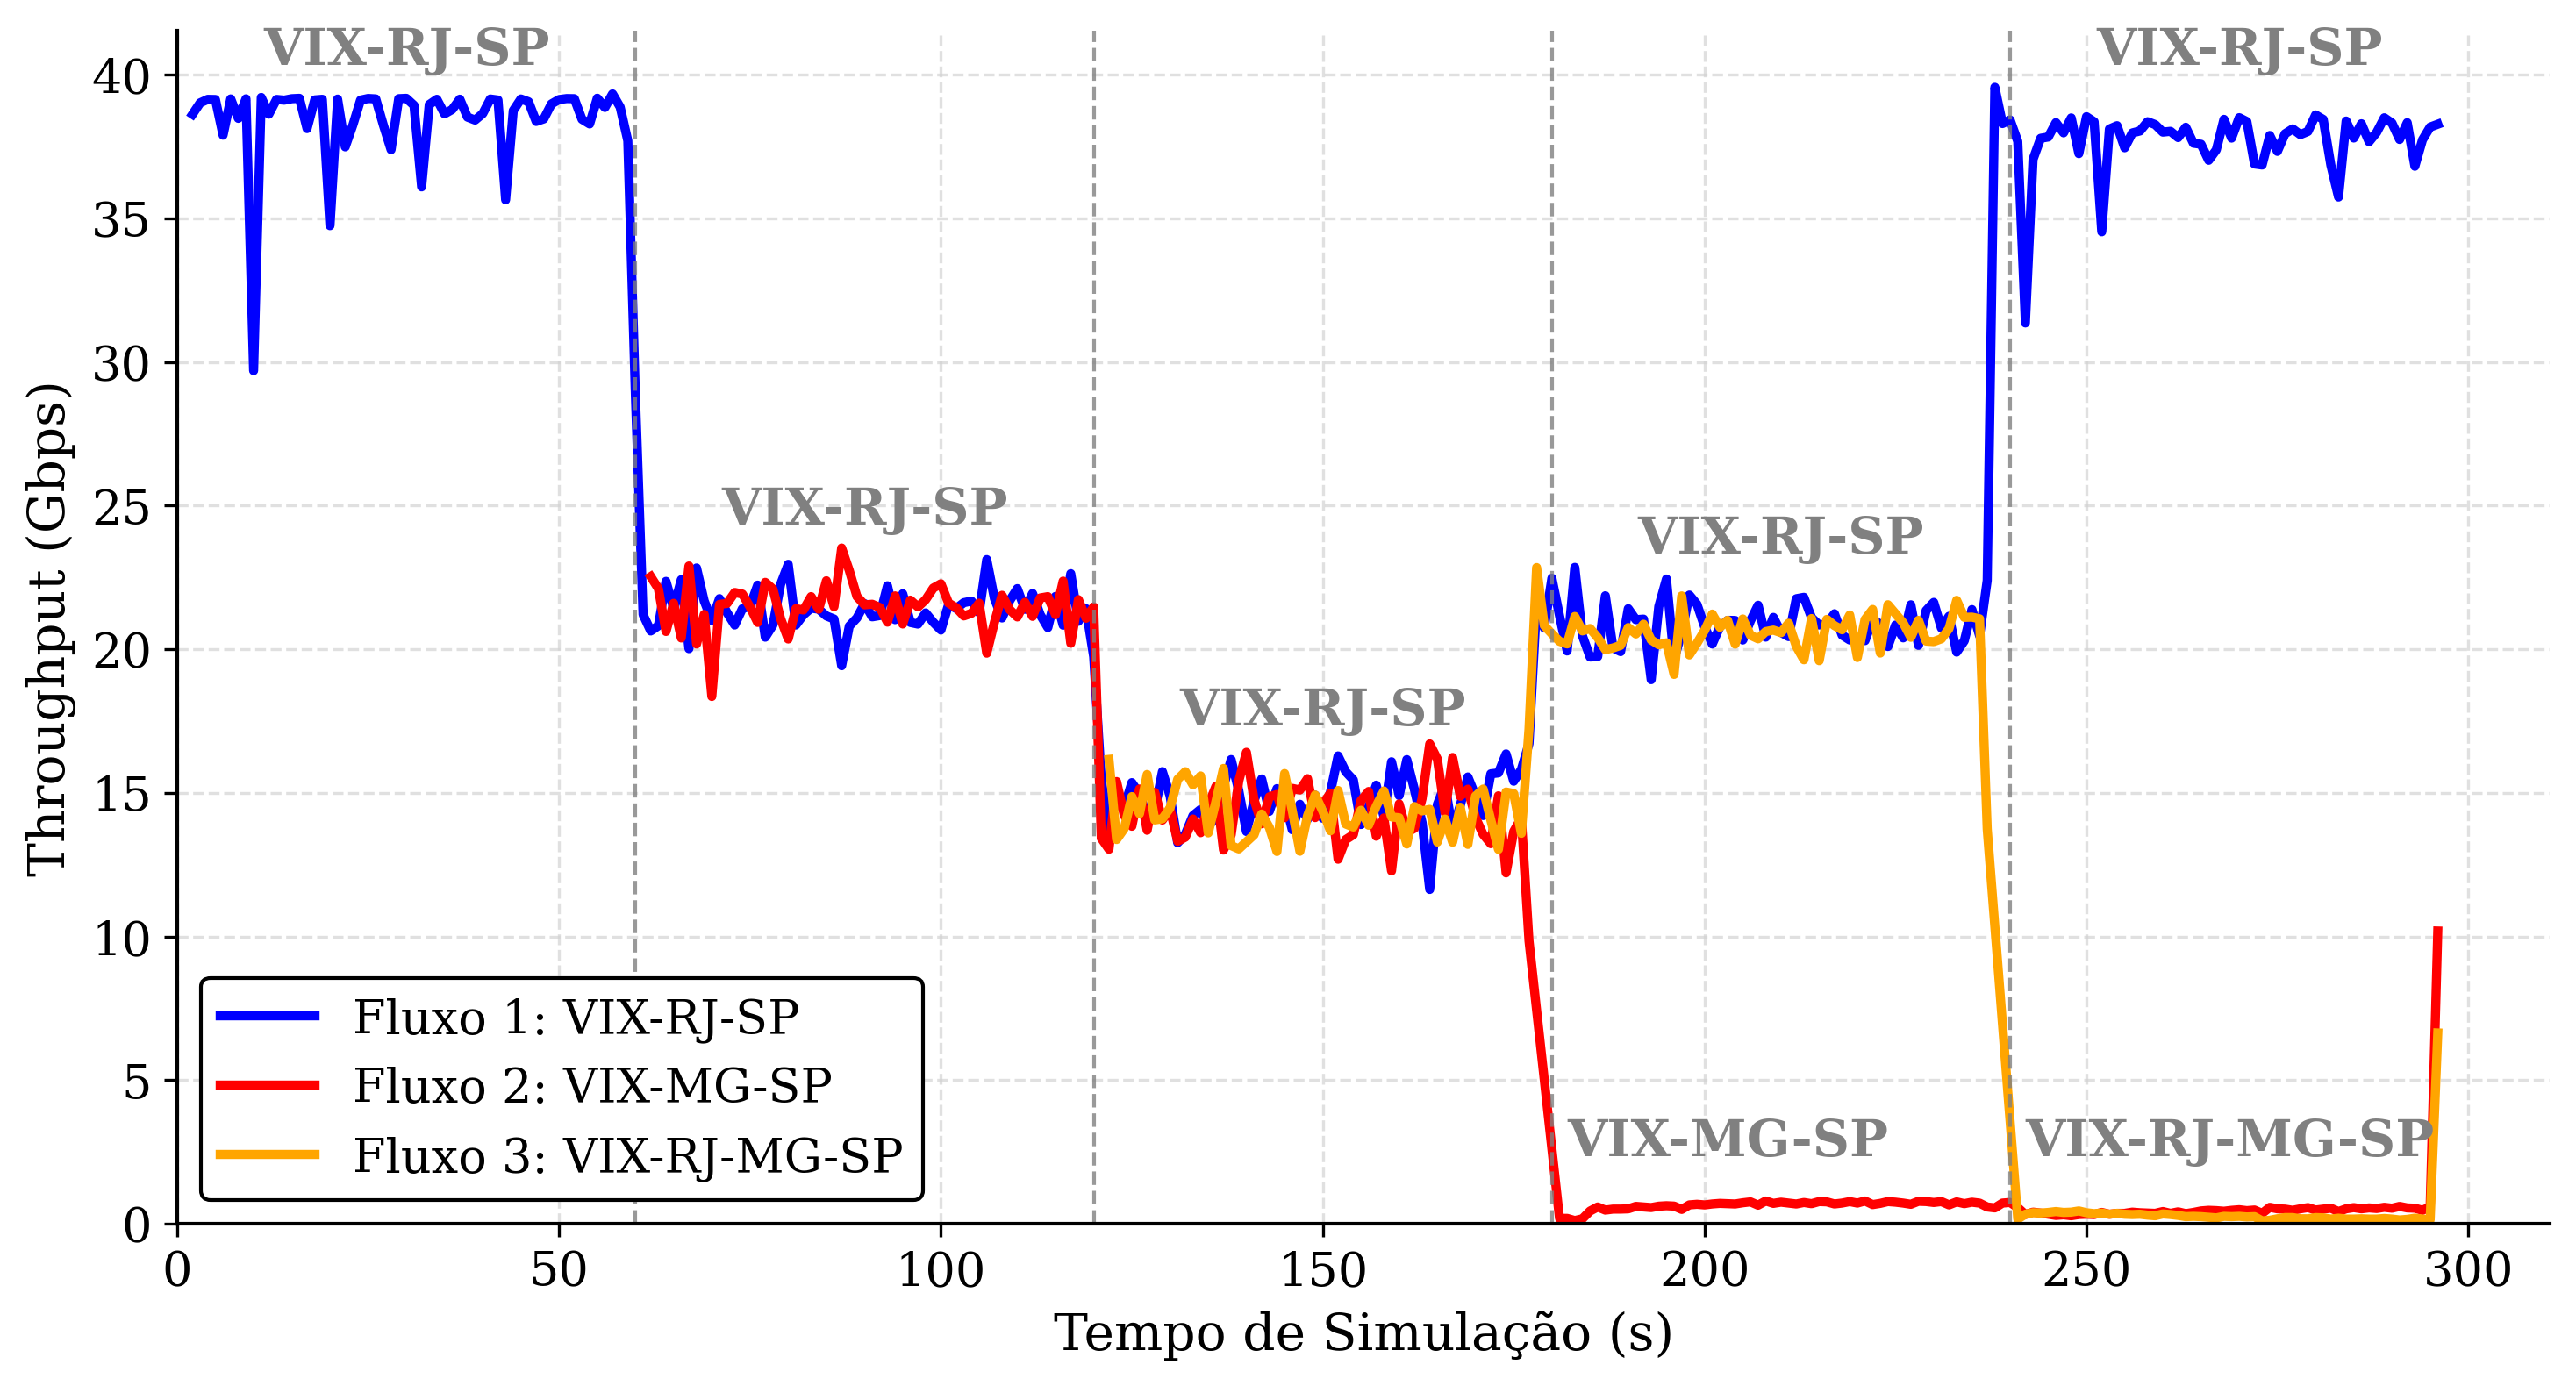
\includegraphics[width=0.85\linewidth]{figuras/grafico_mudanca_caminho_porvir.png}
    \caption{Evolução temporal da vazão e migração dinâmica de caminhos no \textit{testbed} PORVIR (Protótipo 1).}
    \label{fig:porvir_vazao}
\end{figure}

A Figura~\ref{fig:porvir_vazao} apresenta a evolução temporal da vazão coletada ao longo dos eventos, espaçados em intervalos de 60 segundos e divididos em duas fases principais:

\begin{itemize}
    \item \textbf{Fase de competição ($0 \le t < 180\text{~s}$):} a fatia correspondente ao Fluxo~1 inicia operando isoladamente no caminho principal (\texttt{VIX--RJ--SP}), alcançando cerca de 38,6~Gbit/s. Nos instantes $t = 60\text{~s}$ e $t = 120\text{~s}$, as fatias concorrentes dos Fluxos~2 e~3 são ativadas sobre a mesma rota, passando a disputar a largura de banda do enlace e reduzindo a taxa efetiva de cada fluxo para aproximadamente 21~Gbit/s (com dois fluxos) e 14~Gbit/s (com três fluxos).
    \item \textbf{Fase de migração ($180 \le t \le 300\text{~s}$):} demonstrando o isolamento lógico e a adaptação dinâmica proporcionados pelo roteamento na origem, as fatias concorrentes são realocadas para rotas alternativas de menor capacidade sem necessidade de reconfiguração nos comutadores intermediários. O Fluxo~2 é migrado para o caminho \texttt{VIX--MG--SP} em $t = 180\text{~s}$, enquanto o Fluxo~3 é redirecionado para \texttt{VIX--RJ--MG--SP} em $t = 240\text{~s}$. Como resultado, a fatia prioritária do Fluxo~1 restabelece integralmente o uso da capacidade do enlace principal.
\end{itemize}

Apesar da eficácia demonstrada na seleção de rotas, o \polka\ original atua estritamente no nível de caminho, não oferecendo diferenciação por filas dentro de um mesmo enlace compartilhado --- limitação superada pela arquitetura \nome\ avaliada nos protótipos subsequentes.

% ==============================================================================
\section{Protótipo 2 -- SPolKA em Plano de Dados P4/BMv2}
\label{sec:res_prototipo2}

O segundo protótipo valida a arquitetura \nome\ em ambiente emulado (Mininet/BMv2) sobre a topologia da Figura~\ref{fig:topologia_polka}, na qual o identificador \routeID\ codifica simultaneamente a trajetória e a fila de escalonamento em cada salto. Conforme detalhado na Seção~\ref{sec:prototipo_bmv2}, cada interface de egresso dos roteadores de núcleo opera com enlaces de 10~Mbit/s e duas filas gerenciadas pelo \textit{Traffic Manager} customizado com algoritmo WDRR~\cite{Elbediwy2025}: a \textbf{Fila~1} (prioritária, com reserva de 70\% da banda) e a \textbf{Fila~2} (secundária, com reserva de 30\% da banda). Os fluxos de dados entre clientes ($H_i$) e servidores ($S_i$) foram gerados via \texttt{iperf3} utilizando o protocolo TCP em duas rodadas experimentais.

\subsection{Primeira Rodada -- Reconfiguração Dinâmica de Políticas de Filas}
\label{subsec:prot2_rodada1}

Na primeira rodada experimental, investigou-se exclusivamente o impacto da alteração dinâmica de filas sobre um mesmo caminho físico (\texttt{\{C1, C3, C5, C6\}}). Foram instanciadas três fatias de rede: uma fatia de alta prioridade, representada pelo fluxo $H_3 \rightarrow S_3$, e duas fatias de menor prioridade, representadas pelos fluxos $H_4 \rightarrow S_4$ e $H_5 \rightarrow S_5$, visando validar o isolamento de recursos em condições de saturação do enlace.

\begin{figure}[htbp]
    \centering
    \captionsetup{justification=centering}
    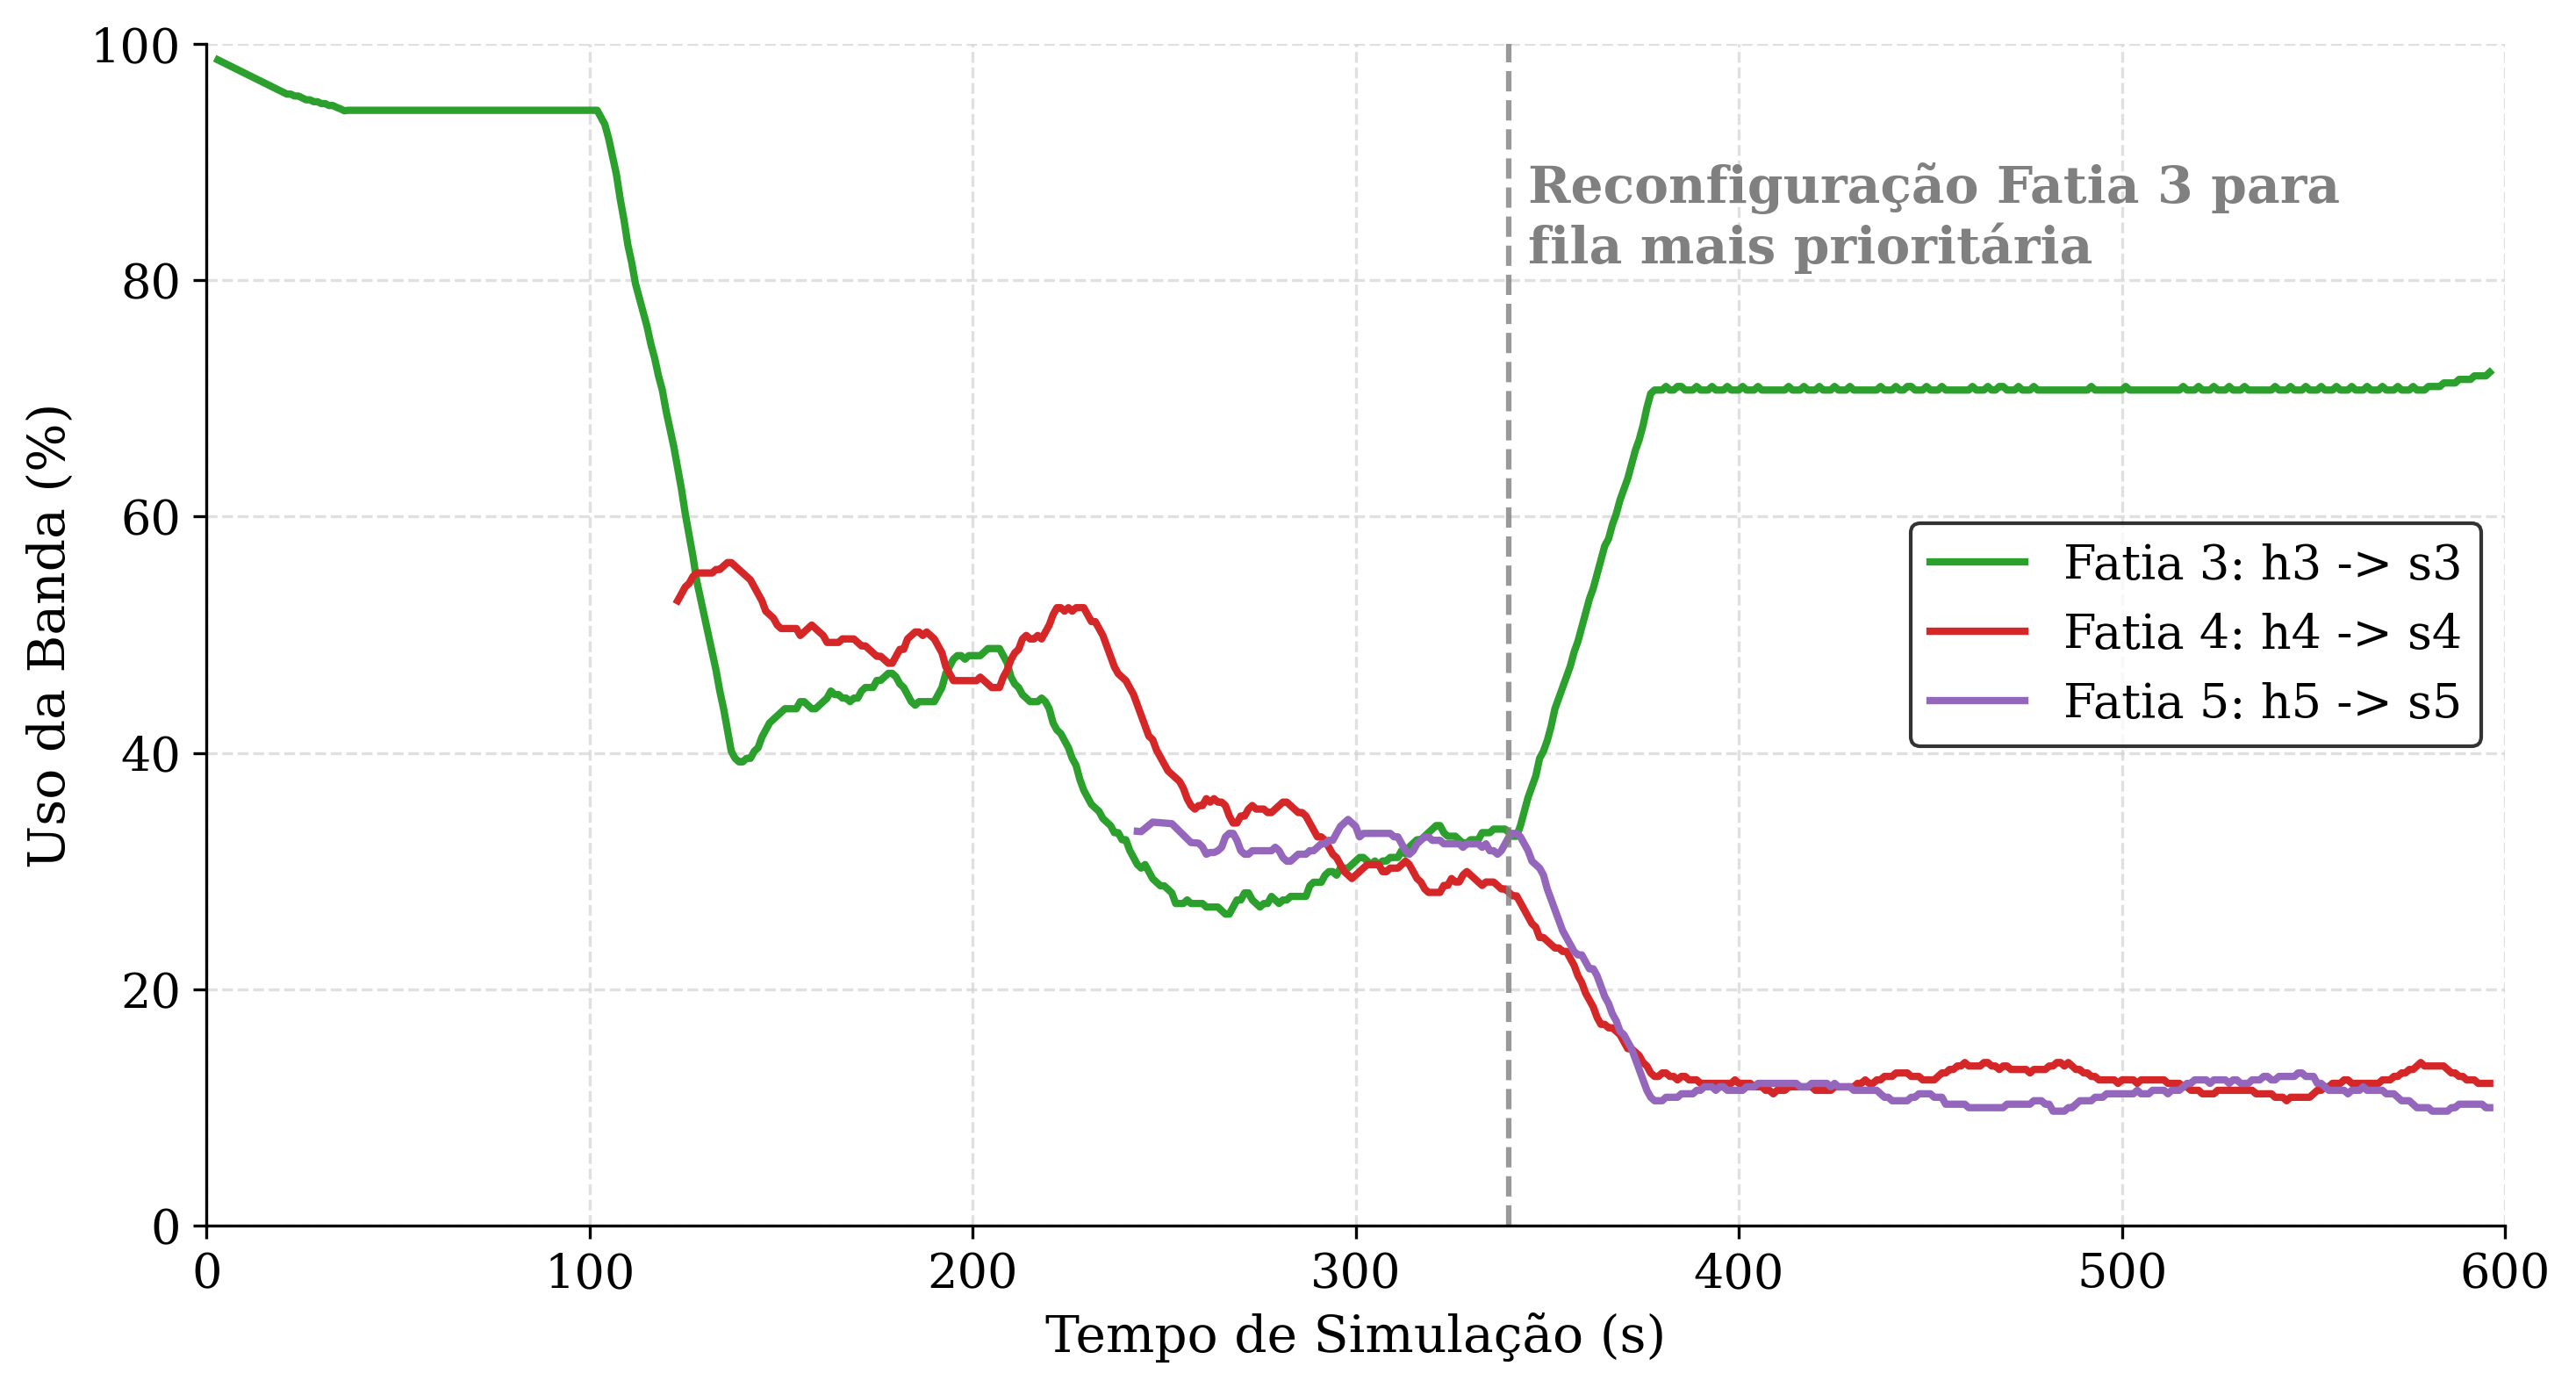
\includegraphics[width=0.85\linewidth]{figuras/grafico_mudanca_fila_polka.png}
    \caption{Ocupação de banda na primeira rodada do Protótipo 2: reconfiguração dinâmica da Fatia 3 para a fila prioritária.}
    \label{fig:mininet_mudanca_fila_polka}
\end{figure}

Conforme ilustrado na Figura~\ref{fig:mininet_mudanca_fila_polka}, o ensaio desenvolve-se em duas etapas principais:
\begin{itemize}
    \item \textbf{Compartilhamento inicial na fila secundária:} no início da execução, o fluxo $H_3 \rightarrow S_3$ (Fatia~3) é alocado na \textbf{Fila~2} em todos os saltos. Pela propriedade de conservação de trabalho (\textit{work-conserving}) do algoritmo WDRR, na ausência de tráfego na fila prioritária, a largura de banda total disponível no enlace é usufruída pela Fila~2. Com a entrada sequencial dos fluxos concorrentes $H_4 \rightarrow S_4$ (Fatia~4) e $H_5 \rightarrow S_5$ (Fatia~5) na mesma fila, a capacidade do enlace passa a ser dividida de forma equitativa entre as três fatias (cerca de 33\% para cada fluxo).
    \item \textbf{Promoção para a fila prioritária:} no instante de reconfiguração (destacado pela linha tracejada na Figura~\ref{fig:mininet_mudanca_fila_polka}), o comutador de borda atualiza o \routeID\ do fluxo $H_3 \rightarrow S_3$ para direcioná-lo à \textbf{Fila~1} (detentora de reserva estrita de 70\% da largura de banda). Essa alteração assegura imediatamente o isolamento de desempenho para a fatia prioritária, que estabiliza sua ocupação em 70\% da capacidade do enlace, enquanto os fluxos remanescentes na Fila~2 ($H_4$ e $H_5$) passam a competir estritamente pelos 30\% residuais.
\end{itemize}

\subsection{Segunda Rodada -- Migração Concomitante de Rotas e Filas}
\label{subsec:prot2_rodada2}

Na segunda rodada experimental, avaliou-se a capacidade do \nome\ de executar reconfigurações simultâneas de caminho e classe de serviço diante de congestionamentos localizados entre os dois caminhos da topologia: o Caminho~1 (\texttt{\{C1, C2, C4, C6\}}) e o Caminho~2 (\texttt{\{C1, C3, C5, C6\}}).

\begin{figure}[htbp]
    \centering
    \captionsetup{justification=centering}
    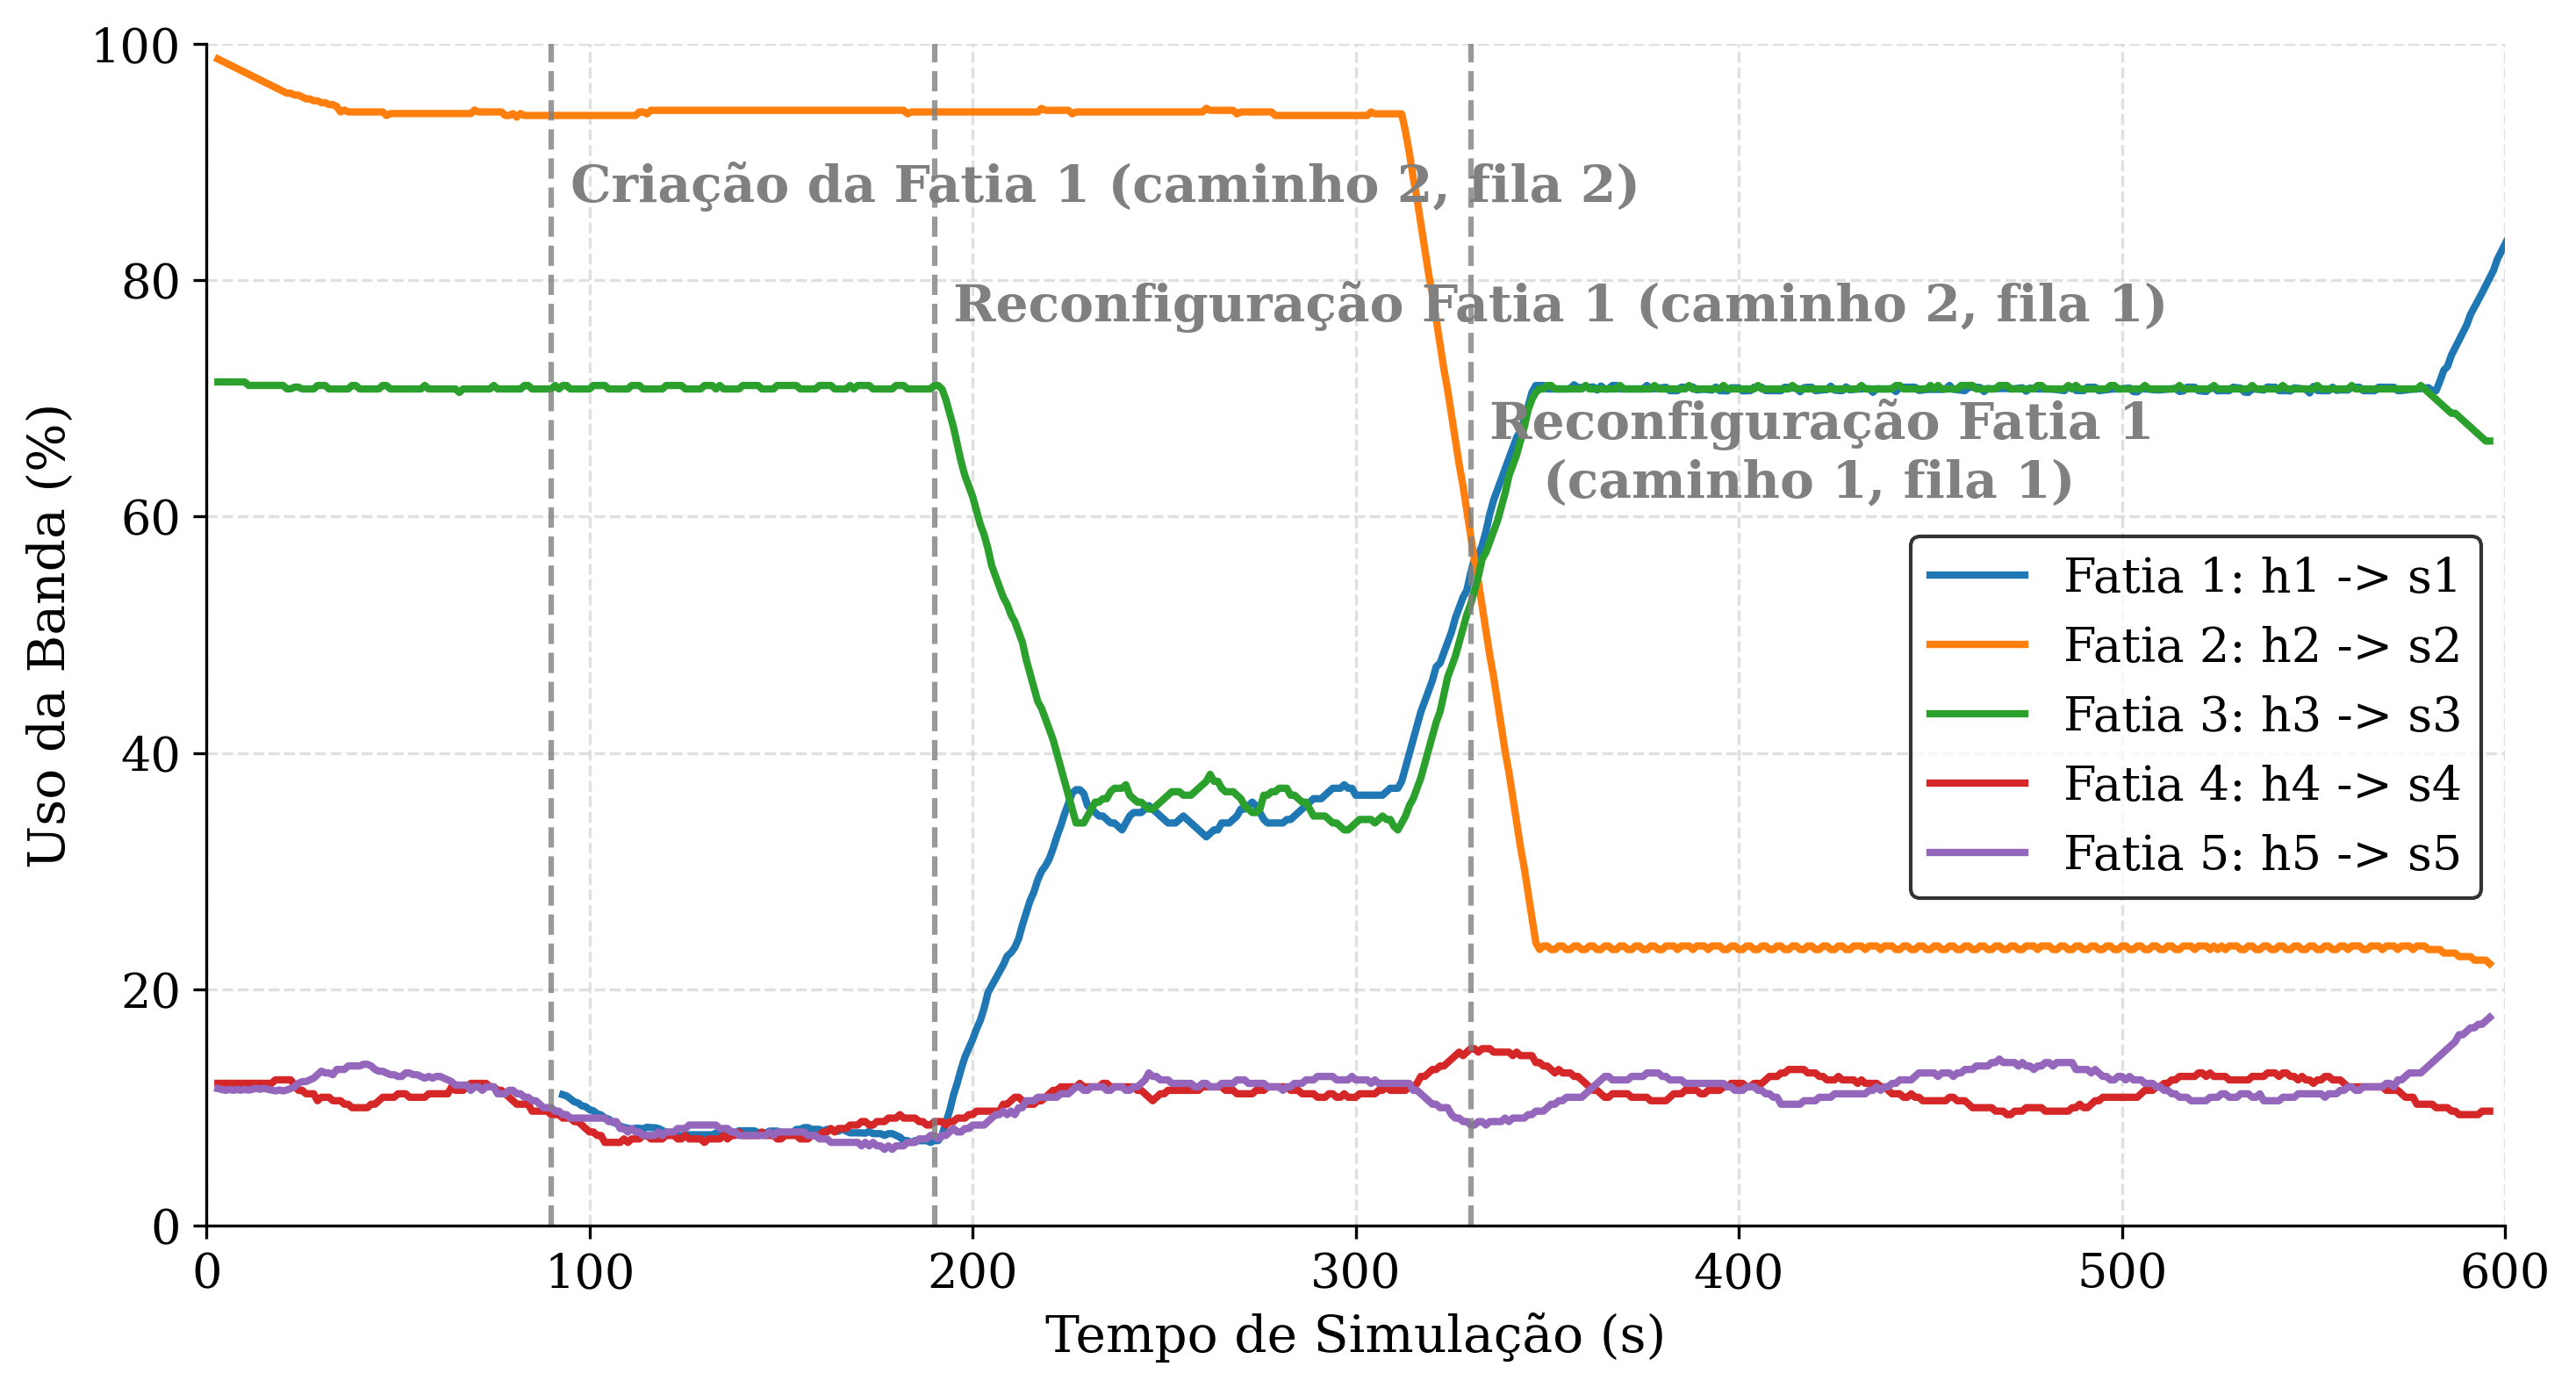
\includegraphics[width=0.85\linewidth]{figuras/grafico_mudanca_caminho_fila_polka.png}
    \caption{Ocupação de banda na segunda rodada do Protótipo 2: reconfiguração concomitante de fila e caminho para a Fatia 1.}
    \label{fig:mininet_mudanca_caminho_fila}
\end{figure}

A dinâmica observada na Figura~\ref{fig:mininet_mudanca_caminho_fila} divide-se em três fases operacionais:
\begin{itemize}
    \item \textbf{Estado inicial e inserção de carga concorrente:} inicialmente, instancia-se a fatia $H_2 \rightarrow S_2$ (Fatia~2) pelo Caminho~1 na Fila~2 --- ocupando praticamente toda a banda disponível (acima de 90\%) devido à ausência de tráfego concorrente naquela rota --- e três fatias pelo Caminho~2: $H_3 \rightarrow S_3$ (Fatia~3) na Fila~1 (70\% de reserva) e os fluxos $H_4 \rightarrow S_4$ e $H_5 \rightarrow S_5$ na Fila~2 (dividindo os 30\% restantes). Em seguida, introduz-se o fluxo $H_1 \rightarrow S_1$ (Fatia~1) pelo Caminho~2 na Fila~2, passando a competir pela reserva de 30\% com $H_4$ e $H_5$.
    \item \textbf{Elevação de prioridade na mesma rota:} na segunda etapa, o nó de borda reconfigura o rótulo da Fatia~1 ($H_1 \rightarrow S_1$) para promovê-la à Fila~1 mantendo o mesmo trajeto (Caminho~2). Como consequência, a Fatia~1 passa a compartilhar equitativamente a reserva de 70\% da Fila~1 com a Fatia~3 ($H_3 \rightarrow S_3$), registrando cerca de 35\% da banda para cada fluxo prioritário.
    \item \textbf{Migração de rota com manutenção de fila prioritária:} por fim, o nó de ingresso altera o \routeID\ da Fatia~1 para desviá-la ao Caminho~1 (\texttt{\{C1, C2, C4, C6\}}), preservando sua atribuição à Fila~1. Essa migração elimina a disputa por recursos críticos sem qualquer intervenção nos nós de núcleo: no Caminho~1, a Fatia~1 passa a usufruir isoladamente dos 70\% de banda da Fila~1, enquanto a Fatia~2 acomoda-se na reserva de 30\% da Fila~2; simultaneamente, no Caminho~2, a Fatia~3 recupera integralmente sua cota de 70\% na Fila~1.
\end{itemize}

% ==============================================================================
\section{Protótipo 3 -- SPolKA em eBPF/XDP sobre Contêineres}
\label{sec:res_prototipo3}

O terceiro protótipo avalia o desempenho do \nome\ diretamente no subsistema de rede do \textit{kernel} Linux (ambiente Containerlab, Figura~\ref{fig:topologia_ebpf}) em enlaces de 1~Gbit/s. Os ensaios submetem o caminho de menor latência ($C_1 \rightarrow C_2 \rightarrow C_4 \rightarrow C_6$, com RTT base de 5~ms) ao envio simultâneo de cinco fluxos concorrentes durante 300 segundos, contemplando duas classes UDP com taxa controlada (Classe~0: \textit{low\_latency} a 2,0~Mbit/s; Classe~1: \textit{critical\_signaling} a 0,3~Mbit/s) e três classes TCP elásticas (\textit{high\_throughput}, \textit{long\_living} e \textit{best\_effort}) parametrizadas conforme as Tabelas~\ref{tab:classes_servico} e~\ref{tab:filas_classe_servico}.

\subsection{Experimento 1 -- Tráfego sem Classificação de Prioridade (FIFO)}
\label{subsec:exp1_fifo}

Nesta primeira rodada de testes, avalia-se o comportamento base da rede operando sob uma disciplina de enfileiramento única do tipo \textit{First-In, First-Out} (FIFO), sem diferenciação ou isolamento entre as classes de serviço.

Os fluxos do protocolo UDP (classes 0 e 1) preservaram integralmente as vazões injetadas, registrando 2,0~Mbit/s e 0,3~Mbit/s com perdas irrelevantes de 0,006\% e 0,002\%, respectivamente. Tal comportamento deve-se à natureza dessas fontes em malha aberta --- desprovidas de controle de congestionamento para desaceleração --- e ao fato de sua carga combinada (2,3~Mbit/s) corresponder a apenas 0,23\% da capacidade do enlace. Contudo, a manutenção da vazão não impediu a degradação da latência: o RTT dessas classes saltou do tempo de propagação base de 5~ms para uma média de 10,49~ms, atingindo picos de 27,9~ms devido ao atraso gerado pelo compartilhamento da fila com o tráfego TCP. Assim, no regime FIFO, a garantia da vazão da classe de baixa latência ocorre à custa de um aumento substancial no atraso.

Por outro lado, as três correntes TCP, reguladas pelo mecanismo de controle de congestionamento CUBIC, responderam às perdas de pacotes (que somaram 19.300 retransmissões) ajustando suas janelas de congestionamento e dividindo de forma equilibrada a capacidade excedente do enlace: 302,2~Mbit/s, 292,5~Mbit/s e 297,9~Mbit/s (Figura~\ref{fig:exp1_fifo}, painel (a)). Isso representa uma variação inferior a 3\% na média do ensaio, embora seus perfis de vazão instantânea tenham apresentado flutuações e alternâncias no decorrer dos 300 segundos de execução. Cabe destacar que, apesar de pertencerem a categorias nominalmente distintas (\texttt{high\_throughput}, \texttt{long\_living} e \texttt{best\_effort}) e estarem associadas a filas separadas nas configurações, a ausência de uma política de escalonamento por classe invalida esses mapeamentos, impondo um tratamento uniforme a todas elas.

\begin{figure}[htbp]
    \centering
    \captionsetup{justification=centering}
    \includegraphics[width=\textwidth]{figuras/exp1_fifo.png}
    \caption{Séries temporais de vazão, \textit{jitter}, RTT e retransmissões no Experimento 1 (regime FIFO com CUBIC).}
    \label{fig:exp1_fifo}
\end{figure}

O painel (b) da Figura~\ref{fig:exp1_fifo} apresenta o \textit{jitter} das duas classes UDP, registrando 0,935~ms para a classe 0 e 2,533~ms para a classe 1. Essa diferença não decorre de tratamento distinto no núcleo da rede --- visto que, sob FIFO, ambas compartilham a mesma fila ---, mas do próprio método de medição. O \textit{jitter}, conforme definido pela RFC~3550, é uma estatística diferencial calculada sobre pacotes consecutivos do fluxo medido, de modo que sua magnitude depende do intervalo entre esses pacotes. Enquanto a classe 0 emite 2.500 pacotes por segundo (espaçamento de 0,4~ms), a classe 1 emite 150 pacotes por segundo (espaçamento de 6,67~ms): pacotes muito próximos encontram a fila em estados correlacionados e produzem estimativas menores de \textit{jitter}, ainda que o atraso sofrido seja idêntico.

\begin{figure}[htbp]
    \centering
    \captionsetup{justification=centering}
    \includegraphics[width=0.9\textwidth]{figuras/exp1_fifo_box.png}
    \caption{Distribuição estatística (\textit{boxplot}) do RTT e \textit{jitter} por classe no Experimento 1 (FIFO).}
    \label{fig:exp1_fifo_box}
\end{figure}

As sondas ICMP, que amostram ambos os caminhos na mesma cadência, confirmam essa equivalência: a variação média do RTT entre amostras consecutivas é de 2,445~ms para a classe 0 e 2,121~ms para a classe 1, com desvios-padrão de 2,97~ms e 2,76~ms, respectivamente. Medidos em igualdade de condições, os dois caminhos apresentam o mesmo comportamento de atraso, conforme também ilustrado na distribuição da Figura~\ref{fig:exp1_fifo_box} (medianas de RTT em 9,90~ms e 9,91~ms para as classes 0 e 1). Conclui-se que, nesta rodada, os valores de \textit{jitter} devem ser interpretados como uma medida absoluta do custo do enfileiramento FIFO para cada fluxo, e não como base de comparação direta entre as classes.

\subsection{Experimento 2 -- Tráfego com Filas de Garantia de Banda (WDRR)}
\label{subsec:exp2_wdrr}

Com o objetivo de priorizar o tráfego e assegurar a reserva de banda direcionada a cada classe de serviço, este ensaio substitui a fila única FIFO pelo algoritmo \textit{Weighted Deficit Round Robin} (WDRR) em todos os nós de transporte da rede. O cenário repete os parâmetros do experimento anterior, alocando uma fila dedicada por classe com reservas de banda (\textit{quanta}) de 60\%, 20\% e 2\% para as classes \texttt{high\_throughput}, \texttt{long\_living} e \texttt{best\_effort}, respectivamente.

\begin{figure}[htbp]
    \centering
    \captionsetup{justification=centering}
    \includegraphics[width=\textwidth]{figuras/exp1_wdrr_cubic.png}
    \caption{Séries temporais de vazão, atraso, retransmissões e ocupação das filas DRR no Experimento 2 (WDRR com CUBIC).}
    \label{fig:exp2_wdrr}
\end{figure}

A diferenciação entre os fluxos manifesta-se de imediato (Figura~\ref{fig:exp2_wdrr}, painel (a)). As três classes elásticas, antes indistinguíveis (302,2~Mbit/s, 292,5~Mbit/s e 297,9~Mbit/s), passam a registrar 505,8~Mbit/s, 284,1~Mbit/s e 85,6~Mbit/s, ordenadas proporcionalmente aos seus respectivos \textit{quanta}. Paralelamente, as classes prioritárias obtêm ganhos expressivos de latência: o RTT médio reduz-se de 10,486~ms para 7,497~ms na classe 0 e de 10,286~ms para 7,366~ms na classe 1. Isso equivale a comprimir o atraso de enfileiramento de 5,49~ms para 2,50~ms --- uma redução superior a 54\% ---, acompanhada pela queda do \textit{jitter} de 0,935~ms para 0,785~ms (classe 0) e de 2,533~ms para 1,939~ms (classe 1). O ônus dessa redistribuição recai sobre a classe \texttt{best\_effort}, que sofre uma retração de 71\% na vazão e tem seu RTT médio elevado de 11,913~ms para 15,462~ms.

\begin{figure}[htbp]
    \centering
    \captionsetup{justification=centering}
    \includegraphics[width=0.9\textwidth]{figuras/exp1_wdrr_cubic_box.png}
    \caption{Distribuição estatística (\textit{boxplot}) do RTT e \textit{jitter} por classe no Experimento 2 (WDRR).}
    \label{fig:exp2_wdrr_box}
\end{figure}

A Tabela~\ref{tab:comparacao_fifo_wdrr} sintetiza os resultados comparativos entre os escalonadores FIFO e WDRR, enquanto a Figura~\ref{fig:exp2_wdrr_box} evidencia a redução das medianas de RTT das classes prioritárias para 6,27~ms e 6,29~ms.

\begin{table}[htbp]
\centering
\caption{Comparação de desempenho entre os escalonadores FIFO e WDRR com o algoritmo CUBIC.}
\label{tab:comparacao_fifo_wdrr}
\begin{tabularx}{\textwidth}{Xccc}
\toprule
\textbf{Métrica / Classe} & \textbf{\shortstack{FIFO\\(\texttt{exp1\_fifo\_cubic})}} & \textbf{\shortstack{WDRR\\(\texttt{exp1\_wdrr\_cubic})}} & \textbf{Variação} \\
\midrule
Classe 0 --- RTT médio        & 10,486~ms    & 7,497~ms     & $-28\%$ \\
Classe 1 --- RTT médio        & 10,286~ms    & 7,366~ms     & $-28\%$ \\
Classe 0 --- \textit{jitter}  & 0,935~ms     & 0,785~ms     & $-16\%$ \\
Classe 1 --- \textit{jitter}  & 2,533~ms     & 1,939~ms     & $-23\%$ \\
Classe 2 ($q=60\%$)           & 302,2~Mbit/s & 505,8~Mbit/s & $+67\%$ \\
Classe 3 ($q=20\%$)           & 292,5~Mbit/s & 284,1~Mbit/s & $-3\%$  \\
Classe 6 ($q=2\%$)            & 297,9~Mbit/s & 85,6~Mbit/s  & $-71\%$ \\
Retransmissões TCP            & 19.300       & 21.969       & $+14\%$ \\
\bottomrule
\end{tabularx}
\fonte{Elaborado pelo autor (2026).}
\end{table}

\subsection{Experimento 3 -- Tráfego com Filas de Garantia de Latência e Banda (SP-WDRR)}
\label{subsec:exp3_sp_wdrr}

Visando atender rigorosamente às classes de serviço sensíveis ao atraso, este ensaio investiga o impacto da adoção de um escalonamento híbrido (SP-WDRR). Mantém-se o WDRR para as classes elásticas com as mesmas definições do Experimento~2, mas promovem-se as classes 0 e 1 a bandas de Prioridade Estrita (\textit{Strict Priority} -- SP), servidas antes de qualquer outra fila, conservando os demais parâmetros inalterados.

\begin{figure}[htbp]
    \centering
    \captionsetup{justification=centering}
    \includegraphics[width=\textwidth]{figuras/exp1_sp-wdrr_cubic.png}
    \caption{Séries temporais de vazão, atraso, retransmissões e ocupação de filas no Experimento 3 (SP-WDRR com CUBIC).}
    \label{fig:exp3_sp_wdrr}
\end{figure}

Os benefícios concentram-se integralmente nas classes prioritárias (Figura~\ref{fig:exp3_sp_wdrr}, painel (b)). O RTT médio decresce de 7,497~ms para 6,054~ms na classe 0 e de 7,366~ms para 5,925~ms na classe 1. Subtraindo-se o tempo de propagação base de 5~ms, observa-se que o atraso de enfileiramento encolhe de 2,50~ms para 1,05~ms (classe 0) e de 2,37~ms para 0,93~ms (classe 1), representando retrações de 81\% e 82\% em comparação ao regime FIFO. Contudo, o aspecto mais significativo reside no comportamento da cauda da distribuição (Figura~\ref{fig:exp3_sp_wdrr_box}): sob o esquema WDRR puro, o RTT máximo da classe 0 havia sofrido degradação em relação ao FIFO (subindo de 27,9~ms para 31,9~ms); com a adoção da prioridade estrita, esse indicador recua para 20,7~ms, enquanto o 95º percentil diminui de 14,0~ms para 9,4~ms (com medianas de 5,29~ms e 5,27~ms). Dessa forma, a previsibilidade observada na média passa a ser assegurada também nos cenários de pior caso --- fator determinante para aplicações críticas de baixa latência.

\begin{figure}[htbp]
    \centering
    \captionsetup{justification=centering}
    \includegraphics[width=0.9\textwidth]{figuras/exp1_sp-wdrr_cubic_box.png}
    \caption{Distribuição estatística (\textit{boxplot}) do RTT e \textit{jitter} por classe no Experimento 3 (SP-WDRR com CUBIC).}
    \label{fig:exp3_sp_wdrr_box}
\end{figure}

Em contrapartida, o impacto sobre as classes elásticas mostra-se marginal. Como as classes promovidas possuem banda estritamente limitada por contrato (2,0~Mbit/s e 0,3~Mbit/s, totalizando apenas 0,23\% da capacidade do enlace), seu atendimento prioritário consome uma fração mínima dos recursos. Essa delimitação viabiliza o uso seguro da prioridade estrita, mitigando o risco de inanição (\textit{starvation}) tipicamente associado a fluxos privilegiados sem restrição de taxa. Consequentemente, a classe \texttt{high\_throughput} preserva seus 505,8~Mbit/s, enquanto \texttt{long\_living} e \texttt{best\_effort} sofrem reduções pontuais de 1,3\% (para 280,5~Mbit/s) e 6,5\% (para 80,1~Mbit/s), respectivamente. No agregado, a vazão conjunta das três classes recua apenas 1,0\%, passando de 875,5~Mbit/s para 866,4~Mbit/s.

\subsection{Experimento 4 -- Impacto do Controle de Congestionamento BBR sob SP-WDRR}
\label{subsec:exp4_bbr}

Este experimento avalia o desempenho do algoritmo de controle de congestionamento BBR (\textit{Bottleneck Bandwidth and Round-trip propagation time}) em comparação ao CUBIC, replicando integralmente a topologia e a disciplina de filas SP-WDRR do Experimento~3.

\paragraph{Fundamentação dos algoritmos avaliados}
O algoritmo CUBIC, baseado em perda, incrementa a janela de congestionamento por meio de uma função cúbica até detectar o descarte de pacotes, momento em que aplica uma redução multiplicativa. Por depender do esgotamento do \textit{buffer} para identificar o congestionamento, o CUBIC tende a saturar as filas antes de reduzir a taxa de transmissão, gerando oscilações periódicas (padrão dente de serra) e acúmulo de atraso. Em contrapartida, o BBR, baseado em modelo, estima continuamente a largura de banda máxima do gargalo (\textit{BtlBw}) e o menor RTT de propagação (\textit{RTprop}). Em vez de reagir a perdas, o BBR ajusta a cadência de envio para manter o volume de dados em trânsito próximo ao produto banda-atraso (BDP), realizando sondagens periódicas de banda (ciclo de ganho) e reduções temporárias de taxa para recalibrar o RTT mínimo (\textit{ProbeRTT}). Enquanto o CUBIC utiliza a ocupação do \textit{buffer} como sinal de controle, o BBR busca operar no ponto ótimo da curva vazão-atraso, minimizando o enfileiramento.

\begin{figure}[htbp]
    \centering
    \captionsetup{justification=centering}
    \includegraphics[width=\textwidth]{figuras/exp1_sp-wdrr_bbr.png}
    \caption{Séries temporais de vazão, atraso, retransmissões e ocupação de filas no Experimento 4 (SP-WDRR com BBRv1).}
    \label{fig:exp4_bbr}
\end{figure}

\paragraph{Análise dos resultados}
Substituindo o CUBIC pelo BBR\footnote{Embora o protocolo BBR já se encontre em sua terceira revisão (rascunho IETF em \url{https://datatracker.ietf.org/doc/draft-ietf-ccwg-bbr/}), esta avaliação emprega a versão 1 (BBRv1), por ser a implementação nativamente disponível e consolidada no kernel Linux~6.8 utilizado no ambiente experimental.} nos três fluxos TCP nesta rodada, a assinatura característica do algoritmo manifesta-se prontamente no painel (a) da Figura~\ref{fig:exp4_bbr}: em vez de oscilarem e alternarem posições --- comportamento típico do CUBIC ---, as vazões estabilizam-se em torno de patamares bem definidos. Essa estabilidade decorre da cadência controlada de transmissão (\textit{pacing}), que evita o ciclo contínuo de preenchimento e esvaziamento dos \textit{buffers}.

\begin{figure}[htbp]
    \centering
    \captionsetup{justification=centering}
    \includegraphics[width=0.9\textwidth]{figuras/exp1_sp-wdrr_bbr_box.png}
    \caption{Distribuição estatística (\textit{boxplot}) do RTT e \textit{jitter} por classe no Experimento 4 (SP-WDRR com BBRv1).}
    \label{fig:exp4_bbr_box}
\end{figure}

Com essa alteração, a vazão agregada atingiu 890,6~Mbit/s, ante os 866,4~Mbit/s registrados com CUBIC ($+2,8\%$). Paralelamente, observou-se redução do RTT médio em todos os fluxos TCP: a classe \texttt{high\_throughput} caiu de 11,20~ms para 10,32~ms; a \texttt{long\_living}, de 12,12~ms para 10,88~ms; e a \texttt{best\_effort}, de 14,21~ms para 13,62~ms. Esse ganho de vazão concentrou-se na classe com maior \textit{quantum}, cuja taxa subiu de 505,8~Mbit/s para 564,6~Mbit/s ($+11,6\%$), enquanto as duas outras classes apresentaram retrações de aproximadamente 9\% cada.

Por outro lado, houve um acréscimo expressivo de 159\% nas retransmissões TCP, que subiram de 24.482 para 63.403 pacotes, com a classe \texttt{high\_throughput} respondendo por 49.350 desse total (0,34\% dos segmentos transmitidos). Esse fenômeno é condizente com as premissas do BBRv1, que não toma descartes como indicativo direto de congestionamento, preservando a vazão estimada. Por fim, as classes prioritárias sustentaram o patamar mínimo de latência da rota --- com RTT médio de 5,96~ms em ambas, 95º percentil de 8,70~ms e 8,80~ms (Figura~\ref{fig:exp4_bbr_box}) e \textit{jitter} inferior ao obtido com CUBIC (0,789~ms e 1,439~ms) ---, embora a taxa de perda na classe 0 tenha se elevado de 0,011\% para 0,100\%. A Tabela~\ref{tab:comparacao_cubic_bbr} consolida a comparação direta entre os dois algoritmos de controle de congestionamento sob o regime SP-WDRR.

\begin{table}[htbp]
\centering
\caption{Comparação de desempenho entre os algoritmos CUBIC e BBRv1 sob escalonamento SP-WDRR.}
\label{tab:comparacao_cubic_bbr}
\begin{tabularx}{\textwidth}{Xccc}
\toprule
\textbf{Métrica / Fluxo} & \textbf{CUBIC} & \textbf{BBRv1} & \textbf{Variação} \\
\midrule
Vazão Classe 2 ($q=45.000$~B)     & 505,8~Mbit/s & 564,6~Mbit/s & $+11,6\%$ \\
Vazão Classe 3 ($q=15.000$~B)     & 280,5~Mbit/s & 253,2~Mbit/s & $-9,7\%$  \\
Vazão Classe 6 ($q=1.500$~B)      & 80,1~Mbit/s  & 72,8~Mbit/s  & $-9,1\%$  \\
Vazão agregada (fluxos elásticos) & 866,4~Mbit/s & 890,6~Mbit/s & $+2,8\%$  \\
Retransmissões TCP totais         & 24.482       & 63.403       & $+159\%$  \\
RTT médio TCP (c2 / c3 / c6)      & 11,20 / 12,12 / 14,21~ms & 10,32 / 10,88 / 13,62~ms & Redução geral \\
RTT médio UDP (c0 / c1)           & 6,054 / 5,925~ms & 5,964 / 5,963~ms & Equivalente \\
\textit{Jitter} médio UDP (c0 / c1) & 0,872 / 1,806~ms & 0,789 / 1,439~ms & Melhoria \\
Taxa de perda Classe 0            & 0,011\%      & 0,100\%      & Aumento de $9\times$ \\
\bottomrule
\end{tabularx}
\fonte{Elaborado pelo autor (2026).}
\end{table}

% ==============================================================================
\section{Síntese e Discussão dos Resultados}
\label{sec:sintese_resultados}

A análise conjunta dos três protótipos evidencia a evolução progressiva do controle de Qualidade de Serviço proporcionada pela arquitetura \nome\ sem comprometer a escalabilidade do núcleo sem estado (\textit{stateless}):

\begin{enumerate}
    \item \textbf{Granularidade de controle:} enquanto o Protótipo~1 (\polka\ original) demonstra que o roteamento na origem em hardware Tofino isola fluxos mediante a migração entre túneis disjuntos, o \nome\ (Protótipos~2 e~3) expande essa capacidade ao permitir a diferenciação de múltiplas classes de serviço dentro de um mesmo caminho físico por meio da codificação conjunta do \portID\ e do \qID\ no rótulo \routeID.
    \item \textbf{Agilidade e ausência de estado no núcleo:} nos três ambientes avaliados (Tofino/freeRtr, P4/BMv2 e eBPF/XDP), todas as reconfigurações de rota e promoções de fila foram executadas exclusivamente pela atualização de regras nos nós de borda, sem necessidade de sinalização ou alteração de tabelas nos comutadores intermediários.
    \item \textbf{Compromisso entre latência, vazão e controle de congestionamento:} os ensaios no Protótipo~3 comprovam que o escalonamento híbrido SP-WDRR reduz o atraso de enfileiramento das classes críticas em mais de 80\% em relação ao FIFO (mantendo o 95º percentil abaixo de 9,5~ms), ao mesmo tempo em que preserva a proporção de banda contratada entre as fatias elásticas. Ademais, a combinação de SP-WDRR com o algoritmo BBRv1 estabiliza a vazão instantânea dos fluxos TCP e eleva a utilização agregada do enlace, embora exija atenção ao aumento de retransmissões inerente à menor sensibilidade a perdas dessa versão do protocolo.
\end{enumerate}

% ---
% ------------------------ CONCLUSÃO ------------------
% ---

\chapter{CONCLUSÃO}
\label{chap:conclusao}

Esta dissertação apresentou a arquitetura \nome\ (\textit{Slice-aware Polynomial Key-based Architecture}), uma extensão do roteamento na origem \polka\ concebida para viabilizar o fatiamento de redes (\textit{network slicing}) e o provisionamento granular de Qualidade de Serviço (QoS) em redes cientes de caminho (\textit{Path-Aware Networks}), preservando um plano de dados totalmente sem estados (\textit{stateless}) no núcleo da rede.

% ==============================================================================
\section{Síntese das Contribuições e Alcance dos Objetivos}
\label{sec:sintese_contribuicoes}

A motivação central deste trabalho partiu da limitação de que, embora o roteamento na origem baseado em aritmética polinomial sobre $GF(2)$ elimine tabelas de estado no núcleo, a seleção exclusiva de trajetórias (\textit{path steering}) mostra-se insuficiente para assegurar Acordos de Nível de Serviço (SLAs) quando múltiplas fatias heterogêneas compartilham os mesmos enlaces físicos. Ao longo da pesquisa, todos os objetivos específicos estabelecidos no Capítulo~\ref{chap:introducao} foram integralmente atendidos:

\begin{enumerate}
    \item \textbf{Modelagem matemática e decodificação unificada de rota e fila:} estendeu-se a formulação do Teorema Chinês dos Restos (CRT) polinomial para codificar, em um único rótulo fixo e imutável (\routeID) inserido na borda da rede, tanto a interface física de egresso (\portID) quanto o identificador da fila de escalonamento (\qID) em cada salto. Mediante o fatiamento de bits (\textit{bit-slicing}) do resíduo calculado localmente pelos comutadores de núcleo, cada nó intermediário extrai simultaneamente o encaminhamento e a classe de serviço sem consultar tabelas por fluxo.
    \item \textbf{Superação de limitações de escalonamento e portabilidade multiplataforma:} desenvolveu-se e validou-se uma estratégia incremental em três protótipos complementares, abrangendo hardware programável Intel Tofino/\texttt{freeRtr} no \textit{testbed} nacional PORVIR (Protótipo~1), emulação comportamental em $\text{P4}_{16}$/BMv2 acoplada a um gerenciador de tráfego customizado em C++ com algoritmo \textit{Weighted Deficit Round-Robin} (WDRR) (Protótipo~2) e virtualização em contêineres Ubuntu~24.04 via \textit{Containerlab} com plano de dados acelerado em eBPF/XDP integrado ao subsistema nativo \textit{Traffic Control} (\texttt{tc}) do \textit{kernel} Linux (Protótipo~3).
    \item \textbf{Flexibilidade de classificação na borda:} demonstrou-se que a inteligência de mapeamento de fatias permanece inteiramente concentrada na borda de ingresso, suportando diferentes chaves de classificação --- como o endereço IPv4 de origem no Protótipo~2 e o campo DSCP via mapas \textit{LPM Trie} em eBPF no Protótipo~3 --- sem exigir modificações estruturais nos dispositivos de núcleo.
    \item \textbf{Comprovação empírica de isolamento, previsibilidade de latência e agilidade de migração:} os resultados experimentais no \textit{testbed} PORVIR atestaram a recuperação imediata de vazão (38,61~Gbit/s) por meio da migração dinâmica de rotas na borda. No ambiente P4/BMv2, o \nome\ comprovou o isolamento estrito de largura de banda (70\%/30\%) e a reconfiguração ágil e simultânea de filas e caminhos sem inanição (\textit{starvation}) das classes secundárias. Por fim, no protótipo em eBPF/XDP a 1~Gbit/s, o escalonamento híbrido SP-WDRR reduziu o atraso médio de enfileiramento das classes críticas em mais de 80\% em relação ao regime FIFO (com o 95º percentil mantido abaixo de 9,5~ms), enquanto a avaliação comparativa entre CUBIC e BBRv1 evidenciou a estabilidade de vazão proporcionada pelo controle baseado em modelo e o compromisso associado à taxa de retransmissões TCP.
\end{enumerate}

Dessa forma, confirma-se a hipótese de que a unificação entre roteamento na origem sem estado no núcleo e escalonamento programável ponderado oferece uma alternativa escalável, ágil e de baixa sobrecarga de controle para o fatiamento de redes cientes de caminho.

% ==============================================================================
\section{Limitações e Trabalhos Futuros}
\label{sec:trabalhos_futuros}

Embora os protótipos desenvolvidos tenham validado a viabilidade funcional e o desempenho da arquitetura \nome, algumas oportunidades de aprimoramento e investigação permanecem abertas para pesquisas futuras:

\begin{itemize}
    \item \textbf{Implantação nativa do \nome\ em ASICs programáveis de alta velocidade:} como o plano de controle \texttt{freeRtr} ainda não contemplava nativamente as extensões de cabeçalho e o particionamento de bits para seleção de filas no hardware Tofino durante a execução deste trabalho, um passo natural consiste em portar o código $\text{P4}_{16}$ completo do \nome\ para comutadores Intel Tofino físicos, explorando os motores nativos de CRC-16 e o gerenciador de tráfego (\textit{Traffic Manager}) em hardware a taxas de 10~Gbit/s a 100~Gbit/s.
    \item \textbf{Integração com planos de controle inteligentes e telemetria em banda:} o plano de controle utilizado nos ensaios operou com políticas reativas pré-programadas para validar os tempos de transição e o isolamento de recursos. Trabalhos futuros podem integrar o \nome\ a mecanismos de Telemetria em Banda (\textit{In-band Network Telemetry} -- INT) e agentes de Aprendizado de Máquina, permitindo que o controlador sintetize automaticamente novos rótulos \routeID\ e reajuste pesos de fila diante de anomalias ou degradação de SLA em tempo real.
    \item \textbf{Suporte nativo a cabeçalhos 5G/6G e \textit{offload} em SmartNICs:} no plano de borda, pretende-se expandir a classificação para inspecionar diretamente parâmetros S-NSSAI (SST e SD) do plano de transporte 5G/6G e encapsulamentos GTP-U, bem como avaliar a execução dos programas eBPF/XDP em modo \textit{hardware offload} sobre placas de rede programáveis (SmartNICs) para reduzir ainda mais o consumo de CPU nos nós de borda e núcleo.
    \item \textbf{Investigação de versões recentes do BBR e gerenciamento ativo de filas (AQM):} diante do aumento expressivo de retransmissões observado com o BBRv1 sob escalonamento SP-WDRR no Protótipo~3, recomenda-se avaliar o comportamento do algoritmo BBRv3 (que incorpora maior sensibilidade a perdas e sinais ECN) combinado a disciplinas de gerenciamento ativo de filas (como FQ-CoDel ou PIE) nas classes elásticas.
\end{itemize}

\include{tex/capitulos/temp}

% ---
% ------------------------ Referências ------------------------
% ---

\renewcommand{\bibname}{REFERÊNCIAS}
%\citeoption{abnt-full-initials=yes}

% ==============================================================================
% APÊNDICES - CÓDIGOS-FONTE DO PLANO DE DADOS SPOLKA EM eBPF/XDP
% ==============================================================================
% Arquivo formatado para ser incluído diretamente no main.tex da classe ifes8:
%   \printbibliography
%   \include{tex/apendices/apendices_ebpf}

\begin{apendicesenv}

\chapter{CÓDIGO-FONTE DO ENCAPSULAMENTO NA BORDA (\texttt{spolka\_edge\_encap.c})}
\label{apendice:encap}

Este apêndice apresenta o programa eBPF anexado ao gancho \texttt{TC egress} da interface \texttt{eth1} dos nós de borda ($H_1$--$H_3$ e $S_1$--$S_3$). O código realiza a classificação dos pacotes IPv4 mediante consulta de prefixo mais longo (\texttt{BPF\_MAP\_TYPE\_LPM\_TRIE}) sobre a chave composta pelo endereço IPv4 de destino e pelo campo DSCP, inserindo os 8~bytes do identificador \routeID\ no cabeçalho do quadro por meio da função auxiliar \texttt{bpf\_skb\_change\_head()}.

\begin{lstlisting}[language=C, caption={Programa eBPF de classificação e encapsulamento na borda (\texttt{spolka\_edge\_encap.c}).}, label={lst:spolka_edge_encap}]
#include <linux/bpf.h>

#include <bpf/bpf_endian.h>
#include <bpf/bpf_helpers.h>

#include <linux/if_ether.h>
#include <linux/ip.h>
#include <linux/tcp.h>
#include <linux/pkt_cls.h>

#ifndef IPPROTO_TCP
#define IPPROTO_TCP 6
#endif

#define TYPE_SRCROUTING 0x1234
#define ROUTE_ID_SIZE 8

// Chave da tabela_encap: (IP de destino, DSCP). O IP vem ANTES do TOS de
// proposito. O LPM trie casa um prefixo contiguo a partir do bit 0, entao:
//
//   prefixlen 40 -> IP + classe   (routeID especifico daquela classe)
//   prefixlen 32 -> IP            (default: vale para qualquer classe)
//
// Como o casamento mais longo vence, uma unica busca resolve os dois casos:
// a classe com routeID proprio pega a entrada de 40 bits, e qualquer outra
// cai no default de 32 bits. E o que permite o slicing por classe do SPolKA
// sem precisar instalar as 7 classes em todo destino.
//
// Os 3 bytes de padding no fim da struct ficam fora do prefixo (bits 40..63)
// e portanto nao participam do casamento.
struct polka_lpm_key {
  __u32 prefixlen;
  __u32 ipv4_addr;
  __u8 tos;
};

#define PREFIX_IP_BITS 32
#define PREFIX_IP_TOS_BITS 40

// Mascara os 2 bits de ECN: o TCP os altera em voo, e so o DSCP identifica a
// classe de servico.
#define DSCP_MASK 0xFC

struct {
  __uint(type, BPF_MAP_TYPE_LPM_TRIE);
  __uint(max_entries, 1024);
  __type(key, struct polka_lpm_key);
  __type(value, __u64);
  __uint(map_flags, BPF_F_NO_PREALLOC);
} tabela_encap SEC(".maps");

SEC("classifier")
int polka_edge_encap(struct __sk_buff *skb) {
  void *data_end = (void *)(long)skb->data_end;
  void *data = (void *)(long)skb->data;

  struct ethhdr *eth = data;
  if ((void *)(eth + 1) > data_end)
    return TC_ACT_OK;

  if (eth->h_proto != bpf_htons(ETH_P_IP)) {
    return TC_ACT_OK;
  }

  struct iphdr *iph = (void *)(eth + 1);
  if ((void *)(iph + 1) > data_end)
    return TC_ACT_OK;

  struct polka_lpm_key key = {
      .prefixlen = PREFIX_IP_TOS_BITS,
      .ipv4_addr = iph->daddr,
      .tos = iph->tos & DSCP_MASK,
  };

  __u8 *route_id_encontrado = bpf_map_lookup_elem(&tabela_encap, &key);
  if (!route_id_encontrado) {
    bpf_printk("encap: no route ID found for dest %pI4 tos 0x%x\n", &iph->daddr,
               key.tos);
    return TC_ACT_OK;
  }

  // --- EXECUCAO DO PUSH DO CABECALHO POLKA ---

  // 1. Salva o cabecalho Ethernet original na pilha
  struct ethhdr eth_backup;
  __builtin_memcpy(&eth_backup, eth, sizeof(struct ethhdr));
  eth_backup.h_proto = bpf_htons(TYPE_SRCROUTING);

  __u8 route_id_backup[ROUTE_ID_SIZE];
  __builtin_memcpy(route_id_backup, route_id_encontrado, ROUTE_ID_SIZE);

  // 2. Prepend de 8 bytes na cabeca do pacote. bpf_skb_change_head so desloca
  // o ponteiro de dados, sem tocar em metadados de L3/L4 (checksum, GSO) --
  // diferente de bpf_skb_adjust_room, que corrompe esses metadados e quebra
  // TCP (segmentos presos, sem avanco de cwnd).
  if (bpf_skb_change_head(skb, ROUTE_ID_SIZE, 0)) {
    bpf_printk("encap: bpf_skb_change_head failed\n");
    return TC_ACT_OK;
  }

  data = (void *)(long)skb->data;
  data_end = (void *)(long)skb->data_end;

  struct ethhdr *new_eth = data;
  if ((void *)(new_eth + 1) > data_end) {
    bpf_printk("encap: new_eth out of bounds\n");
    return TC_ACT_SHOT;
  }

  // 3. Escreve o novo Ethernet header (offset 0)
  __builtin_memcpy(new_eth, &eth_backup, sizeof(struct ethhdr));

  // 4. Escreve o RouteID logo apos o novo MAC (offset 14)
  __u8 *polka_route_field = (__u8 *)(new_eth + 1);
  if ((void *)(polka_route_field + ROUTE_ID_SIZE) > data_end) {
    bpf_printk("encap: polka_route_field out of bounds\n");
    return TC_ACT_SHOT;
  }

  __builtin_memcpy(polka_route_field, route_id_backup, ROUTE_ID_SIZE);

  return TC_ACT_OK;
}

char _license[] SEC("license") = "GPL";
\end{lstlisting}
\fonte{Elaborado pelo autor (2026).}

% ==============================================================================
\chapter{CÓDIGO-FONTE DO ENCAMINHAMENTO NO NÚCLEO (\texttt{spolka\_core.c})}
\label{apendice:core}

Este apêndice apresenta o programa eBPF anexado ao gancho \texttt{TC ingress} (\texttt{clsact}) das interfaces de dados dos roteadores de núcleo ($C_1$ a $C_8$). O programa executa a divisão polinomial em $GF(2)$ (\texttt{poly\_mod}) sobre o \routeID\ utilizando o polinômio irredutível local armazenado em \texttt{mapa\_polinomio}, extrai simultaneamente a porta lógica de saída e o identificador da fila (\texttt{queue\_id}), registra a fila em \texttt{skb->priority} e redireciona o pacote via \texttt{bpf\_redirect()}.

\begin{lstlisting}[language=C, caption={Programa eBPF de decodificação em $GF(2)$ e encaminhamento sem estado no núcleo (\texttt{spolka\_core.c}).}, label={lst:spolka_core}]
#include <linux/bpf.h>

#include <bpf/bpf_endian.h>
#include <bpf/bpf_helpers.h>

#include <linux/if_ether.h>
#include <linux/pkt_cls.h>

#define TYPE_SRCROUTING 0x1234

// Estrutura PolKA compacta
struct polka_t_top {
  unsigned char h_dest[ETH_ALEN];
  unsigned char h_source[ETH_ALEN];
  __be16 etherType;
  __u8 routeId[8];
} __attribute__((packed));

struct {
  __uint(type, BPF_MAP_TYPE_ARRAY);
  __uint(max_entries, 1);
  __uint(key_size, sizeof(__u32));
  __uint(value_size, sizeof(__u16));
} mapa_polinomio SEC(".maps");

struct {
  __uint(type, BPF_MAP_TYPE_ARRAY);
  __uint(max_entries, 16);
  __uint(key_size, sizeof(__u32));
  __uint(value_size, sizeof(__u32));
} mapa_portas SEC(".maps");

/*
 * GF(2) Polynomial Modulo
 * Calcula: div % mod
 * Implementa divisao polinomial binaria (CRC-like) inteiramente sobre
 * registradores de 32 bits, sem acesso a memoria.
 */
static __always_inline __u32 poly_mod(__u32 div, __u32 mod) {
  if (mod == 0) return 0;

  // Encontra o bit mais significativo (MSB) do modulo
  int mod_msb = 0;
#pragma unroll
  for (int i = 0; i < 32; i++) {
    if ((mod >> i) & 1) {
      mod_msb = i;
    }
  }

  // Processa bits do MSB para baixo
#pragma unroll
  for (int i = 31; i >= 0; i--) {
    if (i >= mod_msb) {
      if ((div >> i) & 1) {
        __u32 shift = i - mod_msb;
        __u32 shifted_mod = mod << shift;
        div ^= shifted_mod;
      }
    }
  }
  return div;
}

SEC("classifier")
int polka_core_router(struct __sk_buff *skb) {
  void *data_end = (void *)(long)skb->data_end;
  void *data = (void *)(long)skb->data;

  struct polka_t_top *polka = data;
  if ((void *)(polka + 1) > data_end)
    return TC_ACT_OK;
  if (polka->etherType != bpf_htons(TYPE_SRCROUTING))
    return TC_ACT_OK;

  // RouteID de 64 bits: bytes superiores carregam o dividendo e os 2 bytes
  // inferiores carregam o termo independente (dif)
  __u16 dif = (__u16)((polka->routeId[6] << 8) | polka->routeId[7]);

  __u32 route_val = ((__u32)polka->routeId[0] << 24) |
                    ((__u32)polka->routeId[1] << 16) |
                    ((__u32)polka->routeId[2] << 8)  |
                    ((__u32)polka->routeId[3]);

  __u32 key = 0;
  __u16 *polinomio_no = bpf_map_lookup_elem(&mapa_polinomio, &key);
  __u32 poly = polinomio_no ? (__u32)*polinomio_no : 0xA001;

  __u32 nresult = poly_mod(route_val, poly);
  __u16 nport_raw = (__u16)nresult ^ dif;

  // --- EXTRACAO SIMULTANEA DE PORTA E FILA (BIT-SLICING) ---
  __u16 queue_id = nport_raw & 0x0007; // Extrai os 3 bits de Fila
  __u16 logical_port = nport_raw >> 3; // Extrai a Porta Logica

  __u32 key_port = logical_port;
  __u32 *ifindex_ptr = bpf_map_lookup_elem(&mapa_portas, &key_port);
  __u32 ifindex_out = ifindex_ptr ? *ifindex_ptr : 0;

  if (ifindex_out == 0)
    return TC_ACT_SHOT;

  // Informa a disciplina de fila (qdisc) a qual fatia este pacote pertence
  if (queue_id == 0) {
      queue_id = 1;
  }
  skb->priority = 0x00010000 | queue_id;

  // Redireciona diretamente para o Egress da interface de saida
  return bpf_redirect(ifindex_out, 0);
}

char _license[] SEC("license") = "GPL";
\end{lstlisting}
\fonte{Elaborado pelo autor (2026).}

% ==============================================================================
\chapter{CÓDIGO-FONTE DO DESENCAPSULAMENTO NA BORDA (\texttt{spolka\_edge\_decap.c})}
\label{apendice:decap}

Este apêndice apresenta o programa XDP nativo anexado à interface \texttt{eth1} dos nós de borda de egresso ($H_1$--$H_3$ e $S_1$--$S_3$). Ao interceptar quadros com \textit{EtherType} \texttt{0x1234}, o programa aciona a primitiva \texttt{bpf\_xdp\_adjust\_head()} para remover os 8~bytes do cabeçalho \nome, restaura o \textit{EtherType} para IPv4 (\texttt{0x0800}) e entrega o pacote original à pilha de rede do sistema operacional (\texttt{XDP\_PASS}).

\begin{lstlisting}[language=C, caption={Programa XDP nativo de remoção do rótulo na borda (\texttt{spolka\_edge\_decap.c}).}, label={lst:spolka_edge_decap}]
#include <linux/bpf.h>
#include <bpf/bpf_endian.h>
#include <bpf/bpf_helpers.h>
#include <linux/if_ether.h>
#include <linux/ip.h>

#define TYPE_SRCROUTING 0x1234
#define ROUTE_ID_SIZE 8

SEC("xdp")
int polka_edge_decap(struct xdp_md *ctx) {
  void *data_end = (void *)(long)ctx->data_end;
  void *data = (void *)(long)ctx->data;

  struct ethhdr *eth = data;
  if ((void *)(eth + 1) > data_end)
    return XDP_PASS;

  if (eth->h_proto != bpf_htons(TYPE_SRCROUTING)) {
    return XDP_PASS;
  }

  // --- EXECUCAO DO POP (REMOCAO DO CABECALHO) ---

  // 1. Guarda o cabecalho Ethernet original na memoria
  struct ethhdr eth_backup;
  __builtin_memcpy(&eth_backup, eth, sizeof(struct ethhdr));

  // 2. Encolhe o pacote em 8 bytes na cabeca (bpf_xdp_adjust_head)
  int err = bpf_xdp_adjust_head(ctx, ROUTE_ID_SIZE);
  if (err) {
    bpf_printk("decap: bpf_xdp_adjust_head failed: %d\n", err);
    return XDP_DROP;
  }

  // 3. Recalcula ponteiros (obrigatorio para o Verificador eBPF)
  data = (void *)(long)ctx->data;
  data_end = (void *)(long)ctx->data_end;

  struct ethhdr *new_eth = data;
  if ((void *)(new_eth + 1) > data_end) {
    return XDP_DROP;
  }

  // 4. Altera a copia guardada para o EtherType IPv4
  eth_backup.h_proto = bpf_htons(ETH_P_IP);

  // 5. Cola o cabecalho Ethernet guardado na nova posicao
  __builtin_memcpy(new_eth, &eth_backup, sizeof(struct ethhdr));

  return XDP_PASS;
}

char _license[] SEC("license") = "GPL";
\end{lstlisting}
\fonte{Elaborado pelo autor (2026).}

\end{apendicesenv}




\printbibliography

\end{document}